\documentclass[10pt,twocolumn,letterpaper]{article}
\usepackage[review]{cvpr}
\def\confName{CVPR}
\def\confYear{2027}

\usepackage[utf8]{inputenc} % allow utf-8 input
\usepackage[T1]{fontenc}    % use 8-bit T1 fonts
\definecolor{myblue}{HTML}{268BD2}
\usepackage[pagebackref,breaklinks,colorlinks=true,linkcolor=myblue,citecolor=myblue,urlcolor=myblue]{hyperref}

% Make natbib citation links continuous across author and year
\makeatletter
\renewcommand\hyper@natlinkbreak[2]{#1}
\makeatother
\usepackage{booktabs}       % professional-quality tables
\setlength{\aboverulesep}{0pt}
\setlength{\belowrulesep}{0pt}
\renewcommand{\arraystretch}{1.2}
\usepackage{colortbl}       % colored tables
\definecolor{darkteal}{HTML}{005F73}
\definecolor{sectiongray}{gray}{0.90}
\definecolor{headergray}{gray}{0.96}
\definecolor{colorR}{HTML}{D79B01}
\definecolor{colorP}{HTML}{D62728}
\definecolor{colorC}{HTML}{9573A6}
\usepackage{titletoc}       % appendix TOC
\usepackage{amsfonts}       % blackboard math symbols
\usepackage{amsmath}        % text and math blocks
\usepackage{nicefrac}       % compact symbols for 1/2, etc.
\usepackage{microtype}      % microtypography
\usepackage{graphicx}       % graphics scaling
\usepackage{xspace}
\usepackage{subcaption}
\usepackage{wrapfig}
\usepackage{array}
\usepackage{multirow}
\usepackage{float}
\usepackage{tikz}
\usetikzlibrary{positioning}
\usepackage{newfloat}
\usepackage{listings}
\usepackage[most]{tcolorbox}
\usepackage{amssymb}
\usepackage{amsthm}
\usepackage{algorithm}
\usepackage{arydshln}
\setlength{\dashlinedash}{1.5pt}
\setlength{\dashlinegap}{1.5pt}

\usepackage{algpseudocode}
\usepackage{enumitem}
\usepackage{caption}

% --- Custom Code and Prompt Formatting Styles ---
\lstset{basicstyle=\footnotesize\ttfamily,breaklines=true}
\definecolor{codegray}{rgb}{0.5,0.5,0.5}
\definecolor{backcolour}{rgb}{0.97,0.97,0.97}
\definecolor{myPink}{HTML}{e73d8c}

\lstdefinestyle{mystyle}{
    backgroundcolor=\color{backcolour},   
    commentstyle=\color{codegray},
    keywordstyle=\color{blue},
    numberstyle=\tiny\color{codegray},
    stringstyle=\color{red},
    basicstyle=\ttfamily\small,
    breakatwhitespace=false,         
    breaklines=true,                 
    captionpos=b,                    
    keepspaces=true,                 
    numbers=none,                    
    numbersep=5pt,                  
    showspaces=false,                
    showstringspaces=false,
    showtabs=false,                  
    tabsize=4
}
\lstset{style=mystyle}
% -------------------------------------------------

\newcolumntype{C}[1]{>{\centering\arraybackslash}p{#1}}
\newcommand{\firstrowstrut}{\rule[-0.7ex]{0pt}{2.5ex}}
%%%%% NEW MATH DEFINITIONS %%%%%

\usepackage{amsmath,amsfonts,bm}

% Mark sections of captions for referring to divisions of figures
\newcommand{\figleft}{{\em (Left)}}
\newcommand{\figcenter}{{\em (Center)}}
\newcommand{\figright}{{\em (Right)}}
\newcommand{\figtop}{{\em (Top)}}
\newcommand{\figbottom}{{\em (Bottom)}}
\newcommand{\captiona}{{\em (a)}}
\newcommand{\captionb}{{\em (b)}}
\newcommand{\captionc}{{\em (c)}}
\newcommand{\captiond}{{\em (d)}}

% Highlight a newly defined term
\newcommand{\newterm}[1]{{\bf #1}}


% Figure reference, lower-case.
\def\figref#1{figure~\ref{#1}}
% Figure reference, capital. For start of sentence
\def\Figref#1{Figure~\ref{#1}}
\def\twofigref#1#2{figures \ref{#1} and \ref{#2}}
\def\quadfigref#1#2#3#4{figures \ref{#1}, \ref{#2}, \ref{#3} and \ref{#4}}
% Section reference, lower-case.
\def\secref#1{section~\ref{#1}}
% Section reference, capital.
\def\Secref#1{Section~\ref{#1}}
% Reference to two sections.
\def\twosecrefs#1#2{sections \ref{#1} and \ref{#2}}
% Reference to three sections.
\def\secrefs#1#2#3{sections \ref{#1}, \ref{#2} and \ref{#3}}
% Reference to an equation, lower-case.
\def\eqref#1{equation~\ref{#1}}
% Reference to an equation, upper case
\def\Eqref#1{Equation~\ref{#1}}
% A raw reference to an equation---avoid using if possible
\def\plaineqref#1{\ref{#1}}
% Reference to a chapter, lower-case.
\def\chapref#1{chapter~\ref{#1}}
% Reference to an equation, upper case.
\def\Chapref#1{Chapter~\ref{#1}}
% Reference to a range of chapters
\def\rangechapref#1#2{chapters\ref{#1}--\ref{#2}}
% Reference to an algorithm, lower-case.
\def\algref#1{algorithm~\ref{#1}}
% Reference to an algorithm, upper case.
\def\Algref#1{Algorithm~\ref{#1}}
\def\twoalgref#1#2{algorithms \ref{#1} and \ref{#2}}
\def\Twoalgref#1#2{Algorithms \ref{#1} and \ref{#2}}
% Reference to a part, lower case
\def\partref#1{part~\ref{#1}}
% Reference to a part, upper case
\def\Partref#1{Part~\ref{#1}}
\def\twopartref#1#2{parts \ref{#1} and \ref{#2}}

\def\ceil#1{\lceil #1 \rceil}
\def\floor#1{\lfloor #1 \rfloor}
\def\1{\bm{1}}
\newcommand{\train}{\mathcal{D}}
\newcommand{\valid}{\mathcal{D_{\mathrm{valid}}}}
\newcommand{\test}{\mathcal{D_{\mathrm{test}}}}

\def\eps{{\epsilon}}


% Random variables
\def\reta{{\textnormal{$\eta$}}}
\def\ra{{\textnormal{a}}}
\def\rb{{\textnormal{b}}}
\def\rc{{\textnormal{c}}}
\def\rd{{\textnormal{d}}}
\def\re{{\textnormal{e}}}
\def\rf{{\textnormal{f}}}
\def\rg{{\textnormal{g}}}
\def\rh{{\textnormal{h}}}
\def\ri{{\textnormal{i}}}
\def\rj{{\textnormal{j}}}
\def\rk{{\textnormal{k}}}
\def\rl{{\textnormal{l}}}
% rm is already a command, just don't name any random variables m
\def\rn{{\textnormal{n}}}
\def\ro{{\textnormal{o}}}
\def\rp{{\textnormal{p}}}
\def\rq{{\textnormal{q}}}
\def\rr{{\textnormal{r}}}
\def\rs{{\textnormal{s}}}
\def\rt{{\textnormal{t}}}
\def\ru{{\textnormal{u}}}
\def\rv{{\textnormal{v}}}
\def\rw{{\textnormal{w}}}
\def\rx{{\textnormal{x}}}
\def\ry{{\textnormal{y}}}
\def\rz{{\textnormal{z}}}

% Random vectors
\def\rvepsilon{{\mathbf{\epsilon}}}
\def\rvtheta{{\mathbf{\theta}}}
\def\rva{{\mathbf{a}}}
\def\rvb{{\mathbf{b}}}
\def\rvc{{\mathbf{c}}}
\def\rvd{{\mathbf{d}}}
\def\rve{{\mathbf{e}}}
\def\rvf{{\mathbf{f}}}
\def\rvg{{\mathbf{g}}}
\def\rvh{{\mathbf{h}}}
\def\rvu{{\mathbf{i}}}
\def\rvj{{\mathbf{j}}}
\def\rvk{{\mathbf{k}}}
\def\rvl{{\mathbf{l}}}
\def\rvm{{\mathbf{m}}}
\def\rvn{{\mathbf{n}}}
\def\rvo{{\mathbf{o}}}
\def\rvp{{\mathbf{p}}}
\def\rvq{{\mathbf{q}}}
\def\rvr{{\mathbf{r}}}
\def\rvs{{\mathbf{s}}}
\def\rvt{{\mathbf{t}}}
\def\rvu{{\mathbf{u}}}
\def\rvv{{\mathbf{v}}}
\def\rvw{{\mathbf{w}}}
\def\rvx{{\mathbf{x}}}
\def\rvy{{\mathbf{y}}}
\def\rvz{{\mathbf{z}}}

% Elements of random vectors
\def\erva{{\textnormal{a}}}
\def\ervb{{\textnormal{b}}}
\def\ervc{{\textnormal{c}}}
\def\ervd{{\textnormal{d}}}
\def\erve{{\textnormal{e}}}
\def\ervf{{\textnormal{f}}}
\def\ervg{{\textnormal{g}}}
\def\ervh{{\textnormal{h}}}
\def\ervi{{\textnormal{i}}}
\def\ervj{{\textnormal{j}}}
\def\ervk{{\textnormal{k}}}
\def\ervl{{\textnormal{l}}}
\def\ervm{{\textnormal{m}}}
\def\ervn{{\textnormal{n}}}
\def\ervo{{\textnormal{o}}}
\def\ervp{{\textnormal{p}}}
\def\ervq{{\textnormal{q}}}
\def\ervr{{\textnormal{r}}}
\def\ervs{{\textnormal{s}}}
\def\ervt{{\textnormal{t}}}
\def\ervu{{\textnormal{u}}}
\def\ervv{{\textnormal{v}}}
\def\ervw{{\textnormal{w}}}
\def\ervx{{\textnormal{x}}}
\def\ervy{{\textnormal{y}}}
\def\ervz{{\textnormal{z}}}

% Random matrices
\def\rmA{{\mathbf{A}}}
\def\rmB{{\mathbf{B}}}
\def\rmC{{\mathbf{C}}}
\def\rmD{{\mathbf{D}}}
\def\rmE{{\mathbf{E}}}
\def\rmF{{\mathbf{F}}}
\def\rmG{{\mathbf{G}}}
\def\rmH{{\mathbf{H}}}
\def\rmI{{\mathbf{I}}}
\def\rmJ{{\mathbf{J}}}
\def\rmK{{\mathbf{K}}}
\def\rmL{{\mathbf{L}}}
\def\rmM{{\mathbf{M}}}
\def\rmN{{\mathbf{N}}}
\def\rmO{{\mathbf{O}}}
\def\rmP{{\mathbf{P}}}
\def\rmQ{{\mathbf{Q}}}
\def\rmR{{\mathbf{R}}}
\def\rmS{{\mathbf{S}}}
\def\rmT{{\mathbf{T}}}
\def\rmU{{\mathbf{U}}}
\def\rmV{{\mathbf{V}}}
\def\rmW{{\mathbf{W}}}
\def\rmX{{\mathbf{X}}}
\def\rmY{{\mathbf{Y}}}
\def\rmZ{{\mathbf{Z}}}

% Elements of random matrices
\def\ermA{{\textnormal{A}}}
\def\ermB{{\textnormal{B}}}
\def\ermC{{\textnormal{C}}}
\def\ermD{{\textnormal{D}}}
\def\ermE{{\textnormal{E}}}
\def\ermF{{\textnormal{F}}}
\def\ermG{{\textnormal{G}}}
\def\ermH{{\textnormal{H}}}
\def\ermI{{\textnormal{I}}}
\def\ermJ{{\textnormal{J}}}
\def\ermK{{\textnormal{K}}}
\def\ermL{{\textnormal{L}}}
\def\ermM{{\textnormal{M}}}
\def\ermN{{\textnormal{N}}}
\def\ermO{{\textnormal{O}}}
\def\ermP{{\textnormal{P}}}
\def\ermQ{{\textnormal{Q}}}
\def\ermR{{\textnormal{R}}}
\def\ermS{{\textnormal{S}}}
\def\ermT{{\textnormal{T}}}
\def\ermU{{\textnormal{U}}}
\def\ermV{{\textnormal{V}}}
\def\ermW{{\textnormal{W}}}
\def\ermX{{\textnormal{X}}}
\def\ermY{{\textnormal{Y}}}
\def\ermZ{{\textnormal{Z}}}

% Vectors
\def\vzero{{\bm{0}}}
\def\vone{{\bm{1}}}
\def\vmu{{\bm{\mu}}}
\def\vtheta{{\bm{\theta}}}
\def\va{{\bm{a}}}
\def\vb{{\bm{b}}}
\def\vc{{\bm{c}}}
\def\vd{{\bm{d}}}
\def\ve{{\bm{e}}}
\def\vf{{\bm{f}}}
\def\vg{{\bm{g}}}
\def\vh{{\bm{h}}}
\def\vi{{\bm{i}}}
\def\vj{{\bm{j}}}
\def\vk{{\bm{k}}}
\def\vl{{\bm{l}}}
\def\vm{{\bm{m}}}
\def\vn{{\bm{n}}}
\def\vo{{\bm{o}}}
\def\vp{{\bm{p}}}
\def\vq{{\bm{q}}}
\def\vr{{\bm{r}}}
\def\vs{{\bm{s}}}
\def\vt{{\bm{t}}}
\def\vu{{\bm{u}}}
\def\vv{{\bm{v}}}
\def\vw{{\bm{w}}}
\def\vx{{\bm{x}}}
\def\vy{{\bm{y}}}
\def\vz{{\bm{z}}}

% Elements of vectors
\def\evalpha{{\alpha}}
\def\evbeta{{\beta}}
\def\evepsilon{{\epsilon}}
\def\evlambda{{\lambda}}
\def\evomega{{\omega}}
\def\evmu{{\mu}}
\def\evpsi{{\psi}}
\def\evsigma{{\sigma}}
\def\evtheta{{\theta}}
\def\eva{{a}}
\def\evb{{b}}
\def\evc{{c}}
\def\evd{{d}}
\def\eve{{e}}
\def\evf{{f}}
\def\evg{{g}}
\def\evh{{h}}
\def\evi{{i}}
\def\evj{{j}}
\def\evk{{k}}
\def\evl{{l}}
\def\evm{{m}}
\def\evn{{n}}
\def\evo{{o}}
\def\evp{{p}}
\def\evq{{q}}
\def\evr{{r}}
\def\evs{{s}}
\def\evt{{t}}
\def\evu{{u}}
\def\evv{{v}}
\def\evw{{w}}
\def\evx{{x}}
\def\evy{{y}}
\def\evz{{z}}

% Matrix
\def\mA{{\bm{A}}}
\def\mB{{\bm{B}}}
\def\mC{{\bm{C}}}
\def\mD{{\bm{D}}}
\def\mE{{\bm{E}}}
\def\mF{{\bm{F}}}
\def\mG{{\bm{G}}}
\def\mH{{\bm{H}}}
\def\mI{{\bm{I}}}
\def\mJ{{\bm{J}}}
\def\mK{{\bm{K}}}
\def\mL{{\bm{L}}}
\def\mM{{\bm{M}}}
\def\mN{{\bm{N}}}
\def\mO{{\bm{O}}}
\def\mP{{\bm{P}}}
\def\mQ{{\bm{Q}}}
\def\mR{{\bm{R}}}
\def\mS{{\bm{S}}}
\def\mT{{\bm{T}}}
\def\mU{{\bm{U}}}
\def\mV{{\bm{V}}}
\def\mW{{\bm{W}}}
\def\mX{{\bm{X}}}
\def\mY{{\bm{Y}}}
\def\mZ{{\bm{Z}}}
\def\mBeta{{\bm{\beta}}}
\def\mPhi{{\bm{\Phi}}}
\def\mLambda{{\bm{\Lambda}}}
\def\mSigma{{\bm{\Sigma}}}

% Tensor
\DeclareMathAlphabet{\mathsfit}{\encodingdefault}{\sfdefault}{m}{sl}
\SetMathAlphabet{\mathsfit}{bold}{\encodingdefault}{\sfdefault}{bx}{n}
\newcommand{\tens}[1]{\bm{\mathsfit{#1}}}
\def\tA{{\tens{A}}}
\def\tB{{\tens{B}}}
\def\tC{{\tens{C}}}
\def\tD{{\tens{D}}}
\def\tE{{\tens{E}}}
\def\tF{{\tens{F}}}
\def\tG{{\tens{G}}}
\def\tH{{\tens{H}}}
\def\tI{{\tens{I}}}
\def\tJ{{\tens{J}}}
\def\tK{{\tens{K}}}
\def\tL{{\tens{L}}}
\def\tM{{\tens{M}}}
\def\tN{{\tens{N}}}
\def\tO{{\tens{O}}}
\def\tP{{\tens{P}}}
\def\tQ{{\tens{Q}}}
\def\tR{{\tens{R}}}
\def\tS{{\tens{S}}}
\def\tT{{\tens{T}}}
\def\tU{{\tens{U}}}
\def\tV{{\tens{V}}}
\def\tW{{\tens{W}}}
\def\tX{{\tens{X}}}
\def\tY{{\tens{Y}}}
\def\tZ{{\tens{Z}}}


% Graph
\def\gA{{\mathcal{A}}}
\def\gB{{\mathcal{B}}}
\def\gC{{\mathcal{C}}}
\def\gD{{\mathcal{D}}}
\def\gE{{\mathcal{E}}}
\def\gF{{\mathcal{F}}}
\def\gG{{\mathcal{G}}}
\def\gH{{\mathcal{H}}}
\def\gI{{\mathcal{I}}}
\def\gJ{{\mathcal{J}}}
\def\gK{{\mathcal{K}}}
\def\gL{{\mathcal{L}}}
\def\gM{{\mathcal{M}}}
\def\gN{{\mathcal{N}}}
\def\gO{{\mathcal{O}}}
\def\gP{{\mathcal{P}}}
\def\gQ{{\mathcal{Q}}}
\def\gR{{\mathcal{R}}}
\def\gS{{\mathcal{S}}}
\def\gT{{\mathcal{T}}}
\def\gU{{\mathcal{U}}}
\def\gV{{\mathcal{V}}}
\def\gW{{\mathcal{W}}}
\def\gX{{\mathcal{X}}}
\def\gY{{\mathcal{Y}}}
\def\gZ{{\mathcal{Z}}}

% Sets
\def\sA{{\mathbb{A}}}
\def\sB{{\mathbb{B}}}
\def\sC{{\mathbb{C}}}
\def\sD{{\mathbb{D}}}
% Don't use a set called E, because this would be the same as our symbol
% for expectation.
\def\sF{{\mathbb{F}}}
\def\sG{{\mathbb{G}}}
\def\sH{{\mathbb{H}}}
\def\sI{{\mathbb{I}}}
\def\sJ{{\mathbb{J}}}
\def\sK{{\mathbb{K}}}
\def\sL{{\mathbb{L}}}
\def\sM{{\mathbb{M}}}
\def\sN{{\mathbb{N}}}
\def\sO{{\mathbb{O}}}
\def\sP{{\mathbb{P}}}
\def\sQ{{\mathbb{Q}}}
\def\sR{{\mathbb{R}}}
\def\sS{{\mathbb{S}}}
\def\sT{{\mathbb{T}}}
\def\sU{{\mathbb{U}}}
\def\sV{{\mathbb{V}}}
\def\sW{{\mathbb{W}}}
\def\sX{{\mathbb{X}}}
\def\sY{{\mathbb{Y}}}
\def\sZ{{\mathbb{Z}}}

% Entries of a matrix
\def\emLambda{{\Lambda}}
\def\emA{{A}}
\def\emB{{B}}
\def\emC{{C}}
\def\emD{{D}}
\def\emE{{E}}
\def\emF{{F}}
\def\emG{{G}}
\def\emH{{H}}
\def\emI{{I}}
\def\emJ{{J}}
\def\emK{{K}}
\def\emL{{L}}
\def\emM{{M}}
\def\emN{{N}}
\def\emO{{O}}
\def\emP{{P}}
\def\emQ{{Q}}
\def\emR{{R}}
\def\emS{{S}}
\def\emT{{T}}
\def\emU{{U}}
\def\emV{{V}}
\def\emW{{W}}
\def\emX{{X}}
\def\emY{{Y}}
\def\emZ{{Z}}
\def\emSigma{{\Sigma}}

% entries of a tensor
% Same font as tensor, without \bm wrapper
\newcommand{\etens}[1]{\mathsfit{#1}}
\def\etLambda{{\etens{\Lambda}}}
\def\etA{{\etens{A}}}
\def\etB{{\etens{B}}}
\def\etC{{\etens{C}}}
\def\etD{{\etens{D}}}
\def\etE{{\etens{E}}}
\def\etF{{\etens{F}}}
\def\etG{{\etens{G}}}
\def\etH{{\etens{H}}}
\def\etI{{\etens{I}}}
\def\etJ{{\etens{J}}}
\def\etK{{\etens{K}}}
\def\etL{{\etens{L}}}
\def\etM{{\etens{M}}}
\def\etN{{\etens{N}}}
\def\etO{{\etens{O}}}
\def\etP{{\etens{P}}}
\def\etQ{{\etens{Q}}}
\def\etR{{\etens{R}}}
\def\etS{{\etens{S}}}
\def\etT{{\etens{T}}}
\def\etU{{\etens{U}}}
\def\etV{{\etens{V}}}
\def\etW{{\etens{W}}}
\def\etX{{\etens{X}}}
\def\etY{{\etens{Y}}}
\def\etZ{{\etens{Z}}}

% The true underlying data generating distribution
\newcommand{\pdata}{p_{\rm{data}}}
% The empirical distribution defined by the training set
\newcommand{\ptrain}{\hat{p}_{\rm{data}}}
\newcommand{\Ptrain}{\hat{P}_{\rm{data}}}
% The model distribution
\newcommand{\pmodel}{p_{\rm{model}}}
\newcommand{\Pmodel}{P_{\rm{model}}}
\newcommand{\ptildemodel}{\tilde{p}_{\rm{model}}}
% Stochastic autoencoder distributions
\newcommand{\pencode}{p_{\rm{encoder}}}
\newcommand{\pdecode}{p_{\rm{decoder}}}
\newcommand{\precons}{p_{\rm{reconstruct}}}

\newcommand{\laplace}{\mathrm{Laplace}} % Laplace distribution

\newcommand{\E}{\mathbb{E}}
\newcommand{\Ls}{\mathcal{L}}
\newcommand{\R}{\mathbb{R}}
\newcommand{\emp}{\tilde{p}}
\newcommand{\lr}{\alpha}
\newcommand{\reg}{\lambda}
\newcommand{\rect}{\mathrm{rectifier}}
\newcommand{\softmax}{\mathrm{softmax}}
\newcommand{\sigmoid}{\sigma}
\newcommand{\softplus}{\zeta}
\newcommand{\KL}{D_{\mathrm{KL}}}
\newcommand{\Var}{\mathrm{Var}}
\newcommand{\standarderror}{\mathrm{SE}}
\newcommand{\Cov}{\mathrm{Cov}}
% Wolfram Mathworld says $L^2$ is for function spaces and $\ell^2$ is for vectors
% But then they seem to use $L^2$ for vectors throughout the site, and so does
% wikipedia.
\newcommand{\normlzero}{L^0}
\newcommand{\normlone}{L^1}
\newcommand{\normltwo}{L^2}
\newcommand{\normlp}{L^p}
\newcommand{\normmax}{L^\infty}

\newcommand{\parents}{Pa} % See usage in notation.tex. Chosen to match Daphne's book.

\DeclareMathOperator*{\argmax}{arg\,max}
\DeclareMathOperator*{\argmin}{arg\,min}

\DeclareMathOperator{\sign}{sign}
\DeclareMathOperator{\Tr}{Tr}
\let\ab\allowbreak


\newcommand{\modelname}{AttriSelect}
\newcommand{\model}{\textcolor{darkteal}{\textbf{\modelname}}\xspace}
\newcommand{\modelplain}{\modelname\xspace}
\newcommand{\safefix}{SafeFix\xspace}
\newcommand{\hibug}{HiBug\xspace}
\newcommand{\controlnet}{ControlNet\xspace}
\newcommand{\llava}{LLaVA-v1.5\xspace}
\newcommand{\dataset}{\mathcal{D}}
\newcommand{\attrs}{\mathcal{A}_{\mathrm{task}}}
\newcommand{\selattrs}{\mathcal{A}_{\mathrm{sel}}}
\newcommand{\targetattrs}{\mathcal{A}_{\mathrm{target}}}
\newcommand{\vals}{\mathcal{V}}
\newcommand{\inputspace}{\mathcal{X}}
\newcommand{\labelspace}{\mathcal{Y}}
\newcommand{\fix}{\marginpar{FIX}}
\newcommand{\new}{\marginpar{NEW}}
\newtheorem{proposition}{Proposition}
\newtheorem{lemma}{Lemma}
\newtheorem{assumption}{Assumption}

\title{\modelplain: Efficient Attribute-Driven Data Selection for Targeted Vision Model Repair}

\author{%
  Anonymous Authors
}

\begin{document}

\maketitle

\begin{abstract}
Targeted vision repair aims to correct model failures on rare semantic slices after a debugging pipeline identifies the failure slice and a generator produces corresponding repair images. In most existing workflows, these repair images are appended to the original training set, and the model is retrained or fine-tuned using all source data. This preserves broad coverage but makes each repair cycle computationally expensive, especially as repairs accumulate, and gives little control over which source examples contribute to the repair. The resulting data selection problem is to find a compact, informative subset that supports repair at substantially lower retraining cost. An effective subset must preserve class coverage, retain rare repair-relevant attributes, and avoid redundancy with the generated data. Existing active learning methods typically prioritize uncertainty, diversity, or gradient-space coverage, but these signals can be poorly aligned with the semantic attributes that define the failure slice. We propose \textbf{\model}, an attribute-driven selector that prioritizes samples based on attribute rarity, generated-data coverage, and soft class balance. We provide theoretical analysis and evaluate \model across image classification, pose estimation, and object detection. Across tasks and repair budgets, \model gives the strongest repair results in most settings. Structured attribute metadata provides a repair-specific selection signal distinct from traditional active learning criteria.
\end{abstract}

\section{Introduction}

Computer vision models can perform well on average while failing on rare semantic subpopulations~\citep{eyuboglu2022domino,chen2023hibug}. For example, a model may recognize people accurately overall but fail specifically on people wearing brown clothes in rainy scenes. Such failures are not fully characterized by the class label alone; instead, they arise from combinations of semantic attributes whose support in the training data may be limited. In deployed systems, the challenge is therefore not only to identify these failure slices, but also to repair them efficiently without repeatedly retraining on the entire dataset.

Recent systems make model failures more interpretable through semantic slices and then use retrieval or generation to construct targeted repair examples. In particular, \hibug~\citep{chen2023hibug} describes failure slices through shared visual attributes, while \safefix~\citep{xu2025safefix} uses controlled image editing and VLM-based filtering to generate repair data while preserving labels and unrelated attributes.

These pipelines address two parts of the repair workflow: identifying the failing semantic slice and generating targeted repair examples. However, a separate question remains: once targeted images are generated, how should they be combined with the original source data? Retraining on the full source pool can be costly, especially for dense prediction tasks. For example, training Keypoint R-CNN for COCO person keypoint estimation~\citep{mask-rcnn-2017,lin2014microsoft} requires approximately eight GPU-days~\citep{detectron2modelzoo}. As new bug slices are discovered across repair iterations, repeatedly retraining with the full source dataset becomes increasingly expensive.

Selecting a compact source subset reduces the cost of iterative repair and casts the problem as active learning (AL). Classical AL methods such as entropy-based uncertainty sampling, CoreSet, and BADGE select compact training subsets using model uncertainty, feature-space coverage, or gradient embeddings~\citep{settles2009active,sener2018active,ash2020deep}. Targeted repair introduces additional requirements. The selector must preserve useful source coverage while allocating enough budget to the diagnosed attribute slice, and it must account for the distribution shift from generated repair images. A generic uncertainty- or coverage-based score may select informative images while omitting rare repair-relevant attribute values, whereas an attribute-greedy policy may over-select values already supplied by the generated data.

We study this remaining step as a repair-time source-selection problem. The input is not an unlabeled pool, but a diagnosed failure slice, a generated repair set, and an annotated source pool. This changes the selection objective: the subset should preserve useful source coverage, include real examples with rare repair-relevant attributes, and avoid spending budget on attribute values already supplied by the generated images. We propose \model for this setting. Rather than representing source images only through feature embeddings or gradient statistics, \model treats each image as a structured attribute record and scores it using class-conditional rarity, generated-data frequency control, and soft class balancing. In this role, \model is a focused selection component for existing repair pipelines: it does not replace failure-slice discovery or repair-image generation, but decides which original training examples should accompany the generated data during retraining.

Our contributions are:
\begin{enumerate}[nosep,leftmargin=*,itemsep=1pt,topsep=0pt]
\item We formulate targeted vision repair as a repair-time source-selection problem: given a diagnosed failure slice, generated repair data, and an annotated source pool, the goal is to select a compact source subset for retraining.
\item We propose \model, an attribute-driven source selector that combines class-conditional rarity, generated-data frequency control, and soft class balancing to prioritize repair-relevant source examples while avoiding redundancy and class collapse.
% \item We provide a theoretical analysis of repair-slice enrichment, showing when attribute-aware selection preferentially allocates source budget to rare target slices, in contrast to attribute-agnostic selectors whose uncertainty or coverage signals are weakly aligned with the diagnosed failure slice.
\item We evaluate \model on classification, pose estimation, and object detection under matched repair budgets. It performs best in almost all settings, surpasses full-source repair on multiple tasks with half the source data, and, given attribute records, selects subsets at least $39\times$ faster than the fastest non-attribute baseline.
\end{enumerate}

\section{Related Work}



\noindent\textbf{Attribute-Based Debugging and Repair.} Attribute-based debugging methods expose model failures as human-interpretable semantic slices. AdaVision and DCD identify underperforming subpopulations and use retrieval-style interventions, which can require external data and manual validation~\citep{gao2023adaptive,singla2024data}. \hibug uses vision--language models to discover failure slices through shared visual attributes, and HiBug2 improves the efficiency and coverage of this process~\citep{chen2023hibug,chen2025hibug2}. SafeFix shifts from retrieval to controlled generation by editing real training instances and filtering generated images with a vision-language model (VLM)~\citep{xu2025safefix}. These works focus on finding bug slices or constructing repair examples. We study the remaining selection problem: given source data and targeted generated data, select a compact retraining subset that preserves coverage while emphasizing repair-relevant attributes.

\noindent\textbf{Active Learning.} Active learning reduces annotation or retraining cost by selecting informative subsets under a budget. Standard approaches include entropy-based uncertainty sampling, coreset selection, and gradient-embedding methods such as BADGE~\citep{settles2009active,sener2018active,ash2020deep}. Related data subset-selection methods also use submodular and distribution-shift objectives~\citep{wei2015submodularity,karanam2022orient}. Object-detection and label-budget-robust variants such as PPAL and Uncertainty Herding combine these signals~\citep{yang2024ppal,bae2025uncertainty}. Targeted active learning has also considered rare classes and slices for object detection~\citep{kothawade2022talisman}. Our setting differs from standard AL because the goal is not generic sample efficiency, but selecting source data that complements a targeted repair set and corrects an attribute-defined failure slice.

\section{Background}

\noindent\textbf{Attribute-Based Failure Slices.} A failure slice is a group of examples that share a semantic description and have poor model performance. For instance, a pose model may fail on people with brown clothing in rainy scenes, even if its average performance is high. Attribute-based debugging methods make this description explicit by attaching semantic attributes to each image.

Formally, let $f_\theta : \inputspace \rightarrow \labelspace$ be the vision model and let each image $x\in\inputspace$ have attributes $\attrs=\{a_1,\ldots,a_m\}$. Each attribute $a_j:\inputspace\rightarrow\vals_j$ maps an image to a discrete value, such as a color, weather condition, texture, or viewpoint. A slice defined by several attribute values is $T = \{x \mid a_{j_1}(x) = v_{j_1}, \ldots, a_{j_k}(x) = v_{j_k}\}$.
We focus on slices that are both rare in the training set $\dataset_{\mathrm{train}}$ and weak on the validation set $\dataset_{\mathrm{val}}$. In other words, the slice has low support and its validation accuracy is substantially below the overall validation accuracy.

\noindent\textbf{Source Data and Generated Repair Data.} After a slice has been diagnosed, repair uses two kinds of images. The first is the original source pool, denoted $\dataset_{\mathrm{src}}\subseteq\dataset_{\mathrm{train}}$. These images preserve the broad class and context coverage learned by the model. The second is a generated repair pool, denoted $\dataset_{\mathrm{gen}}$. These images are produced for the diagnosed slice by pipelines such as HiBug and SafeFix~\citep{chen2023hibug,xu2025safefix}; they are intended to satisfy the target attributes while preserving the original label. Appendix~\ref{app:image-generation-effect} tests the selection result with both HiBug-generated repair data and alternative image generators.

\noindent\textbf{Data Selection for Repair.} The repair question is which source images should be kept when retraining with the generated images. Keeping all of $\dataset_{\mathrm{src}}$ is expensive, but keeping an arbitrary small subset can remove useful coverage. We write the retraining set as $\dataset_{\mathrm{repair}} = \dataset_{\mathrm{sel}}^{\mathrm{src}} \cup \dataset_{\mathrm{sel}}^{\mathrm{gen}}$, where $\dataset_{\mathrm{sel}}^{\mathrm{src}}\subseteq\dataset_{\mathrm{src}}$ is the selected source subset and $\dataset_{\mathrm{sel}}^{\mathrm{gen}}\subseteq\dataset_{\mathrm{gen}}$ is the generated subset used for repair. In our experiments, $\dataset_{\mathrm{sel}}^{\mathrm{gen}}$ is fixed to 1,000 generated images, so the main decision is the choice of $\dataset_{\mathrm{sel}}^{\mathrm{src}}$. A useful selector should keep class coverage, add real examples that complement the generated data, and avoid spending source budget on attribute values already abundant in $\dataset_{\mathrm{gen}}$.

\section{Methodology}

\subsection{\modelplain Framework}

\begin{figure*}[t]
\centering
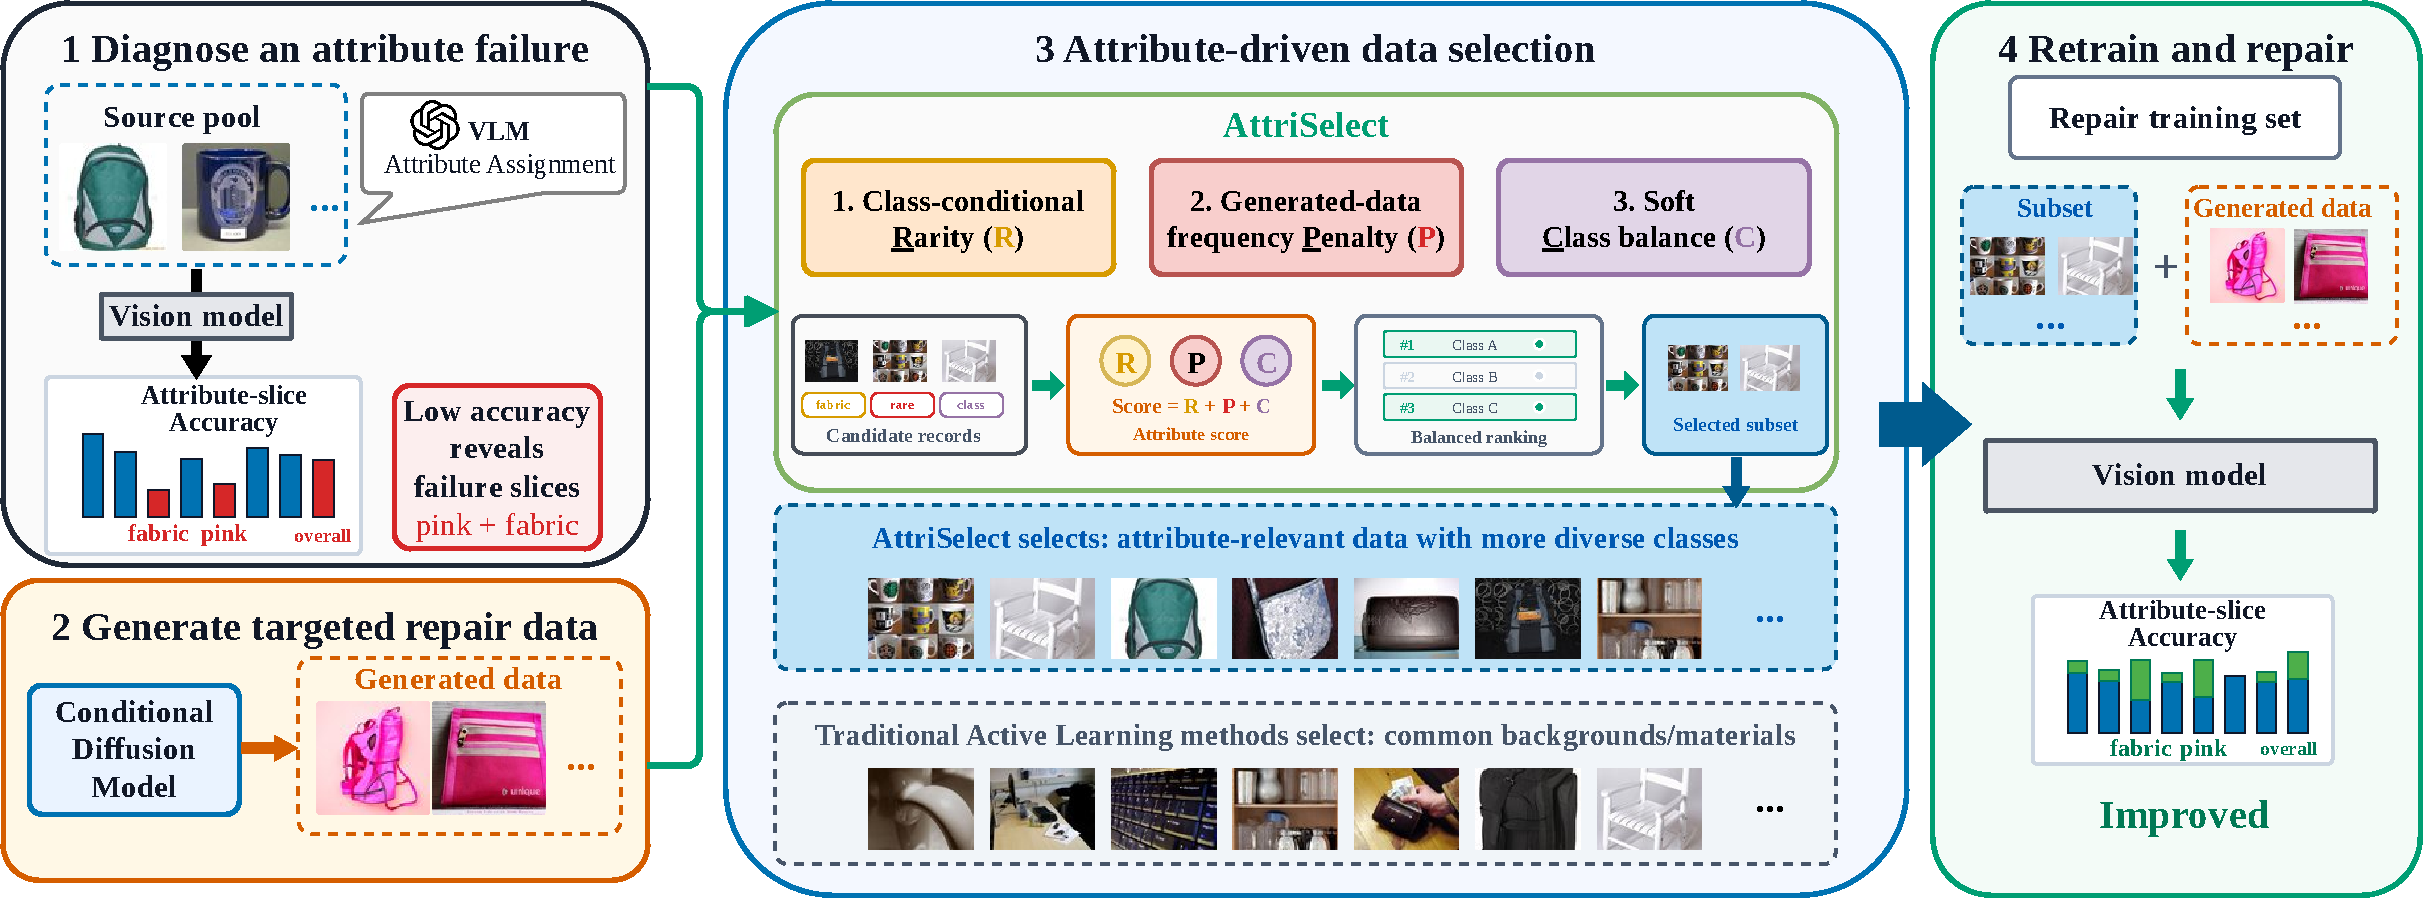
\includegraphics[width=\linewidth]{figures/show/11attriselect_framework.pdf}
\caption{\model framework. Given a diagnosed failure slice and generated images, \model scores source examples with group-conditional rarity, generated-data frequency penalty, and soft group balance, then returns an attribute-driven subset for retraining with the generated repair set.}
\label{fig:attriselect-framework}
\end{figure*}

\model is designed as the selection step inside an existing targeted repair pipeline. Figure~\ref{fig:attriselect-framework} summarizes this workflow. The upstream workflow can follow the model-repair systems described above. We distinguish the full task-level vocabulary $\attrs$ from the selector fields $\selattrs$ passed to the attribute-selection procedure. The target fields $\targetattrs$ define the diagnosed conjunction and generated repair pool; $\selattrs$ may include additional contextual fields retained for source selection. Qwen3-VL~\citep{bai2025qwen3vl} assigns an attribute value $v_{i,a}$ to each training or validation image. Appendix~\ref{app:attribute-assignment-details} gives the task-specific vocabularies and assignment protocol. Appendix~\ref{app:vlm-human-audit} reports a human audit and attribute-noise sensitivity, while Appendix~\ref{app:additional-robustness} evaluates incomplete target-field coverage. Using the SafeFix-style ImageNet10 classification setting as a running example, a ResNet-18 classifier is then trained to a checkpoint $\theta_t$, after which the repair pipeline analyzes the validation behavior of $f_{\theta_t}$. An attribute slice $T_{\mathrm{bug}}$ is marked as a rare failure case if it is underrepresented in training and underperforms on validation:
\begin{equation}
\label{eq:rare-failure-slice}
|T_{\mathrm{bug}}\cap\dataset_{\mathrm{train}}| < \rho |\dataset_{\mathrm{train}}|,
\qquad
\mathrm{Acc}(T_{\mathrm{bug}}) < \mathrm{Acc}(\dataset_{\mathrm{val}}),
\end{equation}
where $\rho$ is a user-specified rarity threshold. For example, the ImageNet10 pipeline may diagnose a slice whose attribute is \emph{texture} and whose value is \emph{fabric}. A conditional diffusion model, such as ControlNet~\citep{zhang2023adding}, then generates repair images of objects with fabric texture while preserving the class label and other attributes.

\model starts after this upstream diagnosis and generation stage. It takes as input the diagnosed slice, the original source pool with VLM-assigned attributes, and the generated repair images for that slice. The output is a compact source subset $\dataset_{\mathrm{sel}}^{\mathrm{src}}$, which is combined with the generated images and used to continue training or fine-tune the checkpoint $\theta_t$. \model does not replace VLM-based attribute proposal, failure-slice discovery, or conditional image generation. It decides which original training examples should accompany the generated repair data so that retraining preserves source coverage while allocating more budget to real examples that complement the diagnosed repair slice. Appendix~\ref{app:source-only-selection} separately evaluates the selection rule without a repair checkpoint, diagnosed slice, or generated data, including one-shot and iterative active-learning settings with multiple attribute sources.

\subsection{Attribute-Driven Active Learning}

Given $\dataset_{\mathrm{src}}$ and $\dataset_{\mathrm{gen}}$ for a discovered slice, the goal is to choose a small source subset that still supports the repair. Active learning is a natural tool for this problem: entropy-based uncertainty sampling selects examples with high predictive entropy, while CoreSet, BADGE, PPAL, and Uncertainty Herding add coverage, gradient diversity, or detector-side difficulty signals.

For targeted repair, however, the subset must answer a semantic question: which real images best complement the generated examples for the diagnosed failure slice? A subset may provide good coverage of the source distribution in terms of class labels or feature space while still containing very few examples from the rare failure slice itself. Likewise, entropy-based sampling can miss the slice entirely if the model assigns higher uncertainty to unrelated images. Selection signals must correlate with slice membership to increase its representation above the group base rate.

A second challenge arises because generated repair images alter the attribute distribution seen during retraining. If the generated pool already contains many examples with a target attribute, the source selector should not continue allocating most of its remaining budget to redundant examples of the same attribute. For instance, if generated repair images already emphasize rainy weather, a purely attribute-greedy selector may over-select common rainy street scenes while failing to retain rainy examples from underrepresented classes, unusual viewpoints, or occluded settings. This can bias the repair process toward the easiest contexts in which the target attribute appears.

\model uses a three-part scoring function to avoid these failure modes. First, the \textbf{group-conditional rarity} term scores marginal attribute values that are rare within their selection group. Second, the \textbf{generated-data frequency penalty} downweights attribute values that are already well represented by the generated repair images, reducing redundancy between synthetic and source data. Third, the \textbf{soft group-balance} term encourages coverage across selection groups by increasing the priority of groups that have received insufficient source budget. The combined score is intended to favor source examples carrying repair-relevant values without collapsing onto repeated synthetic attributes or a small number of easy groups. Because the score sums marginal field terms, it does not in general guarantee that a conjunction-defined slice receives the highest score; the conditional guarantee is stated in Proposition~\ref{prop:rarity-margin}.

\noindent\textbf{Group-conditional marginal rarity.} For a source image $x_i$, let $g_i$ denote its selection group and let $v_{i,a}$ be the value of attribute $a$ on that image. For ImageNet10 and CelebA, $g_i$ is the benchmark class label. For dense prediction tasks, the task-specific construction of $g_i$ is given in Appendix~\ref{app:implementation-details}. The rarity term gives higher weight to marginal attribute values that occur fewer times within the same selection group:
\begin{equation}
\label{eq:rarity-term}
\textcolor{colorR}{R_{i,a}} = \left(\frac{1}{n_a(v_{i,a}\mid g_i)+\varepsilon}\right)^{\alpha}
\end{equation}
where $n_a(v_{i,a}\mid g_i)$ is the number of source examples in selection group $g_i$ whose attribute $a$ takes value $v_{i,a}$, $\varepsilon > 0$ is a numerical stability constant, and $\alpha \geq 0$ controls how strongly the selector prefers rare attribute values.

This term remains important even after adding generated repair images. Although generated images can make a target attribute less rare in the combined repair pool, they do not make real source examples with that attribute redundant, since the two data sources may differ in image statistics, contextual diversity, learned representations, and other unannotated visual factors. When a defining marginal value is rare within a selection group, group-conditional rarity helps retain real source examples carrying that value in the candidate ranking. It does not by itself measure the frequency of a multi-attribute conjunction. The role of the generated-data frequency penalty is complementary: rather than promoting rarity, it prevents this preference from repeatedly selecting attribute values that are already heavily represented in the generated repair data.

\noindent\textbf{Generated-data frequency penalty.} Rarity alone can over-select attribute values that are already well covered by the generated repair pool. In the rainy-weather example above, if the generated data already contains many rainy images, the selector should not spend most of its remaining source budget on additional easy rainy cases from similar contexts. Instead, it should retain useful real-source rainy examples while still leaving room for complementary classes, viewpoints, and occlusion patterns. To capture this trade-off, we measure how common each attribute value becomes after combining source and generated data as $\hat{n}_a(v) = n_a^{\mathrm{src}}(v) + \tilde{n}_a^{\mathrm{gen}}(v)$, where $n_a^{\mathrm{src}}(v)$ denotes the source count and $\tilde{n}_a^{\mathrm{gen}}(v)=\gamma_r n_a^{\mathrm{gen}}(v)$, with $\gamma_r$ denoting the task- and ratio-specific count scale. The main ImageNet10 and KITTI repair runs use $\gamma_r=1$, while the CelebA and COCO repair runs use $\gamma_r=1/r$. Attribute values with larger effective counts receive lower scores:
\begin{equation}
\label{eq:frequency-penalty}
\textcolor{colorP}{P_{i,a}} = -\lambda \cdot \frac{\hat{n}_a(v_{i,a})}{\sum\nolimits_{v \in \vals_a} \hat{n}_a(v)}
\end{equation}
where $\lambda \geq 0$ controls how strongly the selector penalizes already over-represented attribute values.

We then define the \textbf{base source score} $\bar{s}_i$ by summing the rarity and generated-data frequency terms over the selector fields:
\begin{equation} \label{eq:base-attribute-score} \bar{s}_i = \sum_{a \in \selattrs} \Big( \textcolor{colorR}{R_{i,a}} + \textcolor{colorP}{P_{i,a}} \Big). \end{equation}
Each component addresses a different failure mode in repair-time selection. Setting $\alpha=0$ removes the preference for rare marginal attribute values within a selection group, reducing the selector to a frequency-driven policy. Setting $\lambda=0$ removes the redundancy penalty, allowing the selected subset to repeatedly choose attribute values already well represented in $\dataset_{\mathrm{gen}}$. Without group-aware re-ranking, high-scoring examples may further concentrate within a small subset of groups. The score targets repair-specific semantic coverage rather than a neutral representative subset. Appendix~\ref{app:additional-repair-controls} compares the full score with a Generated-Complement control and reports the resulting class--attribute coverage, attribute diversity, and group balance of the selected subsets.

\noindent\textbf{Soft group balance.} Attribute scores are computed per image, so they can still over-select groups that happen to contain many high-scoring attributes. For example, in a fabric-texture repair, many high-scoring images may come from classes where fabric is visually common, while guitar images may contain the texture only in straps or carrying cases. We correct this with a soft group-balance term. Let $n_{\text{select}}$ be the source-data budget and let $N_{\mathrm{grp}}$ be the number of active selection groups, so the per-group target is $t = n_{\text{select}} / N_{\mathrm{grp}}$. During greedy selection step $k$, a candidate from group $g$ receives the adjusted score
\begin{equation}
\label{eq:class-balance-score}
\tilde{s}_i^{(k)} = \bar{s}_i + \textcolor{colorC}{C_g^{(k)}}, \qquad
\textcolor{colorC}{C_g^{(k)}} = w \cdot \frac{t - n_g^{(k)}}{t},
\end{equation}
where $n_g^{(k)}$ is the number of already selected source samples from group $g$, and $w \geq 0$ controls the strength of soft group balancing. Groups below their target allocation receive a positive correction, while groups above their target receive a negative one. As $w$ increases, the selector behaves more like stratified sampling, with the limiting case $w=\infty$ corresponding to round-robin group quotas. This mechanism preserves the attribute-based ranking from Eq.~\ref{eq:base-attribute-score} within each group while preventing a small subset of groups from dominating the repair set.

Selection is performed greedily. We first compute the base score $\bar{s}_i$ for every source candidate and initialize both the selected set and the per-group counts to zero. At each iteration, every remaining candidate receives the adjusted score $\tilde{s}_i^{(k)}$ from Eq.~\ref{eq:class-balance-score}. The highest-scoring candidate is then added to $\dataset_{\mathrm{sel}}^{\mathrm{src}}$, its group count is updated, and the soft group-balance corrections are recomputed. The process repeats until $n_{\text{select}}$ source examples have been selected. The generated repair set remains fixed throughout this procedure and influences selection only through the effective frequency counts in Eq.~\ref{eq:frequency-penalty}. All methods use the same fixed generated-data budget. Appendix~\ref{app:attriselect-algorithm} gives the full pseudocode, and Appendix~\ref{app:hyperparameter-details} reports the score hyperparameters used in the experiments.

\subsection{Theoretical Analysis}
\label{subsec:slice-enrichment}

Useful repair subsets should contain examples from the diagnosed failure slice while preserving source coverage. The following analysis gives conditions under which the marginal attribute score enriches that slice. Let $T\subseteq\dataset_{\mathrm{src}}$ denote the target failure slice. Here $c$ denotes a selection group: the benchmark class for classification or the task-specific proxy group for dense prediction (Appendix~\ref{app:implementation-details}). Write $T_c=T\cap\{x_i:g_i=c\}$ and $N_c=|\{x_i:g_i=c\}|$.

\begin{tcolorbox}[
    colback=blue!2!white,
    colframe=blue!20!white,
    arc=3pt,
    boxrule=1pt,
    before skip=3pt,
    after skip=3pt,
    top=3pt,
    bottom=3pt,
    boxsep=1pt,
    drop shadow,
    breakable
]
\begin{proposition}[Conditional target-slice enrichment]
\label{prop:rarity-margin}
For $x_i\in T_c$ and $x_j\notin T_c$ in the same group, define $A_{ij}=\sum_{a\in\selattrs}(R_{i,a}-R_{j,a})$ and
\begin{equation*}
F_{ij}=\sum_{a\in\selattrs}
\frac{\hat n_a(v_{i,a})-\hat n_a(v_{j,a})}{\sum_{v\in\vals_a}\hat n_a(v)}.
\end{equation*}
Suppose $A_{ij}>0$ for every such pair and $0\leq\lambda<\lambda_c^\star$, where $\lambda_c^\star=\min_{i\in T_c,\,j\notin T_c,\,F_{ij}>0}A_{ij}/F_{ij}$ and the minimum of an empty set is $\infty$. If the selector draws $B_c$ source examples from group $c$, then
\begin{equation}
\label{eq:deterministic-enrichment-bound}
|\dataset_{\mathrm{sel}}^{\mathrm{src}}\cap T_c|=\min\{B_c,|T_c|\}.
\end{equation}
Uniform sampling of $B_c$ examples from the same group instead gives $\mathbb{E}[|S_{\mathrm{rand}}\cap T_c|]=B_c|T_c|/N_c$.
\end{proposition}
\end{tcolorbox}

The result depends on every target example outranking every non-target example within the group and on the realized allocation $B_c$; it does not guarantee a positive allocation or improved trained-model performance. The score sums marginal terms, so a rare conjunction whose marginal values are common may fail the condition. The comparison with uniform sampling holds for the same $B_c$ and uniform sampling within group $c$. Other AL methods can enrich the slice when their selection signals align with it.

Geometric coverage alone also gives no fixed bound on how many target examples a global CoreSet solution selects. Appendix~\ref{app:theory-analysis} separates this local covering observation from the ranking guarantee and gives a stepwise bound for the finite soft-balance weight $w$.

\noindent The proof and the count conditions are in Appendix~\ref{app:theory-analysis}.

\section{Experiments}

\paragraph{Datasets and Tasks}
We evaluate \model on three vision tasks: image classification, pose estimation, and object detection. In all settings, the goal is to test whether attribute-aware source-data selection can choose a subset that improves the model performance and fixes bugs.

For image classification, we follow \safefix~\citep{xu2025safefix}: a ResNet-18 classifier on an ImageNet subset~\citep{deng2009imagenet} with 10 classes, 1,300 images per class, and an 8:1:1 train/validation/test split, denoted ImageNet10. We also evaluate CelebA~\citep{liu2015deep} lipstick-wearing classification with a ResNet-18-based binary classifier and 80,000/10,000/10,000 train/validation/test images. For pose estimation, we follow HiBug2~\citep{chen2025hibug2} on COCO person keypoints~\citep{lin2014microsoft}, using Keypoint R-CNN~\citep{mask-rcnn-2017} with a ResNet-50-FPN backbone~\citep{he2016deep}, 20,000 source training images, and 1,173-image held-out validation and test splits, evaluated by COCO keypoint AP. For object detection, we use KITTI~\citep{geiger2012we} Car and Pedestrian instances converted to YOLO format with 5,000/1,240/1,241 train/validation/test images, and train YOLOv8n. Implementation details are given in Appendix~\ref{app:implementation-details}.

\paragraph{Metrics}
Let $M$ denote the task metric: test accuracy for image classification, COCO keypoint AP for pose estimation, and mAP50--95 for object detection. We focus on targeted improvements for failure cases, which are critical for fairness and safety, while also tracking overall task performance. We report Relative Error Reduction (RER),
\begin{equation}
\mathrm{RER}(\%)=100\cdot\frac{M_{\mathrm{after}}-M_{\mathrm{before}}}{1-M_{\mathrm{before}}},
\end{equation}
where $M_{\mathrm{before}}$ and $M_{\mathrm{after}}$ are the test metrics before and after repair. In the main RER tables, $M_{\mathrm{before}}$ is $933/1300\approx0.7177$ for ImageNet10, $0.9057$ for CelebA, $0.5902$ for COCO, and $0.5626$ for KITTI. For accuracy, RER is the percentage of the original error rate removed by repair; for AP and mAP, it is the normalized improvement toward the maximum score, reported in percent.

\paragraph{Baselines}
We compare \model with seven source-selection baselines. \textbf{\textsc{Random}} samples images uniformly at random. \textbf{\textsc{Stratified}} preserves class proportions during sampling~\citep{neyman1934two}. \textbf{\textsc{Entropy}} selects examples with the largest predictive entropy or task-specific confidence-entropy proxy. \textbf{\textsc{CoreSet}} uses greedy coverage in embedding space. \textbf{\textsc{BADGE}} selects gradient-embedding batches that combine uncertainty and diversity~\citep{settles2009active,sener2018active,ash2020deep}. \textbf{\textsc{PPAL}} is a plug-and-play active-learning baseline for object detection. \textbf{\textsc{UHerding}} denotes Uncertainty Herding, which combines uncertainty with coverage across label budgets~\citep{yang2024ppal,bae2025uncertainty}.

The seven generic baselines do not receive the repair attributes used by \model. Appendix~\ref{app:additional-repair-controls} therefore adds matched-information baselines that use the same target fields through direct filtering, stratification, entropy ranking, or generated-set complementarity.

\subsection{Main Results}

Table~\ref{tab:main-rer} compares \model with generic source-selection baselines using RER. All main-result entries are averaged over five random seeds. The original task metrics and variance over five seeds are reported in Appendix~\ref{app:main-metric-tables}.

\noindent\textbf{Analysis.} \model gives the best RER in almost all active source-selection settings, excluding the ratio-$1.0$ full-data references where all selectors are identical. The gap is largest at small budgets, where the selected source subset is highly constrained, and it generally remains at larger budgets. KITTI is the only near-exception: PPAL is slightly higher at ratio $0.7$ by $0.05$ RER points, while \model remains best at the other four KITTI ratios. Appendix~\ref{app:image-generation-effect} reports the same selector ordering under an alternative repair pipeline and alternative generators, and Appendix~\ref{app:additional-robustness} shows that the ImageNet10 ordering persists across longer repair schedules.

Subset selection can also outperform the full-data setting, especially on ImageNet10, CelebA, and COCO. Appendix~\ref{app:additional-repair-controls} reports that \model remains strongest at the more constrained source ratios $0.02$ and $0.05$ and quantifies the class--attribute coverage and diversity of the selected subsets. The t-SNE visualizations in Appendix~\ref{app:selection-tsne} compare its selected regions with those of generic AL baselines across varied visual contexts.

KITTI behaves differently at the smallest source budget. At ratio $0.1$, all methods have negative RER. A likely reason is that KITTI has only $5{,}000$ training images, so the selected source subset contains just $500$ real images, unlike ImageNet10, COCO, and CelebA where the same ratio still leaves thousands to tens of thousands of source examples. This is a low-data failure mode: for small detection datasets, an overly small repair subset may not retain enough background, viewpoint, and object-scale variation to improve over the original detector. Under the same generated repair set and source budget, \model remains the least damaging option and has the highest RER in this row.

\begin{table*}[t]
\centering
\caption{Main repair results across tasks, averaged over five random seeds. Metric: RER (\%).}
\label{tab:main-rer}
\small
\setlength{\tabcolsep}{3pt}
\renewcommand{\arraystretch}{0.98}
\begin{tabular}{l c c c c c c c c >{\columncolor{myblue!8}}c}
\toprule
\rowcolor{sectiongray} \firstrowstrut\textbf{Dataset} & Ratio & Random & Stratified & Entropy & CoreSet & BADGE & UHerding & PPAL & \cellcolor{myblue!8}\textbf{Ours} \\
\midrule
\multirow{6}{*}{ImageNet10}
& 0.1 & 3.27 & 3.32 & 2.72 & 3.27 & 5.18 & 5.45 & 3.81 & \textbf{6.81} \\
& 0.3 & 4.63 & 6.81 & 4.09 & 6.81 & 8.72 & 10.35 & 7.63 & \textbf{11.17} \\
& 0.5 & 7.19 & 9.54 & 5.45 & 7.90 & 10.35 & 8.23 & 8.72 & \textbf{11.72} \\
& 0.7 & 8.72 & 5.99 & 6.27 & 7.63 & 10.63 & 10.35 & 8.72 & \textbf{11.99} \\
& 0.9 & 10.08 & 10.35 & 10.08 & 5.99 & 9.26 & 11.44 & 11.72 & \textbf{13.62} \\
\noalign{\vskip 1.5pt}\cdashline{3-10}\noalign{\vskip 1.5pt}
& 1.0 & 7.90 & 7.90 & 7.90 & 7.90 & 7.90 & 7.90 & 7.90 & 7.90 \\
\midrule
\multirow{6}{*}{CelebA}
& 0.1 & 4.88 & 2.44 & 7.10 & -6.04 & 3.18 & -1.06 & 5.94 & \textbf{8.48} \\
& 0.3 & 6.04 & 5.30 & 8.70 & 7.95 & 1.91 & 3.50 & 4.03 & \textbf{10.50} \\
& 0.5 & 6.04 & 7.95 & 7.64 & 8.17 & 2.86 & 2.23 & 9.97 & \textbf{13.79} \\
& 0.7 & 2.86 & 8.27 & 10.18 & 6.57 & 8.06 & 5.09 & 6.04 & \textbf{12.09} \\
& 0.9 & 3.18 & 4.56 & 8.27 & 6.04 & 6.04 & 4.56 & 6.57 & \textbf{14.74} \\
\noalign{\vskip 1.5pt}\cdashline{3-10}\noalign{\vskip 1.5pt}
& 1.0 & 6.04 & 6.04 & 6.04 & 6.04 & 6.04 & 6.04 & 6.04 & 6.04 \\
\midrule
\multirow{6}{*}{COCO}
& 0.1 & 3.56 & 5.08 & 5.61 & -0.61 & 2.03 & 2.71 & 1.17 & \textbf{6.86} \\
& 0.3 & 3.37 & 8.32 & 7.64 & 8.64 & 6.12 & 4.32 & 6.42 & \textbf{9.86} \\
& 0.5 & 7.49 & 8.00 & 9.27 & 6.47 & 7.42 & 6.12 & 6.83 & \textbf{10.13} \\
& 0.7 & 6.08 & 9.69 & 9.54 & 9.10 & 8.64 & 6.17 & 7.83 & \textbf{10.18} \\
& 0.9 & 4.61 & 9.49 & 6.54 & 7.32 & 7.59 & 7.05 & 9.74 & \textbf{11.05} \\
\noalign{\vskip 1.5pt}\cdashline{3-10}\noalign{\vskip 1.5pt}
& 1.0 & 8.71 & 8.71 & 8.71 & 8.71 & 8.71 & 8.71 & 8.71 & 8.71 \\
\midrule
\multirow{6}{*}{KITTI}
& 0.1 & -9.65 & -7.27 & -7.52 & -8.89 & -6.95 & -9.24 & -8.32 & \textbf{-5.81} \\
& 0.3 & -0.48 & -1.23 & 0.23 & -0.32 & -0.05 & -1.21 & -1.33 & \textbf{0.46} \\
& 0.5 & 2.13 & 1.23 & 3.20 & 3.04 & 2.29 & 1.12 & 2.17 & \textbf{3.36} \\
& 0.7 & 3.20 & 3.06 & 3.34 & 3.34 & 2.08 & 3.25 & \textbf{3.57} & 3.52 \\
& 0.9 & 4.37 & 4.66 & 4.66 & 3.54 & 4.21 & 4.85 & 3.89 & \textbf{5.12} \\
\noalign{\vskip 1.5pt}\cdashline{3-10}\noalign{\vskip 1.5pt}
& 1.0 & 5.30 & 5.30 & 5.30 & 5.30 & 5.30 & 5.30 & 5.30 & 5.30 \\
\bottomrule
\end{tabular}
\end{table*}

\subsection{Computational Efficiency}

After attribute records are available, \model is also cheaper than generic active-learning selectors. Its
selection cost is dominated by counting VLM-assigned attribute values and
sorting candidates, while uncertainty, coverage, and gradient-embedding
baselines require model scoring, embedding comparisons, or iterative diversity
updates. Table~\ref{tab:selection-efficiency} reports source-subset selection
time on COCO and CelebA for the three ratios used in the main small-to-medium
budget comparison. The source pools contain 20,000 COCO training images and
80,000 CelebA training images. Random and stratified sampling have negligible
algorithmic selection cost after excluding data loading and export overhead;
we keep them in the table as zero-cost references.

\begin{table*}[t]
\centering
\caption{Source-subset selection time. Units are seconds (s), minutes (m), and hours (h). Speedup is measured against the fastest non-attribute active-learning baseline in the same row.}
\label{tab:selection-efficiency}
\small
\setlength{\tabcolsep}{3pt}
\renewcommand{\arraystretch}{1.0}
\begin{tabular}{l c c c c c c c c >{\columncolor{myblue!8}}c}
\toprule
\rowcolor{sectiongray} \firstrowstrut Dataset & Ratio & Random & Stratified & Entropy & CoreSet & BADGE & UHerding & PPAL & \cellcolor{myblue!8}\textbf{Ours / speedup} \\
\midrule
COCO & 0.1 & 0s & 0s & 563s & 5m & 21m & 86s & 67s & \textbf{0.29s / 231$\times$} \\
COCO & 0.3 & 0s & 0s & 565s & 15m & 1h & 93s & 85s & \textbf{0.30s / 283$\times$} \\
COCO & 0.5 & 0s & 0s & 566s & 25m & 2h & 94s & 90s & \textbf{0.32s / 281$\times$} \\
\midrule
CelebA & 0.1 & 0s & 0s & 49s & 45m & 2h & 63s & 46s & \textbf{0.42s / 110$\times$} \\
CelebA & 0.3 & 0s & 0s & 51s & 3h & 5h & 65s & 51s & \textbf{0.51s / 100$\times$} \\
CelebA & 0.5 & 0s & 0s & 54s & 5h & 9h & 61s & 61s & \textbf{1.37s / 39$\times$} \\
\bottomrule
\end{tabular}
\end{table*}

\model selects each subset in less than two seconds. The fastest non-attribute
active-learning baseline takes tens of seconds, and coverage or
gradient-embedding methods can take minutes to hours. Even against the fastest
nontrivial baseline in each row, \model is at least $39\times$ faster on
CelebA and more than $230\times$ faster on COCO. These are source-subset selection speedups, not end-to-end pipeline speedups. Appendix~\ref{app:end-to-end-cost} reports end-to-end wall-clock time.

\subsection{Attribute-Slice Accuracy Differences}

For each attribute slice, we report the accuracy difference
$M_{\mathrm{after}}-M_{\mathrm{before}}$, where $M_{\mathrm{before}}$ is
measured at the original vision model checkpoint $\theta_t$ and
$M_{\mathrm{after}}$ is measured after retraining. For ImageNet10
classification, $M$ is accuracy. Positive values therefore indicate
slice-level improvement after repair. Figure~\ref{fig:imagenet-ratio05-attribute-delta} reports these differences for ImageNet10 at source ratio $0.5$.

\begin{figure}[t]
\centering
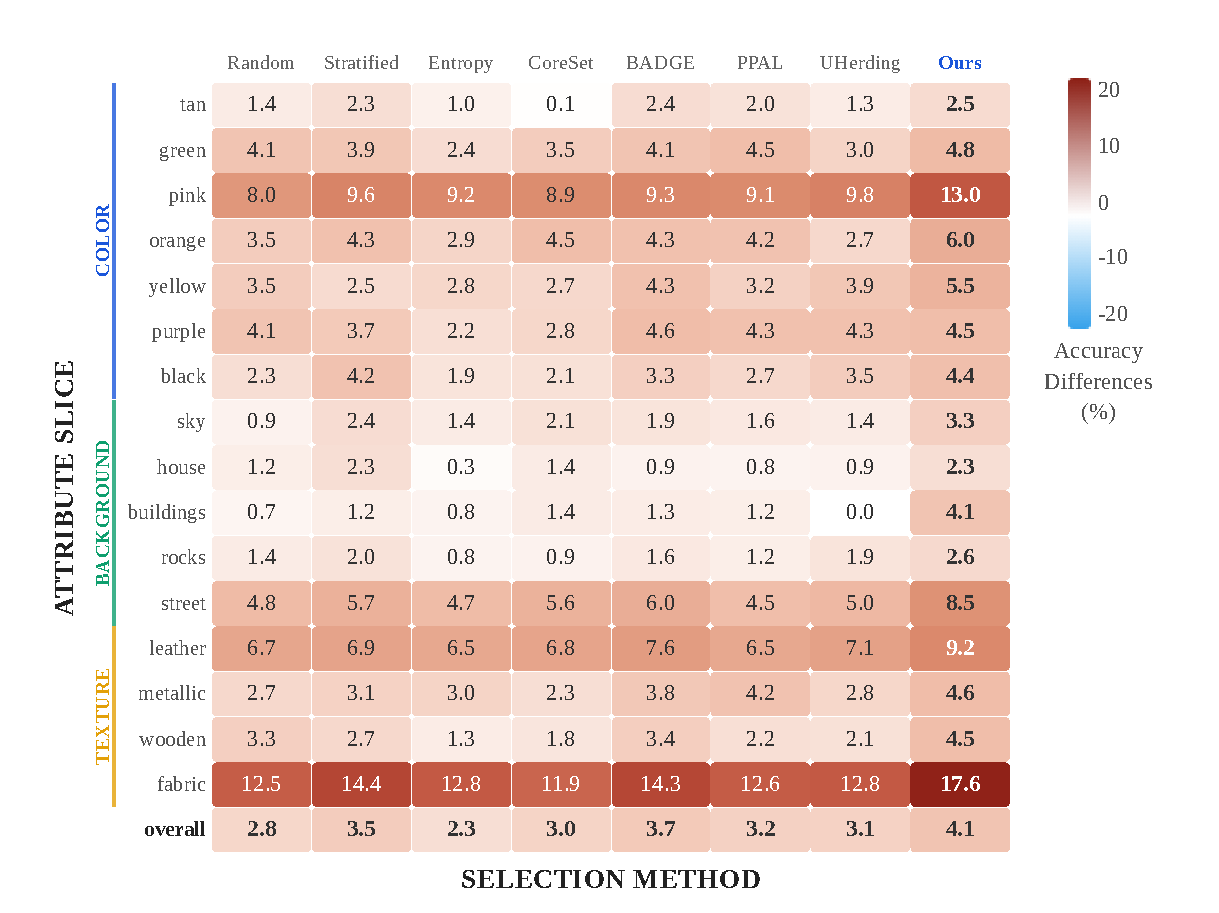
\includegraphics[width=\linewidth,trim={0 12pt 0 28pt},clip]{figures/show/heatmap_.pdf}
\caption{ImageNet10 ratio-$0.5$ attribute-slice accuracy differences. \model gives larger gains on the targeted attribute families, with the strongest gains on the exact repair values.}
\label{fig:imagenet-ratio05-attribute-delta}
\end{figure}

All methods use the same generated repair images and differ only in the
selected source subset. The generated data targets pink color and fabric
texture. \model gives the largest gains on the targeted attribute families,
especially the exact repair values pink and fabric. The selected source subset
improves target-slice alignment rather than only changing overall accuracy.
Appendix~\ref{app:attribute-slice-heatmaps} provides
the COCO pose-estimation heatmap over the full annotated vocabulary.
Because these heatmaps show marginal attribute values, Appendix~\ref{app:additional-repair-controls}
also reports the full diagnosed conjunction and its strict complement.
Appendix~\ref{app:additional-robustness} evaluates how the result changes when
the slice uses one, two, or three target fields.

\subsection{Failure-Slice Repair Counts}

\begin{table}[t]
\centering
\caption{COCO repaired slices out of 12.}
\label{tab:coco-bug-repair-counts}
\small
\setlength{\tabcolsep}{3pt}
\renewcommand{\arraystretch}{0.9}
\begin{tabular}{c c >{\columncolor{myblue!8}}c}
\toprule
\firstrowstrut Ratio & Best AL & Ours \\
\midrule
0.1 & 7 & \textbf{10} \\
0.3 & 8 & \textbf{10} \\
0.5 & 10 & \textbf{11} \\
0.7 & 10 & \textbf{11} \\
0.9 & 10 & \textbf{11} \\
\bottomrule
\end{tabular}
\end{table}

We also evaluate repair at the level of discovered failure slices. In the
upstream bug-discovery stage for COCO, 12 failure slices are identified. With
the proposed framework, \model repairs 10 of these slices already at source
ratio $0.1$, whereas the strongest active-learning baseline repairs 7 slices
at the same ratio. The strongest baseline reaches 10 repaired slices only from
source ratio $0.5$ onward, while \model repairs 11 slices at ratios $0.5$,
$0.7$, and $0.9$.

\subsection{Ablation Study}

We ablate the three score components on ImageNet10 classification repair to test whether the gains come from a single term or from their combination. Table~\ref{tab:imagenet-rpc-ablation} reports test accuracy for all component subsets. The full $\textcolor{colorR}{R}+\textcolor{colorP}{P}+\textcolor{colorC}{C}$ setting combines rarity $\textcolor{colorR}{R}$, generated-data frequency penalty $\textcolor{colorP}{P}$, and soft class balance $\textcolor{colorC}{C}$; it gives the best result at every ratio. The leave-one-component-out drops are nearly identical: removing $\textcolor{colorR}{R}$ drops test accuracy by $0.00945$ on average, removing $\textcolor{colorP}{P}$ by $0.00938$, and removing $\textcolor{colorC}{C}$ by $0.00938$. These results support complementarity rather than a single dominant component on ImageNet10. Single-component variants are also weaker on average ($\textcolor{colorR}{R}$: $0.74200$, $\textcolor{colorP}{P}$: $0.74037$, $\textcolor{colorC}{C}$: $0.73815$) than the full setting ($0.74892$). A COCO pose-estimation component ablation with a broadly similar trend is reported in Appendix~\ref{app:coco-rpc-ablation}.

\begin{table*}[t]
\centering
\caption{ImageNet10 classification attribute-score component ablation. Metric: test accuracy.}
\label{tab:imagenet-rpc-ablation}
\small
\setlength{\tabcolsep}{4pt}
\renewcommand{\arraystretch}{0.95}
\begin{tabular}{c c c c c c c c >{\columncolor{myblue!8}}c}
\toprule
\firstrowstrut Ratio & none & $\textcolor{colorR}{R}$ & $\textcolor{colorP}{P}$ & $\textcolor{colorC}{C}$ & $\textcolor{colorP}{P}+\textcolor{colorC}{C}$ & $\textcolor{colorR}{R}+\textcolor{colorC}{C}$ & $\textcolor{colorR}{R}+\textcolor{colorP}{P}$ & \cellcolor{myblue!8}$\textcolor{colorR}{\boldsymbol{R}}+\textcolor{colorP}{\boldsymbol{P}}+\textcolor{colorC}{\boldsymbol{C}}$ \\
\midrule
0.1 & 0.7269 & 0.7300 & 0.7262 & 0.7277 & 0.7358 & 0.7308 & 0.7315 & \textbf{0.7369} \\
0.3 & 0.7308 & 0.7415 & 0.7392 & 0.7392 & 0.7308 & 0.7369 & 0.7315 & \textbf{0.7492} \\
0.5 & 0.7400 & 0.7415 & 0.7408 & 0.7346 & 0.7369 & 0.7415 & 0.7446 & \textbf{0.7508} \\
0.7 & 0.7423 & 0.7469 & 0.7431 & 0.7415 & 0.7431 & 0.7469 & 0.7477 & \textbf{0.7515} \\
0.9 & 0.7462 & 0.7500 & 0.7526 & 0.7477 & 0.7508 & 0.7415 & 0.7423 & \textbf{0.7562} \\
\bottomrule
\end{tabular}
\end{table*}
% We conduct experiments on ImageNet-10 (multi-class) and CelebA (binary, targeting the `redhair\_brownskin' subgroup correlation). We employ a standard ResNet-18 architecture, initiating with pretrained weights and utilizing the AdamW optimizer. 

% \subsection{\model vs. Long-Tail Learning Baselines}

% We isolate the effect of \model against four standard LTL algorithms: Focal Loss \citep{lin2017focal}, Class-Balanced Loss, Oversampling (via WeightedRandomSampler), and LDAM Loss \citep{cao2019learning}. To ensure a fair comparison, the LTL baselines were trained exclusively on the original datasets without access to the targeted synthetic augmentation provided by \model.

% \begin{table*}[t]
% \caption{Performance comparison of \model vs. LTL baselines on ResNet-18. \model leverages synthetic subgroups, effectively rescuing bugs where standard reweighting methods fail.}
% \centering
% \begin{tabular}{l cc cc}
% \toprule
% \textbf{Method} & \textbf{CelebA Test ACC} & \textbf{Fix Bugs} & \textbf{ImageNet Test ACC} & \textbf{Fix Bugs} \\
% \midrule
% Base Model & 90.57\% & - & 71.73\% & - \\
% Focal Loss & 91.40\% & 8/13 & 68.80\% & 11/17 \\
% Class-Balanced Loss & 91.20\% & 8/13 & 72.70\% & 13/17 \\
% Oversampling & 91.00\% & 8/13 & 72.90\% & 14/17 \\
% LDAM & 91.40\% & 8/13 & 71.20\% & 12/17 \\
% \midrule
% \textbf{/model (Ours)} & \textbf{91.92\%} & - & \textbf{74.88\%} & - \\
% \bottomrule
% \end{tabular}
% \end{table*}

% The results demonstrate that while algorithmic reweighting techniques provide marginal improvements over the base model, they are fundamentally insufficient for repairing unannotated, intersectional attribute failures compared to SafeFix's target-augmented methodology.

% \subsection{Active Learning Strategy Ablations}

% To validate the efficiency of our Attribute-Driven strategy in curating augmented datasets, we compare it against standard Active Learning regimes across various integration sub-ratios ($0.1$ through $0.9$). The models were trained learning rate of $1e-5$ for 15 epochs. 

% \begin{table*}[t]
% \caption{Comparison of Top-Performing Selection Strategies on ImageNet (ResNet-18) at various subset sampling ratios. Our Attribute strategy utilizes generated captions from LLMs (BLIP, Qwen3, InternVL3).}
% \centering
% \resizebox{\columnwidth}{!}{
% \begin{tabular}{l ccc c}
% \toprule
% \textbf{Strategy} & \textbf{Ratio=0.1} Test/Val & \textbf{Ratio=0.3} Test/Val & \textbf{Ratio=0.5} Test/Val & \textbf{Ratio=0.9} Test/Val \\
% \midrule
% Random & 0.7269 / 0.7069 & 0.7308 / 0.7208 & 0.7400 / 0.7162 & 0.7482 / 0.7154 \\
% Stratified & 0.7271 / 0.7154 & 0.7369 / 0.7162 & 0.7446 / 0.7200 & 0.7469 / 0.7146 \\
% Coreset & 0.7269 / 0.7115 & 0.7369 / 0.7162 & 0.7400 / 0.7185 & 0.7346 / 0.7169 \\
% Uncertainty Stratified & 0.7254 / 0.7185 & 0.7292 / 0.7131 & 0.7331 / 0.7146 & 0.7462 / 0.7100 \\
% Hierarchical & 0.7269 / 0.7115 & 0.7346 / 0.7092 & 0.7385 / 0.7138 & 0.7362 / 0.7177 \\
% \midrule
% Attribute (BLIP) & 0.7277 / 0.7200 & 0.7369 / 0.7185 & 0.7408 / 0.7131 & 0.7400 / 0.7177 \\
% Attribute (Qwen3) & 0.7331 / 0.7231 & 0.7354 / 0.7077 & 0.7362 / 0.7138 & 0.7492 / 0.7108 \\
% \textbf{Attribute (InternVL3)} & \textbf{0.7346} & \textbf{0.7385} & \textbf{0.7495} & \textbf{0.7531} \\
% \bottomrule
% \end{tabular}
% }
% \end{table*}

% The Attribute-Driven strategy continuously outperforms traditional geometry-based (Coreset) and balanced (Stratified) methodologies at almost every data budget. Further utilizing advanced Vision-Language Models like InternVL3 to source the attribute metadata yields compounding performance benefits.


% \subsection{Parameter Scaling Analysis}

% By adjusting the weights of $R$, $P$, and $C$, we explored the behavioral boundaries of our strategy (sub-ratio $0.3$). 

% \begin{itemize}
%     \item \textbf{Pure Greedy ($R=1.0, P=10.0, C=0.0$)}: Test ACC 0.7215. Without class-level Stratification quotas, throwing out all logic except Frequency Penalty and Rarity leads to performance drops in fine-tuning, emphasizing the value of our soft $C$ score.
%     \item \textbf{Aggressive Exploration ($R=0.8, P=10.0, C=4.0$)}: Test ACC \textbf{0.7415}. By loosening the absolute restriction on stratification and vastly scaling up Rarity tracking, the model dynamically locates critical edge cases. The extreme Frequency Penalty ($P=10$) adequately prevents the network from collapsing entirely onto the synthetic injection vectors.
% \end{itemize}

\section{Conclusion}

We studied targeted vision model repair as a repair-time source-selection problem. In this setting, a failure slice has been diagnosed and targeted repair images have been generated; the remaining question is which source examples should accompany those generated images during retraining. \model addresses this question with an attribute-driven score that combines class-conditional marginal rarity, generated-data frequency control, and soft class balancing. The analysis identifies conditions under which this score enriches a target slice relative to attribute-agnostic selectors; rarity of a conjunction alone does not imply this condition. Across classification, pose estimation, and detection, structured attribute metadata adds a repair-specific signal beyond uncertainty, coverage, and gradient embeddings. \model serves as one component in a localized repair pipeline rather than a replacement for upstream bug discovery or image generation.

\subsection*{AI use statement}

In this work, generative AI models, vision--language models (VLMs), and large language models (LLMs) were utilized in the upstream data and repair pipeline, for theoretical proof assistance, and for manuscript preparation:
\begin{itemize}[leftmargin=*,noitemsep,topsep=2pt]
    \item \textbf{Synthetic repair image generation:} Conditional diffusion models (\controlnet, InstructPix2Pix, and ICEdit) were employed to generate targeted synthetic repair images for diagnosed failure slices, as described in Section 3 and detailed in Appendix~\ref{app:image-generation-effect}.
    \item \textbf{Attribute annotation and image QA filtering:} LLMs (GPT-5) and VLMs (such as Qwen3-VL, BLIP, and InternVL3) were used in the upstream pipeline to propose candidate attribute taxonomies (Appendix~\ref{app:attribute-assignment-details}) and assign discrete attribute metadata to dataset images via visual question answering (VQA). In addition, VLMs served as semantic filters using image question answering to verify that generated synthetic images accurately exhibit the targeted failure attributes and preserve ground-truth task labels before retraining.
    \item \textbf{Theoretical proof assistance:} Large language models assisted with intermediate algebra, the presentation of derivations, and boundary-condition checks for some of the propositions in Appendix~\ref{app:theory-analysis}. The authors remain responsible for verifying the final mathematical statements and proofs.
    \item \textbf{Writing assistance:} LLMs were used solely for phrasing refinement, grammatical polishing, and formatting suggestions.
\end{itemize}
The reliability of VLM-assigned attributes was verified through an independent blinded human audit with five graduate students (Appendix~\ref{app:vlm-human-audit}). The authors have reviewed all AI-assisted outputs and take full responsibility for the final text, code, claims, and artifacts in this paper.

\subsection*{Ethics statement}

This research investigates targeted vision model repair to correct systematic failure slices and improve model reliability across diverse visual attributes. The empirical evaluation relies on standard, publicly available research benchmarks (ImageNet, CelebA, COCO, and KITTI). Synthetic data generation is strictly restricted to benign semantic attributes (such as color, texture, or clothing variations) for model debugging and fairness improvement, without generating sensitive, private, or defamatory content.

\subsection*{Reproducibility statement}

The conditional enrichment proof and finite-weight balance derivation appear in Appendix~\ref{app:theory-analysis}. Comprehensive dataset preparation protocols, VLM prompting templates, and implementation specifications are provided in Appendix~\ref{app:implementation-details} and Appendix~\ref{app:attribute-assignment-details}. Exact training hyperparameters and random seeds are documented in Appendix~\ref{app:hyperparameter-details}. The full codebase and evaluation scripts will be made publicly available upon publication.

% Add acknowledgments here only in the camera-ready version.

\bibliography{ref}
\bibliographystyle{ieeenat_fullname}

\clearpage
\appendix
\maketitlesupplementary

\begin{tcolorbox}[
    colback=gray!2!white,
    colframe=gray!20!white,
    arc=4pt,
    boxrule=0.5pt,
    left=12pt, right=12pt, top=10pt, bottom=10pt,
    title=\textbf{Appendix Outline},
    coltitle=black,
    fonttitle=\bfseries\large,
    colbacktitle=gray!10!white,
    rounded corners,
    drop shadow
]
\startcontents[appendix]
\printcontents[appendix]{l}{1}{\setcounter{tocdepth}{2}}
\end{tcolorbox}
\clearpage

\section{Glossary}
\label{app:glossary}

The notations are summarized in Table~\ref{tab:glossary}.

\begin{table*}[t]
\centering
\caption{Glossary of variables and symbols used in this paper.}
\label{tab:glossary}
\small
\begin{tabular}{ll}
\toprule
\rowcolor{sectiongray} \textbf{Symbol} & \textbf{Description} \\
\midrule
$\mathcal{X}$ & Input image space \\
$\mathcal{Y}$ & Label space \\
$\mathcal{D}_{\mathrm{src}}$ & Source training image dataset \\
$\mathcal{D}_{\mathrm{gen}}$ & Generated repair image pool \\
$\mathcal{D}_{\mathrm{repair}}$ & Retraining dataset composed of selected source and generated images \\
$\mathcal{D}_{\mathrm{sel}}^{\mathrm{src}}$ & Selected subset of the source dataset for retraining \\
$\mathcal{D}_{\mathrm{sel}}^{\mathrm{gen}}$ & Generated subset used for repair \\
$\mathcal{A}_{\mathrm{task}}$ & Full task-level attribute vocabulary proposed by the VLM \\
$\mathcal{A}_{\mathrm{sel}}$ & Attribute fields passed to the source-selection score \\
$\mathcal{A}_{\mathrm{target}}$ & Attribute fields defining the diagnosed target conjunction and generated repair pool \\
$\mathcal{V}_a$ & Vocabulary of candidate values for attribute $a \in \mathcal{A}_{\mathrm{task}}$ \\
$v_{i,a}$ & Attribute value assigned to image $x_i$ for attribute $a$ \\
$s_i$ & Final selection score of source candidate $x_i$ \\
$\bar{s}_i$ & Base selection score (rarity score minus frequency penalty) \\
$n_a(v \mid g)$ & Selection-group-conditional count of attribute value $v$ in group $g$ in the source pool \\
$n_a^{\mathrm{gen}}(v)$ & Raw count of generated repair images with attribute value $v$ \\
$\tilde{n}_a^{\mathrm{gen}}(v)$ & Effective generated count after applying the ratio-specific scale $\gamma_r$ \\
$\hat{n}_a(v)$ & Effective combined source and generated count used by the frequency penalty \\
$\gamma_r$ & Ratio- and task-specific scale applied to generated attribute counts \\
$g_i$ & Selection group assigned to source image $x_i$ \\
$N_{\mathrm{grp}}$ & Number of active selection groups \\
$n_g^{(k)}$ & Number of selected source samples from group $g$ at selection iteration $k$ \\
$\alpha$ & Rarity exponent \\
$\lambda$ & Frequency penalty weight \\
$w$ & Soft group-balancing weight \\
$T$ & Target failure slice diagnosed by the debugging pipeline \\
$T_c$ & Group-conditional target failure slice for group $c$ \\
$B_g$ & Number of selected group-$g$ examples (source budget) \\
$N_g$ & Total support size of group $g$ in the source pool \\
\bottomrule
\end{tabular}
\end{table*}

\section{Implementation Details}
\label{app:implementation-details}

\paragraph{Random seeds.}
All quantitative downstream task evaluations in both the main text and appendix are conducted across five random seeds: 0, 42, 1234, 3407, and 2024. Qualitative visualizations, t-SNE feature projections, and subset diagnostic analyses use a fixed default seed of 42 unless explicitly specified otherwise.

\paragraph{Hardware and datasets.}

Each experimental run is executed on a single NVIDIA H200 GPU; no run uses multi-GPU training. For image classification, we follow \safefix~\citep{xu2025safefix}: a ResNet-18 classifier~\citep{he2016deep} on an ImageNet subset~\citep{deng2009imagenet} with 10 classes, 1,300 images per class, and an 8:1:1 train/validation/test split, denoted ImageNet10. The ImageNet10 classes are \texttt{backpack}, \texttt{barber chair}, \texttt{coffee mug}, \texttt{desk}, \texttt{electric guitar}, \texttt{park bench}, \texttt{pitcher}, \texttt{purse}, \texttt{rocking chair}, and \texttt{water bottle}. We also evaluate CelebA~\citep{liu2015deep} lipstick-wearing classification with a ResNet-18-based binary classifier and 80,000/10,000/10,000 train/validation/test images. For pose estimation, we follow HiBug2~\citep{chen2025hibug2} on COCO person keypoints~\citep{lin2014microsoft}, using Keypoint R-CNN~\citep{mask-rcnn-2017} with a ResNet-50-FPN backbone~\citep{he2016deep}, 20,000 source training images, and 1,173-image held-out validation and test splits. For object detection, we use KITTI~\citep{geiger2012we} Car and Pedestrian instances converted to YOLO format with 5,000/1,240/1,241 train/validation/test images, and train YOLOv8n.
\paragraph{Training and repair schedule.}
For ImageNet10 classification, the diagnosis-stage ResNet-18 model is trained with cross-entropy loss and Adam~\citep{kingma2015adam}, using learning rate $1\times10^{-4}$, weight decay $1\times10^{-3}$, batch size 64, and 30 epochs. During repair, we train with the selected source subset and the generated repair images for 15 epochs using learning rate $1\times10^{-5}$. For CelebA, COCO, and KITTI, the repair-stage epoch count is set to half of the corresponding diagnosis-stage training schedule, with the same repair-stage learning rate $1\times10^{-5}$.

\paragraph{Image generation.}
For the generated repair images used in the main results, we use \controlnet~\citep{zhang2023adding} with the Stable Diffusion 1.5 checkpoint, whose backbone follows the latent diffusion architecture~\citep{rombach2022high}. The model is conditioned on soft HED boundaries~\citep{xie2015holistically} extracted from source images and uses 30 DDIM inference steps~\citep{ddim}. The soft boundary condition helps preserve object structure during edits, which is useful for attribute changes such as recoloring, material changes, and weather or style edits.

\paragraph{Attribute proposal and assignment.}
We use vision-language models (VLMs) in two separate roles. First, a VLM proposes the semantic attribute vocabulary $\attrs$ for a task. For example, in KITTI object detection, GPT-5~\citep{openai2025gpt5} is used to define candidate visual attributes such as color, weather, scale, viewpoint, occlusion, truncation, and motion state. Second, a VLM assigns attribute values to source and generated images. In the experiments reported in this paper, we use Qwen3-VL~\citep{bai2025qwen3vl} for this assignment step. The selector fields $\selattrs$ are the fields passed to the attribute-selection procedure, while the target fields $\targetattrs$ define the diagnosed conjunction and generated repair pool. The main selector fields are color, background, and texture for ImageNet10; hair color, skin, and emotion for CelebA; clothes color and weather for COCO; and color and weather for KITTI. The generated target fields are color and texture for ImageNet10, the three listed fields for CelebA, clothes color and weather for COCO, and color and weather for KITTI.

\paragraph{Selection groups for dense prediction.}
The group used by the balancing term is a selection group rather than a universal benchmark class. For ImageNet10 and CelebA, each image uses its benchmark class label as $g_i$. For COCO pose estimation, the dataset contains only the person category, so we construct a pose-complexity proxy group by counting valid person annotations in each image and assigning the counts to up to four quantile bins. This proxy label is used only for source selection; the task labels remain person keypoint annotations, and the VLM attributes are assigned at the image level. For KITTI, each image is assigned a label-signature group determined by the set of object class IDs present in its YOLO label file. A multi-object image therefore contributes once to the group corresponding to its complete class signature rather than receiving separate per-instance quotas.

\paragraph{Generated-count scaling.}
For a selector field $a$, let $n_a^{\mathrm{gen}}(v)$ be the raw count of generated images with value $v$. The effective count used in the frequency penalty is $\tilde{n}_a^{\mathrm{gen}}(v)=\gamma_r n_a^{\mathrm{gen}}(v)$. The main ImageNet10 and KITTI repair runs use $\gamma_r=1$, while the CelebA and COCO repair runs use $\gamma_r=1/r$, where $r$ is the retained source ratio. This scaling is applied before the source and generated counts are combined in Eq.~\ref{eq:frequency-penalty}.

\paragraph{Generation and assignment cost.}
On one NVIDIA H200 GPU, generating 1,000 T2I repair images with ControlNet takes approximately 20--30 minutes, and assigning repair-relevant attributes to these 1,000 generated images with Qwen3-VL takes approximately 5--10 minutes. The assignment time depends on the number of queried attributes, as reflected by the normalized source-pool measurements below. These shared upstream costs are reported separately from source selection and repair training because every selector uses the same fixed generated set. The source-pool assignment times reported below use the same one-H200 setting.

\subsection{End-to-End Cost Accounting}
\label{app:end-to-end-cost}

Table~\ref{tab:selection-efficiency} isolates source-subset selection after attribute records are available. We additionally measure the one-time source-pool assignment cost and the complete first repair run. T2I generation and generated-image assignment are reported separately because every selector uses the same fixed generated set. Source-pool assignment is charged to \model because it is a method-specific prerequisite when suitable metadata do not already exist.

\begin{table*}[t]
\centering
\caption{Measured source-pool attribute-assignment cost on one NVIDIA H200 GPU. The normalized time divides the total assignment time by the source-pool size in thousands and the number of assigned attributes.}
\label{tab:source-assignment-cost}
\small
\setlength{\tabcolsep}{4pt}
\begin{tabular}{l r r r r}
\toprule
\rowcolor{sectiongray} \textbf{Dataset} & \textbf{Source images} & \textbf{Attributes} & \textbf{Assignment time} & \textbf{min / 1K / attr.} \\
\midrule
KITTI & 5,000 & 6 & 32.77 min & 1.09 \\
ImageNet10 & 10,400 & 3 & 29.35 min & 0.94 \\
COCO & 20,000 & 5 & 90.00 min & 0.90 \\
\bottomrule
\end{tabular}
\end{table*}

The first-run totals in Tables~\ref{tab:kitti-end-to-end-cost} and~\ref{tab:coco-end-to-end-cost} include the applicable source-side preprocessing, subset selection, repair training, and evaluation. Every \model entry conservatively includes a fresh assignment of the full source pool. These tables give upper bounds for repeated repair cycles on the same task-level vocabulary.

\begin{table*}[t]
\centering
\caption{KITTI first-repair wall-clock time. Every \model row includes 32.77 minutes for fresh assignment of all 5,000 source images.}
\label{tab:kitti-end-to-end-cost}
\footnotesize
\setlength{\tabcolsep}{2.5pt}
\resizebox{\linewidth}{!}{%
\begin{tabular}{c c c c c c c c >{\columncolor{myblue!8}}c}
\toprule
\rowcolor{sectiongray} \textbf{Ratio} & \textbf{Random} & \textbf{Stratified} & \textbf{Entropy} & \textbf{CoreSet} & \textbf{BADGE} & \textbf{UHerding} & \textbf{PPAL} & \cellcolor{myblue!8}\textbf{Ours} \\
\midrule
0.1 & 42.17 min & 42.18 min & 48.82 min & 1.37 h & 1.12 h & 43.47 min & 43.53 min & 1.01 h \\
0.3 & 43.84 min & 43.85 min & 50.28 min & 1.44 h & 1.20 h & 45.08 min & 45.63 min & 1.09 h \\
0.5 & 45.18 min & 45.18 min & 51.73 min & 1.49 h & 1.27 h & 46.42 min & 47.47 min & 1.11 h \\
0.7 & 47.04 min & 47.05 min & 53.46 min & 1.56 h & 1.35 h & 48.16 min & 49.73 min & 1.13 h \\
0.9 & 48.86 min & 48.87 min & 55.53 min & 1.63 h & 1.42 h & 50.34 min & 51.46 min & \textbf{1.15 h} \\
\bottomrule
\end{tabular}%
}
\end{table*}

\begin{table*}[t]
\centering
\caption{COCO first-repair wall-clock time. Every \model row includes 90 minutes for fresh assignment of all 20,000 source images.}
\label{tab:coco-end-to-end-cost}
\footnotesize
\setlength{\tabcolsep}{2.5pt}
\resizebox{\linewidth}{!}{%
\begin{tabular}{c c c c c c c c >{\columncolor{myblue!8}}c}
\toprule
\rowcolor{sectiongray} \textbf{Ratio} & \textbf{Random} & \textbf{Stratified} & \textbf{Entropy} & \textbf{CoreSet} & \textbf{BADGE} & \textbf{UHerding} & \textbf{PPAL} & \cellcolor{myblue!8}\textbf{Ours} \\
\midrule
0.1 & 4.41 min & 4.42 min & 10.98 min & 16.18 min & 19.63 min & 5.08 min & 6.97 min & 1.57 h \\
0.3 & 8.18 min & 8.18 min & 14.74 min & 39.86 min & 49.76 min & 8.93 min & 17.86 min & 1.62 h \\
0.5 & 12.37 min & 12.36 min & 19.04 min & 1.08 h & 1.56 h & 13.08 min & 29.47 min & 1.66 h \\
0.7 & 15.73 min & 15.75 min & 22.27 min & 1.45 h & 2.29 h & 16.34 min & 37.63 min & 1.69 h \\
0.9 & 19.66 min & 19.65 min & 26.28 min & 1.87 h & 3.01 h & 20.18 min & 40.94 min & \textbf{1.72 h} \\
\bottomrule
\end{tabular}%
}
\end{table*}

Lightweight selectors remain cheaper at small ratios. At ratio $0.9$, however, \model is both faster and more accurate than CoreSet and BADGE on COCO and KITTI, even after full-pool assignment is charged. For example, the COCO times are 1.72 hours for \model, 1.87 hours for CoreSet, and 3.01 hours for BADGE; their test AP values are $0.6355$, $0.6202$, and $0.6213$, respectively. On KITTI, the corresponding times are 1.15, 1.63, and 1.42 hours, with mAP50--95 values $0.5850$, $0.5781$, and $0.5810$.

For a fixed task-level attribute vocabulary, source-pool assignment is a one-time preprocessing step. The resulting metadata can be reused across source ratios, attribute-aware selectors, and later repair iterations on the same task. The full source pool therefore does not need to be annotated again for every repair. Tables~\ref{tab:kitti-reused-cost} and~\ref{tab:coco-reused-cost} report the resulting wall-clock time after reusing source-attribute metadata.

\begin{table*}[t]
\centering
\caption{KITTI wall-clock time after reusing source-attribute metadata.}
\label{tab:kitti-reused-cost}
\footnotesize
\setlength{\tabcolsep}{2.5pt}
\resizebox{\linewidth}{!}{%
\begin{tabular}{c c c c c c c c >{\columncolor{myblue!8}}c}
\toprule
\rowcolor{sectiongray} \textbf{Ratio} & \textbf{Random} & \textbf{Stratified} & \textbf{Entropy} & \textbf{CoreSet} & \textbf{BADGE} & \textbf{UHerding} & \textbf{PPAL} & \cellcolor{myblue!8}\textbf{Ours} \\
\midrule
0.1 & 42.17 min & 42.18 min & 48.82 min & 1.37 h & 1.12 h & 43.47 min & 43.53 min & 42.20 min \\
0.3 & 43.84 min & 43.85 min & 50.28 min & 1.44 h & 1.20 h & 45.08 min & 45.63 min & 43.87 min \\
0.5 & 45.18 min & 45.18 min & 51.73 min & 1.49 h & 1.27 h & 46.42 min & 47.47 min & 45.20 min \\
0.7 & 47.04 min & 47.05 min & 53.46 min & 1.56 h & 1.35 h & 48.16 min & 49.73 min & 47.07 min \\
0.9 & 48.86 min & 48.87 min & 55.53 min & 1.63 h & 1.42 h & 50.34 min & 51.46 min & 48.89 min \\
\bottomrule
\end{tabular}%
}
\end{table*}

\begin{table*}[t]
\centering
\caption{COCO wall-clock time after reusing source-attribute metadata.}
\label{tab:coco-reused-cost}
\footnotesize
\setlength{\tabcolsep}{2.5pt}
\resizebox{\linewidth}{!}{%
\begin{tabular}{c c c c c c c c >{\columncolor{myblue!8}}c}
\toprule
\rowcolor{sectiongray} \textbf{Ratio} & \textbf{Random} & \textbf{Stratified} & \textbf{Entropy} & \textbf{CoreSet} & \textbf{BADGE} & \textbf{UHerding} & \textbf{PPAL} & \cellcolor{myblue!8}\textbf{Ours} \\
\midrule
0.1 & 4.41 min & 4.42 min & 10.98 min & 16.18 min & 19.63 min & 5.08 min & 6.97 min & 4.44 min \\
0.3 & 8.18 min & 8.18 min & 14.74 min & 39.86 min & 49.76 min & 8.93 min & 17.86 min & 8.20 min \\
0.5 & 12.37 min & 12.36 min & 19.04 min & 1.08 h & 1.56 h & 13.08 min & 29.47 min & 12.39 min \\
0.7 & 15.73 min & 15.75 min & 22.27 min & 1.45 h & 2.29 h & 16.34 min & 37.63 min & 15.77 min \\
0.9 & 19.66 min & 19.65 min & 26.28 min & 1.87 h & 3.01 h & 20.18 min & 40.94 min & 19.68 min \\
\bottomrule
\end{tabular}%
}
\end{table*}

With metadata reuse, \model has nearly the same wall-clock cost as Random and Stratified at every ratio, while remaining substantially faster than CoreSet and BADGE. The earlier tables remain the conservative upper bound for a first repair on a task with no existing metadata. Public metadata can remove this cost entirely when it covers the required vocabulary; CelebA, for example, provides 40 binary attributes with the dataset. Therefore, the $39$--$283\times$ values in Table~\ref{tab:selection-efficiency} describe source-subset selection speed after attribute records are available, not end-to-end pipeline speed.

\section{\modelplain Algorithm}
\label{app:attriselect-algorithm}

\begin{figure*}[t]
\begin{tcolorbox}[
    colback=white,
    colframe=myblue!75!black,
    colbacktitle=myblue!12!white,
    coltitle=myblue!60!black,
    title=\textbf{Algorithm 1: \model Source Selection for Targeted Repair},
    fonttitle=\bfseries,
    rounded corners,
    drop shadow,
    left=6pt,right=6pt,top=4pt,bottom=4pt,
    width=0.98\linewidth
]
\label{alg:attriselect}
\begin{algorithmic}[1]
\Require Source pool $\dataset_{\mathrm{src}}=\{(x_i,g_i,A_i)\}_{i=1}^{N}$ with VLM-assigned attribute records $A_i=\{v_{i,a}:a\in\attrs\}$; selector fields $\selattrs\subseteq\attrs$; generated repair pool $\dataset_{\mathrm{gen}}$ with attribute records; source-selection budget $n_{\mathrm{select}}$; score parameters $\alpha$, $\lambda$, $w$, $\gamma_r$; numerical constant $\varepsilon$
\Ensure Selected source subset $\dataset_{\mathrm{sel}}^{\mathrm{src}}$
\State Compute group-conditional source counts $n_a(v\mid g)$ for every selector field $a\in\selattrs$, value $v$, and group $g$
\State Compute effective attribute counts $\hat{n}_a(v)=n_a^{\mathrm{src}}(v)+\tilde{n}_a^{\mathrm{gen}}(v)$, where $\tilde{n}_a^{\mathrm{gen}}(v)=\gamma_r n_a^{\mathrm{gen}}(v)$
\ForAll{$(x_i,g_i,A_i)\in\dataset_{\mathrm{src}}$}
    \State $\textcolor{colorR}{R_{i,a}}\gets \left(n_a(v_{i,a}\mid g_i)+\varepsilon\right)^{-\alpha}$ for each $a\in\selattrs$
    \State $\textcolor{colorP}{P_{i,a}}\gets -\lambda\cdot \hat{n}_a(v_{i,a}) \big/ \sum_{v\in\vals_a}\hat{n}_a(v)$ for each $a\in\selattrs$
    \State $\bar{s}_i\gets \sum_{a\in\selattrs}\left(\textcolor{colorR}{R_{i,a}}+\textcolor{colorP}{P_{i,a}}\right)$
\EndFor
\State $\dataset_{\mathrm{sel}}^{\mathrm{src}}\gets \emptyset$; initialize selected group counts $n_g\gets 0$ for all active groups
\State Set the soft per-group target $t\gets n_{\mathrm{select}}/N_{\mathrm{grp}}$
\While{$|\dataset_{\mathrm{sel}}^{\mathrm{src}}|<n_{\mathrm{select}}$}
    \ForAll{remaining candidates $x_i\notin\dataset_{\mathrm{sel}}^{\mathrm{src}}$ with group $g_i=g$}
        \State $\textcolor{colorC}{C_g}\gets w\cdot(t-n_g)/t$
        \State $\tilde{s}_i\gets \bar{s}_i+\textcolor{colorC}{C_g}$
    \EndFor
    \State Select $x_j\gets \arg\max_{x_i\notin\dataset_{\mathrm{sel}}^{\mathrm{src}}}\tilde{s}_i$
    \State $\dataset_{\mathrm{sel}}^{\mathrm{src}}\gets \dataset_{\mathrm{sel}}^{\mathrm{src}}\cup\{x_j\}$; update $n_{g_j}\gets n_{g_j}+1$
\EndWhile
\State \Return $\dataset_{\mathrm{sel}}^{\mathrm{src}}$
\end{algorithmic}
\end{tcolorbox}
\end{figure*}

The displayed loop is conceptual. The implementation computes each base score once, sorts candidates within each active group, and updates the selection using the current head of each group queue; it does not recompute a score for every unselected candidate at every iteration. With $N$ source candidates, $G$ active groups, and $K=n_{\mathrm{select}}$ selected examples, the corresponding queue organization has $O(N|\selattrs|+N\log N+KG)$ work after metadata lookup and $O(N)$ storage. Consequently, the measured selection time is governed by one-time attribute counting/scoring, group-wise sorting, and group-head updates. The generated repair pool is fixed during selection and affects \model only through the effective attribute counts in the frequency-penalty term, so all compared selectors use the same generated-data budget.

\section{Attribute Assignment Details}
\label{app:attribute-assignment-details}

\noindent\textbf{CelebA and ImageNet10.}
Attribute assignments for CelebA use the CelebA annotations in the SafeFix setting~\citep{xu2025safefix}. ImageNet10 does not provide official attribute annotations, so we follow the SafeFix-style ImageNet10 protocol: define task-level attribute fields such as \texttt{color}, \texttt{background}, and \texttt{texture}, then assign closed-set attribute values to each image with the VLM. These assignments are used only as selection metadata for \model and for post-training slice diagnostics; benchmark labels remain the source of the reported task metrics.

\noindent\textbf{COCO and KITTI.}
For COCO pose estimation and KITTI object detection, we follow HiBug2~\citep{chen2025hibug2} and use task-specific closed-set attribute fields proposed before source selection. We take KITTI as a concrete example. GPT-5~\citep{openai2025gpt5} proposes 10 representative object-detection categories, listed in Figure~\ref{tab:kitti-attribute-corpus}. Each category has a predefined set of candidate values, a natural-language prompt template, and a corresponding query directed to Qwen3-VL~\citep{bai2025qwen3vl}. The repair fields used in the main KITTI experiments are color and weather; the remaining fields are retained for broader slice analysis and diagnostics.

\begin{figure*}[t]
\centering
\caption{KITTI object-detection attribute corpus used for VLM assignment.}
\label{tab:kitti-attribute-corpus}
\begin{tcolorbox}[
    colback=blue!2!white,
    colframe=blue!15!black,
    title=\textbf{KITTI Attribute Corpus \& VLM Prompts},
    fonttitle=\bfseries,
    rounded corners,
    drop shadow,
    left=6pt,
    right=6pt,
    top=4pt,
    bottom=4pt,
    fontupper=\small,
    width=0.98\linewidth
]
\textit{Note: The placeholder \texttt{\#1} is replaced by a candidate value from the corresponding category.}
\vspace{0.8em}

\begin{description}
    \setlength{\itemsep}{0.6em}
    \item[\texttt{color}:] \texttt{white}, \texttt{black}, \texttt{gray}, \texttt{silver}, \texttt{red}, \texttt{blue}, \texttt{green}, \texttt{yellow}, \texttt{brown} \\
    \textcolor{gray}{\textbf{Prompt:}} \texttt{a \#1 main target object in a driving scene}

    \item[\texttt{object\_scale}:] \texttt{small}, \texttt{medium}, \texttt{large} \\
    \textcolor{gray}{\textbf{Prompt:}} \texttt{a \#1 target object in a driving scene}

    \item[\texttt{viewpoint}:] \texttt{front}, \texttt{rear}, \texttt{side}, \texttt{front-side}, \texttt{rear-side} \\
    \textcolor{gray}{\textbf{Prompt:}} \texttt{a \#1 view of the main target object in a driving scene}

    \item[\texttt{occlusion}:] \texttt{none}, \texttt{partial}, \texttt{heavy} \\
    \textcolor{gray}{\textbf{Prompt:}} \texttt{a \#1 occluded target object in a driving scene}

    \item[\texttt{truncation}:] \texttt{none}, \texttt{partial}, \texttt{heavy} \\
    \textcolor{gray}{\textbf{Prompt:}} \texttt{a \#1 truncated target object in a driving scene}

    \item[\texttt{motion\_state}:] \texttt{moving}, \texttt{stationary} \\
    \textcolor{gray}{\textbf{Prompt:}} \texttt{a \#1 target object in a driving scene}

    \item[\texttt{background\_style}:] \texttt{city street}, \texttt{residential street}, \texttt{highway}, \texttt{parking area}, \texttt{service lane}, \texttt{tree-lined road} \\
    \textcolor{gray}{\textbf{Prompt:}} \texttt{a driving scene on a \#1}

    \item[\texttt{traffic\_density}:] \texttt{sparse}, \texttt{light}, \texttt{moderate}, \texttt{heavy} \\
    \textcolor{gray}{\textbf{Prompt:}} \texttt{a driving scene with \#1 traffic}

    \item[\texttt{lighting\_condition}:] \texttt{bright}, \texttt{overcast}, \texttt{strong shadows}, \texttt{glare}, \texttt{dim} \\
    \textcolor{gray}{\textbf{Prompt:}} \texttt{a driving scene with \#1 lighting}

    \item[\texttt{weather}:] \texttt{clear}, \texttt{cloudy}, \texttt{rainy}, \texttt{foggy}, \texttt{snowy} \\
    \textcolor{gray}{\textbf{Prompt:}} \texttt{a driving scene in \#1 weather}
\end{description}
\end{tcolorbox}
\end{figure*}


\section{Main-Result Metric Tables}
\label{app:main-metric-tables}

This section reports the original task metrics corresponding to the RER tables in the main text. The metrics are test accuracy for ImageNet10 and CelebA, COCO keypoint AP for pose estimation, and test mAP50--95 for KITTI object detection. All entries report the mean and standard deviation ($\pm$) over seeds 0, 42, 1234, 3407, and 2024. We performed paired t-tests to evaluate statistical significance, confirming that the improvements of \model over the respective best baselines are statistically significant ($p < 0.05$) across the reported selection ratios. For example, on CelebA at ratio $0.3$ where the mean margin is smallest, the seed-by-seed accuracies for Entropy ($0.9101, 0.9139, 0.9139, 0.9139, 0.9177$) and \model ($0.9136, 0.9156, 0.9156, 0.9156, 0.9176$) yield per-seed differences of $+0.0035, +0.0017, +0.0017, +0.0017, -0.0001$ (mean difference $0.0017$), corresponding to a paired $t$-statistic of $2.987$ and two-sided $p = 0.0405$.

\begin{table*}[t]
\centering
\caption{ImageNet10 classification repair results. Metric: test accuracy.}
\label{tab:app-main-imagenet}
\small
\setlength{\tabcolsep}{3pt}
\resizebox{\linewidth}{!}{%
\begin{tabular}{c c c c c c c c >{\columncolor{myblue!8}}c}
\toprule
\rowcolor{sectiongray} \textbf{Ratio} & \textbf{Random} & \textbf{Stratified} & \textbf{Entropy} & \textbf{CoreSet} & \textbf{BADGE} & \textbf{UHerding} & \textbf{PPAL} & \cellcolor{myblue!8}\textbf{Ours} \\
\midrule
0.1 & 0.7269$_{\pm 0.0025}$ & 0.7271$_{\pm 0.0037}$ & 0.7254$_{\pm 0.0016}$ & 0.7269$_{\pm 0.0032}$ & 0.7323$_{\pm 0.0022}$ & 0.7331$_{\pm 0.0023}$ & 0.7285$_{\pm 0.0026}$ & \textbf{0.7369$_{\pm 0.0043}$} \\
0.3 & 0.7308$_{\pm 0.0020}$ & 0.7369$_{\pm 0.0036}$ & 0.7292$_{\pm 0.0016}$ & 0.7369$_{\pm 0.0012}$ & 0.7423$_{\pm 0.0036}$ & 0.7469$_{\pm 0.0043}$ & 0.7392$_{\pm 0.0022}$ & \textbf{0.7492$_{\pm 0.0044}$} \\
0.5 & 0.7380$_{\pm 0.0030}$ & 0.7446$_{\pm 0.0017}$ & 0.7331$_{\pm 0.0027}$ & 0.7400$_{\pm 0.0017}$ & 0.7469$_{\pm 0.0029}$ & 0.7409$_{\pm 0.0028}$ & 0.7423$_{\pm 0.0016}$ & \textbf{0.7508$_{\pm 0.0010}$} \\
0.7 & 0.7423$_{\pm 0.0043}$ & 0.7346$_{\pm 0.0043}$ & 0.7354$_{\pm 0.0042}$ & 0.7392$_{\pm 0.0043}$ & 0.7477$_{\pm 0.0011}$ & 0.7469$_{\pm 0.0034}$ & 0.7423$_{\pm 0.0034}$ & \textbf{0.7515$_{\pm 0.0037}$} \\
0.9 & 0.7462$_{\pm 0.0040}$ & 0.7469$_{\pm 0.0011}$ & 0.7462$_{\pm 0.0026}$ & 0.7346$_{\pm 0.0035}$ & 0.7438$_{\pm 0.0027}$ & 0.7500$_{\pm 0.0033}$ & 0.7508$_{\pm 0.0041}$ & \textbf{0.7562$_{\pm 0.0019}$} \\
\noalign{\vskip 1.5pt}\cdashline{2-9}\noalign{\vskip 1.5pt}
1.0 & 0.7400$_{\pm 0.0013}$ & 0.7400$_{\pm 0.0013}$ & 0.7400$_{\pm 0.0013}$ & 0.7400$_{\pm 0.0013}$ & 0.7400$_{\pm 0.0013}$ & 0.7400$_{\pm 0.0013}$ & 0.7400$_{\pm 0.0013}$ & 0.7400$_{\pm 0.0013}$ \\
\bottomrule
\end{tabular}% 
}
\end{table*}

\begin{table*}[t]
\centering
\caption{CelebA classification repair results. Metric: test accuracy.}
\label{tab:app-main-celeba}
\small
\setlength{\tabcolsep}{3pt}
\resizebox{\linewidth}{!}{%
\begin{tabular}{c c c c c c c c >{\columncolor{myblue!8}}c}
\toprule
\rowcolor{sectiongray} \textbf{Ratio} & \textbf{Random} & \textbf{Stratified} & \textbf{Entropy} & \textbf{CoreSet} & \textbf{BADGE} & \textbf{UHerding} & \textbf{PPAL} & \cellcolor{myblue!8}\textbf{Ours} \\
\midrule
0.1 & 0.9103$_{\pm 0.0034}$ & 0.9080$_{\pm 0.0040}$ & 0.9124$_{\pm 0.0020}$ & 0.9000$_{\pm 0.0042}$ & 0.9087$_{\pm 0.0022}$ & 0.9047$_{\pm 0.0027}$ & 0.9113$_{\pm 0.0035}$ & \textbf{0.9137$_{\pm 0.0024}$} \\
0.3 & 0.9114$_{\pm 0.0011}$ & 0.9107$_{\pm 0.0011}$ & 0.9139$_{\pm 0.0027}$ & 0.9132$_{\pm 0.0036}$ & 0.9075$_{\pm 0.0036}$ & 0.9090$_{\pm 0.0037}$ & 0.9095$_{\pm 0.0032}$ & \textbf{0.9156$_{\pm 0.0014}$} \\
0.5 & 0.9114$_{\pm 0.0010}$ & 0.9132$_{\pm 0.0016}$ & 0.9129$_{\pm 0.0021}$ & 0.9134$_{\pm 0.0042}$ & 0.9084$_{\pm 0.0044}$ & 0.9078$_{\pm 0.0013}$ & 0.9151$_{\pm 0.0011}$ & \textbf{0.9187$_{\pm 0.0014}$} \\
0.7 & 0.9084$_{\pm 0.0024}$ & 0.9135$_{\pm 0.0027}$ & 0.9153$_{\pm 0.0016}$ & 0.9119$_{\pm 0.0035}$ & 0.9133$_{\pm 0.0015}$ & 0.9105$_{\pm 0.0018}$ & 0.9114$_{\pm 0.0041}$ & \textbf{0.9171$_{\pm 0.0012}$} \\
0.9 & 0.9087$_{\pm 0.0041}$ & 0.9100$_{\pm 0.0014}$ & 0.9135$_{\pm 0.0039}$ & 0.9114$_{\pm 0.0012}$ & 0.9114$_{\pm 0.0015}$ & 0.9100$_{\pm 0.0038}$ & 0.9119$_{\pm 0.0013}$ & \textbf{0.9196$_{\pm 0.0022}$} \\
\noalign{\vskip 1.5pt}\cdashline{2-9}\noalign{\vskip 1.5pt}
1.0 & 0.9114$_{\pm 0.0041}$ & 0.9114$_{\pm 0.0041}$ & 0.9114$_{\pm 0.0041}$ & 0.9114$_{\pm 0.0041}$ & 0.9114$_{\pm 0.0041}$ & 0.9114$_{\pm 0.0041}$ & 0.9114$_{\pm 0.0041}$ & 0.9114$_{\pm 0.0041}$ \\
\bottomrule
\end{tabular}% 
}
\end{table*}

\begin{table*}[t]
\centering
\caption{COCO pose-estimation repair results. Metric: COCO keypoint AP.}
\label{tab:app-main-coco}
\small
\setlength{\tabcolsep}{3pt}
\resizebox{\linewidth}{!}{%
\begin{tabular}{c c c c c c c c >{\columncolor{myblue!8}}c}
\toprule
\rowcolor{sectiongray} \textbf{Ratio} & \textbf{Random} & \textbf{Stratified} & \textbf{Entropy} & \textbf{CoreSet} & \textbf{BADGE} & \textbf{UHerding} & \textbf{PPAL} & \cellcolor{myblue!8}\textbf{Ours} \\
\midrule
0.1 & 0.6048$_{\pm 0.0028}$ & 0.6110$_{\pm 0.0032}$ & 0.6132$_{\pm 0.0019}$ & 0.5877$_{\pm 0.0040}$ & 0.5985$_{\pm 0.0039}$ & 0.6013$_{\pm 0.0044}$ & 0.5950$_{\pm 0.0015}$ & \textbf{0.6183$_{\pm 0.0044}$} \\
0.3 & 0.6040$_{\pm 0.0030}$ & 0.6243$_{\pm 0.0021}$ & 0.6215$_{\pm 0.0029}$ & 0.6256$_{\pm 0.0031}$ & 0.6153$_{\pm 0.0044}$ & 0.6079$_{\pm 0.0025}$ & 0.6165$_{\pm 0.0020}$ & \textbf{0.6306$_{\pm 0.0022}$} \\
0.5 & 0.6209$_{\pm 0.0020}$ & 0.6230$_{\pm 0.0027}$ & 0.6282$_{\pm 0.0026}$ & 0.6167$_{\pm 0.0036}$ & 0.6206$_{\pm 0.0018}$ & 0.6153$_{\pm 0.0038}$ & 0.6182$_{\pm 0.0022}$ & \textbf{0.6317$_{\pm 0.0012}$} \\
0.7 & 0.6151$_{\pm 0.0041}$ & 0.6299$_{\pm 0.0021}$ & 0.6293$_{\pm 0.0022}$ & 0.6275$_{\pm 0.0022}$ & 0.6256$_{\pm 0.0016}$ & 0.6155$_{\pm 0.0041}$ & 0.6223$_{\pm 0.0044}$ & \textbf{0.6319$_{\pm 0.0024}$} \\
0.9 & 0.6091$_{\pm 0.0040}$ & 0.6291$_{\pm 0.0021}$ & 0.6170$_{\pm 0.0018}$ & 0.6202$_{\pm 0.0023}$ & 0.6213$_{\pm 0.0028}$ & 0.6191$_{\pm 0.0014}$ & 0.6301$_{\pm 0.0025}$ & \textbf{0.6355$_{\pm 0.0031}$} \\
\noalign{\vskip 1.5pt}\cdashline{2-9}\noalign{\vskip 1.5pt}
1.0 & 0.6259$_{\pm 0.0045}$ & 0.6259$_{\pm 0.0045}$ & 0.6259$_{\pm 0.0045}$ & 0.6259$_{\pm 0.0045}$ & 0.6259$_{\pm 0.0045}$ & 0.6259$_{\pm 0.0045}$ & 0.6259$_{\pm 0.0045}$ & 0.6259$_{\pm 0.0045}$ \\
\bottomrule
\end{tabular}% 
}
\end{table*}

\begin{table*}[t]
\centering
\caption{KITTI object-detection repair results. Metric: test mAP50--95.}
\label{tab:app-main-kitti}
\small
\setlength{\tabcolsep}{3pt}
\resizebox{\linewidth}{!}{%
\begin{tabular}{c c c c c c c c >{\columncolor{myblue!8}}c}
\toprule
\rowcolor{sectiongray} \textbf{Ratio} & \textbf{Random} & \textbf{Stratified} & \textbf{Entropy} & \textbf{CoreSet} & \textbf{BADGE} & \textbf{UHerding} & \textbf{PPAL} & \cellcolor{myblue!8}\textbf{Ours} \\
\midrule
0.1 & 0.5204$_{\pm 0.0021}$ & 0.5308$_{\pm 0.0037}$ & 0.5297$_{\pm 0.0037}$ & 0.5237$_{\pm 0.0039}$ & 0.5322$_{\pm 0.0025}$ & 0.5222$_{\pm 0.0031}$ & 0.5262$_{\pm 0.0036}$ & \textbf{0.5372$_{\pm 0.0023}$} \\
0.3 & 0.5605$_{\pm 0.0017}$ & 0.5572$_{\pm 0.0036}$ & 0.5636$_{\pm 0.0033}$ & 0.5612$_{\pm 0.0013}$ & 0.5624$_{\pm 0.0030}$ & 0.5573$_{\pm 0.0021}$ & 0.5568$_{\pm 0.0039}$ & \textbf{0.5646$_{\pm 0.0023}$} \\
0.5 & 0.5719$_{\pm 0.0030}$ & 0.5680$_{\pm 0.0039}$ & 0.5766$_{\pm 0.0044}$ & 0.5759$_{\pm 0.0043}$ & 0.5726$_{\pm 0.0013}$ & 0.5675$_{\pm 0.0027}$ & 0.5721$_{\pm 0.0021}$ & \textbf{0.5773$_{\pm 0.0012}$} \\
0.7 & 0.5766$_{\pm 0.0039}$ & 0.5760$_{\pm 0.0013}$ & 0.5772$_{\pm 0.0024}$ & 0.5772$_{\pm 0.0013}$ & 0.5717$_{\pm 0.0017}$ & 0.5768$_{\pm 0.0024}$ & \textbf{0.5782$_{\pm 0.0030}$} & 0.5780$_{\pm 0.0039}$ \\
0.9 & 0.5817$_{\pm 0.0039}$ & 0.5830$_{\pm 0.0037}$ & 0.5830$_{\pm 0.0042}$ & 0.5781$_{\pm 0.0011}$ & 0.5810$_{\pm 0.0018}$ & 0.5838$_{\pm 0.0044}$ & 0.5796$_{\pm 0.0026}$ & \textbf{0.5850$_{\pm 0.0012}$} \\
\noalign{\vskip 1.5pt}\cdashline{2-9}\noalign{\vskip 1.5pt}
1.0 & 0.5858$_{\pm 0.0021}$ & 0.5858$_{\pm 0.0021}$ & 0.5858$_{\pm 0.0021}$ & 0.5858$_{\pm 0.0021}$ & 0.5858$_{\pm 0.0021}$ & 0.5858$_{\pm 0.0021}$ & 0.5858$_{\pm 0.0021}$ & 0.5858$_{\pm 0.0021}$ \\
\bottomrule
\end{tabular}% 
}
\end{table*}

\section{Additional Controlled Repair Comparisons}
\label{app:additional-repair-controls}

The main tables compare \model with generic source-selection methods. This section adds controls that receive the same repair-relevant attributes and target definition, a generated-distribution complement control, exact-conjunction evaluation, selected-subset diagnostics, and more constrained source budgets. Unless stated otherwise, task metrics are five-seed means over seeds 0, 42, 1234, 3407, and 2024. Ratio Mean is the arithmetic mean of the displayed ratio-level means.

\subsection{Same-Information Baselines}

We evaluate three direct attribute-aware controls. \textbf{Target-Slice + Stratified} selects exact target-conjunction examples first and fills the remaining budget with class-stratified background samples. \textbf{Attribute-Filtered Random} prioritizes examples matching at least one target field, samples from class-balanced queues, and then fills from the background. \textbf{Attribute-Filtered Entropy} uses the same candidate pool and queues but ranks candidates by diagnosis-checkpoint entropy. All methods use the same fixed 1,000-image generated set, source budget, checkpoint, repair schedule, and attribute metadata.

\begin{table*}[t]
\centering
\caption{ImageNet10 same-information repair comparison. Metric: RER (\%; five-seed means with standard deviations where available).}
\label{tab:imagenet-same-information-rer}
\footnotesize
\setlength{\tabcolsep}{2.5pt}
\resizebox{\linewidth}{!}{%
\begin{tabular}{c c c c c c c c c >{\columncolor{myblue!8}}c}
\toprule
\rowcolor{sectiongray} \textbf{Ratio} & \textbf{CoreSet} & \textbf{BADGE} & \textbf{UHerding} & \textbf{PPAL} & \textbf{Target+Strat.} & \textbf{Filtered Rand.} & \textbf{Filtered Ent.} & \textbf{Gen.-Comp.} & \cellcolor{myblue!8}\textbf{Ours} \\
\midrule
0.1 & 3.27$_{\pm1.13}$ & 5.18$_{\pm0.78}$ & 5.45$_{\pm0.81}$ & 3.81$_{\pm0.92}$ & 4.47$_{\pm1.80}$ & 5.78$_{\pm1.20}$ & 4.96$_{\pm0.88}$ & 1.36$_{\pm0.87}$ & \textbf{6.81$_{\pm1.52}$} \\
0.3 & 6.81$_{\pm0.42}$ & 8.72$_{\pm1.27}$ & 10.35$_{\pm1.52}$ & 7.63$_{\pm0.78}$ & 7.37$_{\pm0.85}$ & 7.26$_{\pm1.49}$ & 6.66$_{\pm0.81}$ & 5.18$_{\pm1.04}$ & \textbf{11.17$_{\pm1.56}$} \\
0.5 & 7.90$_{\pm0.60}$ & 10.35$_{\pm1.03}$ & 8.23$_{\pm0.99}$ & 8.72$_{\pm0.57}$ & 9.26$_{\pm1.31}$ & 9.37$_{\pm1.34}$ & 9.37$_{\pm1.10}$ & 11.17 & \textbf{11.72$_{\pm0.35}$} \\
0.7 & 7.63$_{\pm1.52}$ & 10.63$_{\pm0.39}$ & 10.35$_{\pm1.20}$ & 8.72$_{\pm1.20}$ & 9.10$_{\pm2.30}$ & 10.53$_{\pm1.34}$ & 10.81$_{\pm0.71}$ & 8.45$_{\pm1.18}$ & \textbf{11.99$_{\pm1.31}$} \\
0.9 & 5.99$_{\pm1.24}$ & 9.26$_{\pm0.96}$ & 11.44$_{\pm1.17}$ & 11.72$_{\pm1.45}$ & 10.92$_{\pm0.92}$ & 10.35$_{\pm1.27}$ & 11.55$_{\pm1.59}$ & 10.35$_{\pm0.95}$ & \textbf{13.62$_{\pm0.67}$} \\
\midrule
Mean & 6.32 & 8.83 & 9.16 & 8.12 & 8.22 & 8.66 & 8.67 & 7.30 & \textbf{11.06} \\
\bottomrule
\end{tabular}%
}
\end{table*}

\begin{table*}[t]
\centering
\caption{COCO same-information repair comparison. Metric: RER (\%; five-seed mean).}
\label{tab:coco-same-information-rer}
\footnotesize
\setlength{\tabcolsep}{2.5pt}
\resizebox{\linewidth}{!}{%
\begin{tabular}{c c c c c c c c c >{\columncolor{myblue!8}}c}
\toprule
\rowcolor{sectiongray} \textbf{Ratio} & \textbf{CoreSet} & \textbf{BADGE} & \textbf{UHerding} & \textbf{PPAL} & \textbf{Target+Strat.} & \textbf{Filtered Rand.} & \textbf{Filtered Ent.} & \textbf{Gen.-Comp.} & \cellcolor{myblue!8}\textbf{Ours} \\
\midrule
0.1 & -0.61 & 2.03 & 2.71 & 1.17 & 5.63 & -3.42 & 4.47 & 2.50 & \textbf{6.86} \\
0.3 & 8.64 & 6.12 & 4.32 & 6.42 & 9.38 & 6.53 & 8.37 & 7.22 & \textbf{9.86} \\
0.5 & 6.47 & 7.42 & 6.12 & 6.83 & 8.83 & 7.11 & 8.16 & 8.67 & \textbf{10.13} \\
0.7 & 9.10 & 8.64 & 6.17 & 7.83 & 9.24 & 9.26 & 9.68 & 9.56 & \textbf{10.18} \\
0.9 & 7.32 & 7.59 & 7.05 & 9.74 & 8.68 & 6.31 & 9.78 & 6.96 & \textbf{11.05} \\
\midrule
Mean & 6.18 & 6.36 & 5.27 & 6.40 & 8.35 & 5.16 & 8.09 & 6.98 & \textbf{9.62} \\
\bottomrule
\end{tabular}%
}
\end{table*}

\begin{table*}[t]
\centering
\caption{KITTI same-information repair comparison. Metric: RER (\%; five-seed mean).}
\label{tab:kitti-same-information-rer}
\footnotesize
\setlength{\tabcolsep}{2.5pt}
\resizebox{\linewidth}{!}{%
\begin{tabular}{c c c c c c c c c >{\columncolor{myblue!8}}c}
\toprule
\rowcolor{sectiongray} \textbf{Ratio} & \textbf{CoreSet} & \textbf{BADGE} & \textbf{UHerding} & \textbf{PPAL} & \textbf{Target+Strat.} & \textbf{Filtered Rand.} & \textbf{Filtered Ent.} & \textbf{Gen.-Comp.} & \cellcolor{myblue!8}\textbf{Ours} \\
\midrule
0.1 & -8.89 & -6.95 & -9.24 & -8.32 & -8.24 & -6.14 & -6.81 & -6.24 & \textbf{-5.81} \\
0.3 & -0.32 & -0.05 & -1.21 & -1.33 & -0.62 & 0.04 & 0.13 & 0.17 & \textbf{0.46} \\
0.5 & 3.04 & 2.29 & 1.12 & 2.17 & 2.83 & 2.58 & 3.25 & 1.72 & \textbf{3.36} \\
0.7 & 3.34 & 2.08 & 3.25 & 3.57 & 3.54 & 2.93 & 3.43 & \textbf{4.06} & 3.52 \\
0.9 & 3.54 & 4.21 & 4.85 & 3.89 & 4.38 & 4.46 & 4.68 & 3.74 & \textbf{5.12} \\
\midrule
Mean & 0.14 & 0.32 & -0.25 & 0.00 & 0.38 & 0.77 & 0.94 & 0.69 & \textbf{1.33} \\
\bottomrule
\end{tabular}%
}
\end{table*}

\model has the highest Ratio Mean on all three tasks and the highest RER at 14 of the 15 task--ratio points. Generated-Complement is higher only on KITTI at ratio $0.7$, by 0.54 RER points. The comparison separates access to repair-relevant attributes from the full score: direct attribute filtering helps, but it does not reproduce the aggregate ordering of \model.

\subsection{Generated-Complement Control}

Generated-Complement tests whether generated-set complementarity and hard group balance alone explain the result. For source sample $x$, let $f_{\mathrm{gen},a}(v)$ be the number of generated examples with value $v$ for target field $a$. The control uses
\begin{equation}
S_{\mathrm{GC}}(x)=\frac{1}{|\mathcal A_x|}\sum_{a\in\mathcal A_x}\frac{1}{1+f_{\mathrm{gen},a}(x_a)},
\end{equation}
followed by deterministic round-robin balancing over task-specific groups. It does not use source rarity, diagnostic weights, uncertainty, or the full $R+P+C$ score.

\begin{table*}[t]
\centering
\caption{Generated-Complement summary. Exact-target, non-target, and overall entries use each task's native metric. RER is the five-ratio mean. COCO ($n=22$) and KITTI (two test images per seed) exact conjunctions are descriptive.}
\label{tab:generated-complement-summary}
\small
\setlength{\tabcolsep}{5pt}
\begin{tabular}{l c c c c c}
\toprule
\rowcolor{sectiongray} \textbf{Task} & \textbf{Exact target} & \textbf{Non-target} & \textbf{Overall} & \textbf{RER mean} & \textbf{Ours RER mean} \\
\midrule
ImageNet10 & 0.7125 & 0.7392 & 0.7383 & 7.30 & \textbf{11.06} \\
COCO & 0.7261 & 0.6190 & 0.6188 & 6.98 & \textbf{9.62} \\
KITTI & 0.4257 & 0.5667 & 0.5664 & 0.69 & \textbf{1.33} \\
\bottomrule
\end{tabular}
\end{table*}

\begin{table*}[t]
\centering
\caption{Generated-Complement per-ratio repair performance and selection diagnostics across the 15 task--ratio points.}
\label{tab:generated-complement-breakdown}
\footnotesize
\setlength{\tabcolsep}{4.5pt}
\resizebox{\linewidth}{!}{%
\begin{tabular}{l c c c c c c c}
\toprule
\rowcolor{sectiongray} \textbf{Task} & \textbf{Ratio} & \textbf{Exact Target} & \textbf{Non-Target} & \textbf{Overall} & \textbf{FR (\%)} & \textbf{Class Imbalance} $\downarrow$ & \textbf{Mean Compl. Score} $\uparrow$ \\
\midrule
ImageNet10 & 0.1 & 0.6875 & 0.7220 & 0.7215 & 1.36 & 0 & 0.9721 \\
ImageNet10 & 0.3 & 0.7125 & 0.7343 & 0.7323 & 5.18 & 0 & 0.9574 \\
ImageNet10 & 0.5 & 0.7125 & 0.7498 & 0.7492 & 11.17 & 0 & 0.9406 \\
ImageNet10 & 0.7 & 0.7250 & 0.7422 & 0.7415 & 8.45 & 1 & 0.9290 \\
ImageNet10 & 0.9 & 0.7250 & 0.7477 & 0.7469 & 10.35 & 0 & 0.9203 \\
ImageNet10 & Mean & 0.7125 & 0.7392 & 0.7383 & 7.30 & -- & 0.9439 \\
\midrule
COCO & 0.1 & 0.5272 & 0.6008 & 0.6004 & 2.50 & 0 & 1.0000 \\
COCO & 0.3 & 0.6525 & 0.6199 & 0.6198 & 7.22 & 0 & 1.0000 \\
COCO & 0.5 & 0.7619 & 0.6259 & 0.6257 & 8.67 & 615 & 0.9930 \\
COCO & 0.7 & 0.8422 & 0.6296 & 0.6294 & 9.56 & 1,985 & 0.9874 \\
COCO & 0.9 & 0.8465 & 0.6188 & 0.6187 & 6.96 & 5,457 & 0.9824 \\
COCO & Mean & 0.7261 & 0.6190 & 0.6188 & 6.98 & -- & 0.9926 \\
\midrule
KITTI & 0.1 & 0.3961 & 0.5356 & 0.5353 & -6.24 & 1 & 1.0000 \\
KITTI & 0.3 & 0.3791 & 0.5677 & 0.5673 & 0.17 & 0 & 1.0000 \\
KITTI & 0.5 & 0.4175 & 0.5704 & 0.5701 & 1.72 & 752 & 0.9932 \\
KITTI & 0.7 & 0.4343 & 0.5806 & 0.5804 & 4.06 & 1,752 & 0.9951 \\
KITTI & 0.9 & 0.5017 & 0.5794 & 0.5790 & 3.74 & 2,752 & 0.9962 \\
KITTI & Mean & 0.4257 & 0.5667 & 0.5664 & 0.69 & -- & 0.9969 \\
\bottomrule
\end{tabular}%
}
\end{table*}

We also compare the two quantities that Generated-Complement directly optimizes with the corresponding \model values across matched saved subsets, without retraining either method or recomputing task metrics. Table~\ref{tab:generated-complement-proxy-comparison} reports this comparison.

\begin{table*}[t]
\centering
\caption{Comparison of the proxy objectives directly targeted by Generated-Complement against \model across matched source subsets.}
\label{tab:generated-complement-proxy-comparison}
\footnotesize
\setlength{\tabcolsep}{4pt}
\begin{tabular}{l c c c c c}
\toprule
\rowcolor{sectiongray} & & \multicolumn{2}{c}{\textbf{Class Imbalance} $\downarrow$} & \multicolumn{2}{c}{\textbf{Mean Complement Score} $\uparrow$} \\
\rowcolor{sectiongray} \textbf{Task} & \textbf{Ratio} & \textbf{Gen.-Comp.} & \textbf{Ours} & \textbf{Gen.-Comp.} & \textbf{Ours} \\
\midrule
ImageNet10 & 0.1 & 0 & 0 & 0.9721 & 0.8477 \\
ImageNet10 & 0.3 & 0 & 2 & 0.9574 & 0.8554 \\
ImageNet10 & 0.5 & 0 & 4 & 0.9406 & 0.8681 \\
ImageNet10 & 0.7 & 1 & 5 & 0.9290 & 0.8827 \\
ImageNet10 & 0.9 & 0 & 6 & 0.9203 & 0.8854 \\
ImageNet10 & Mean & -- & -- & 0.9439 & 0.8679 \\
\midrule
COCO & 0.1 & 0 & 812 & 1.0000 & 1.0000 \\
COCO & 0.3 & 0 & 2,308 & 1.0000 & 0.9630 \\
COCO & 0.5 & 615 & 3,723 & 0.9930 & 0.9533 \\
COCO & 0.7 & 1,985 & 5,126 & 0.9874 & 0.9583 \\
COCO & 0.9 & 5,457 & 6,618 & 0.9824 & 0.9675 \\
COCO & Mean & -- & -- & 0.9926 & 0.9684 \\
\midrule
KITTI & 0.1 & 1 & 29 & 1.0000 & 0.9431 \\
KITTI & 0.3 & 0 & 17 & 1.0000 & 0.9584 \\
KITTI & 0.5 & 752 & 752 & 0.9932 & 0.9684 \\
KITTI & 0.7 & 1,752 & 1,752 & 0.9951 & 0.9775 \\
KITTI & 0.9 & 2,752 & 2,752 & 0.9962 & 0.9825 \\
KITTI & Mean & -- & -- & 0.9969 & 0.9660 \\
\bottomrule
\end{tabular}
\end{table*}

Generated-Complement behaves as intended: across the 15 task--ratio points, its Class Imbalance is never worse than \model and is lower at 11. Its Mean Complement Score is higher at 14 points and tied at COCO ratio 0.1. Because it uses the generated-set statistics directly, it is a stronger control than simple target-attribute filtering. However, these diagnostics measure group balance and generated-set complementarity, not downstream repair quality. Generated-Complement scores better on both diagnostics but remains weaker on aggregate repair across all three tasks (Ratio Mean RER of 7.30\% vs 11.06\% on ImageNet10, 6.98\% vs 9.62\% on COCO, and 0.69\% vs 1.33\% on KITTI). Generated-set complementarity and hard group balance alone do not explain the \model result.

\subsection{Exact Diagnosed Conjunctions}

The attribute heatmaps in the main paper report marginal values. We separately evaluate the full diagnosed conjunction and its strict complement at source ratio $0.5$. Table~\ref{tab:exact-conjunction-repair} reports the strongest controls and \model; values are five-seed means, with sample standard deviations where available.

\begin{table*}[t]
\centering
\caption{Exact-conjunction and non-target performance at source ratio $0.5$. ImageNet10 uses accuracy on ``pink AND fabric'' ($n=16$) and its complement ($n=1{,}284$). COCO uses keypoint AP on ``brown AND rainy'' ($n=22$) and its complement ($n=1{,}151$).}
\label{tab:exact-conjunction-repair}
\footnotesize
\setlength{\tabcolsep}{3pt}
\resizebox{\linewidth}{!}{%
\begin{tabular}{l c c c c c c}
\toprule
\rowcolor{sectiongray} \textbf{Method} & \textbf{IN exact} & \textbf{IN non-target} & \textbf{IN overall} & \textbf{COCO exact} & \textbf{COCO non-target} & \textbf{COCO overall} \\
\midrule
Pre-repair & 0.6250 & 0.7188 & 0.7177 & 0.4813 & 0.5923 & 0.5902 \\
Target+Stratified & 0.7750$_{\pm0.0559}$ & 0.7435$_{\pm0.0042}$ & 0.7438$_{\pm0.0037}$ & 0.5696$_{\pm0.0074}$ & 0.6279$_{\pm0.0026}$ & 0.6268$_{\pm0.0025}$ \\
Filtered Random & 0.7750$_{\pm0.0342}$ & 0.7438$_{\pm0.0035}$ & 0.7442$_{\pm0.0038}$ & 0.5524$_{\pm0.0076}$ & 0.6229$_{\pm0.0032}$ & 0.6216$_{\pm0.0031}$ \\
Filtered Entropy & 0.7250$_{\pm0.0342}$ & 0.7444$_{\pm0.0033}$ & 0.7442$_{\pm0.0031}$ & 0.5629$_{\pm0.0035}$ & 0.6269$_{\pm0.0017}$ & 0.6257$_{\pm0.0016}$ \\
Generated-Complement & 0.7125 & 0.7498 & 0.7492 & 0.5680$_{\pm0.0079}$ & 0.6265$_{\pm0.0030}$ & 0.6254$_{\pm0.0029}$ \\
\textbf{Ours} & \textbf{0.7625$_{\pm0.0523}$} & \textbf{0.7506$_{\pm0.0011}$} & \textbf{0.7508$_{\pm0.0010}$} & \textbf{0.5826$_{\pm0.0029}$} & \textbf{0.6326$_{\pm0.0013}$} & \textbf{0.6317$_{\pm0.0012}$} \\
\bottomrule
\end{tabular}%
}
\end{table*}

Relative to the common pre-repair checkpoint, \model improves the ImageNet10 exact conjunction by 13.75 percentage points and its non-target complement by 3.18 points. The COCO gains are 10.13 and 4.04 points. For the 16-image ImageNet10 slice, Generated-Complement and \model record totals of $57/80$ and $61/80$ correct predictions across five seeds, respectively. We therefore treat the exact-target method ordering as descriptive. The supported conclusion is that the overall gain includes the diagnosed conjunction while performance on the remaining test images also increases.

In addition to the exact conjunction, Table~\ref{tab:marginal-slice-deltas} reports the individual target-attribute (single-factor) results alongside the overall deltas at source ratio $0.5$ across all evaluated baselines. Figures~\ref{fig:imagenet-ratio05-attribute-delta} and~\ref{fig:coco-ratio05-attribute-delta} report the remaining attributes.

\begin{table*}[t]
\centering
\caption{Marginal single-factor and overall performance deltas (\%) at source ratio $0.5$ across all evaluated baselines.}
\label{tab:marginal-slice-deltas}
\footnotesize
\setlength{\tabcolsep}{4.5pt}
\begin{subtable}[t]{0.48\linewidth}
\centering
\caption{ImageNet10 accuracy deltas (\%)}
\begin{tabular}{l c c c}
\toprule
\rowcolor{sectiongray} \textbf{Baseline} & \textbf{Pink} & \textbf{Fabric} & \textbf{Overall} \\
\midrule
Random & 8.0 & 12.5 & 2.0 \\
Stratified & 9.6 & 14.4 & 2.7 \\
Entropy & 9.2 & 12.8 & 1.5 \\
CoreSet & 8.9 & 11.9 & 2.2 \\
BADGE & 9.3 & 14.3 & 2.9 \\
PPAL & 9.1 & 12.6 & 2.5 \\
UHerding & 9.8 & 12.8 & 2.3 \\
Target+Strat. & 11.3 & 15.5 & 2.6 \\
Filtered Rand. & 11.5 & 15.2 & 2.7 \\
Filtered Ent. & 11.9 & 16.1 & 2.7 \\
Gen.-Comp. & 12.5 & 16.9 & 2.8 \\
\textbf{Ours} & \textbf{13.0} & \textbf{17.6} & \textbf{3.3} \\
\bottomrule
\end{tabular}
\end{subtable}%
\hfill
\begin{subtable}[t]{0.48\linewidth}
\centering
\caption{COCO keypoint AP deltas (\%)}
\begin{tabular}{l c c c}
\toprule
\rowcolor{sectiongray} \textbf{Baseline} & \textbf{Brown} & \textbf{Rainy} & \textbf{Overall} \\
\midrule
Random & 4.6 & 4.7 & 3.1 \\
Stratified & 4.0 & 5.5 & 3.3 \\
Entropy & 5.2 & 5.4 & 3.8 \\
CoreSet & 5.1 & 3.6 & 2.7 \\
BADGE & 4.4 & 4.2 & 3.1 \\
PPAL & 4.2 & 3.6 & 2.5 \\
UHerding & 4.4 & 4.0 & 2.8 \\
Target+Strat. & 7.8 & 7.4 & 3.7 \\
Filtered Rand. & 7.2 & 6.7 & 3.1 \\
Filtered Ent. & 8.4 & 7.9 & 3.6 \\
Gen.-Comp. & 8.8 & 8.3 & 3.5 \\
\textbf{Ours} & \textbf{9.9} & \textbf{9.2} & \textbf{4.2} \\
\bottomrule
\end{tabular}
\end{subtable}
\end{table*}

\subsection{Selected-Subset Composition}

To examine which source samples are selected, we compare \model with Generated-Complement and the three direct same-information controls on ImageNet10. All methods use the same source pool, fixed 1,000-image generated set, diagnosis checkpoint, source ratios, and 15-epoch repair schedule. Downstream RER values are five-seed means.

Each \# (\%) entry in Table~\ref{tab:selected-subset-composition} gives the sample count and its percentage within the selected source subset. Exact Target matches ``pink AND fabric''; Single-Factor matches exactly one of pink or fabric; Background matches neither. Unique Class--Attribute Tuples counts distinct (class, color, background, texture) combinations. Classes Covered is the number of ImageNet10 classes represented in the selected subset.

\begin{table*}[t]
\centering
\caption{Sample counts and composition percentages within selected ImageNet10 source subsets.}
\label{tab:selected-subset-composition}
\footnotesize
\setlength{\tabcolsep}{3pt}
\resizebox{\linewidth}{!}{%
\begin{tabular}{c l c c c c c c}
\toprule
\rowcolor{sectiongray} \textbf{Ratio} & \textbf{Method} & \textbf{Exact Target \# (\%)} & \textbf{Single-Factor \# (\%)} & \textbf{Background \# (\%)} & \textbf{Unique Tuples} & \textbf{Classes} & \textbf{RER (\%)} \\
\midrule
\multirow{5}{*}{0.1}
& Target-Slice + Stratified & 130 (12.50\%) & 141 (13.56\%) & 769 (73.94\%) & 382 & 10 & 4.47 \\
& Attribute-Filtered Random & 30 (2.88\%) & 686 (65.96\%) & 324 (31.15\%) & 401 & 10 & 5.78 \\
& Attribute-Filtered Entropy & 34 (3.27\%) & 682 (65.58\%) & 324 (31.15\%) & 410 & 10 & 4.96 \\
& Generated-Complement & 0 (0.00\%) & 58 (5.58\%) & 982 (94.42\%) & 396 & 10 & 1.36 \\
& \textbf{Ours} & 24 (2.31\%) & 269 (25.87\%) & 747 (71.83\%) & \textbf{680} & 10 & \textbf{6.81} \\
\midrule
\multirow{5}{*}{0.3}
& Target-Slice + Stratified & 130 (4.17\%) & 581 (18.62\%) & 2409 (77.21\%) & 762 & 10 & 7.37 \\
& Attribute-Filtered Random & 60 (1.92\%) & 1130 (36.22\%) & 1930 (61.86\%) & 780 & 10 & 7.26 \\
& Attribute-Filtered Entropy & 70 (2.24\%) & 1120 (35.90\%) & 1930 (61.86\%) & 801 & 10 & 6.66 \\
& Generated-Complement & 0 (0.00\%) & 266 (8.53\%) & 2854 (91.47\%) & 692 & 10 & 5.18 \\
& \textbf{Ours} & 40 (1.28\%) & 823 (26.38\%) & 2257 (72.34\%) & \textbf{1165} & 10 & \textbf{11.17} \\
\midrule
\multirow{5}{*}{0.5}
& Target-Slice + Stratified & 130 (2.50\%) & 1005 (19.33\%) & 4065 (78.17\%) & 1007 & 10 & 9.26 \\
& Attribute-Filtered Random & 101 (1.94\%) & 1505 (28.94\%) & 3594 (69.12\%) & 989 & 10 & 9.37 \\
& Attribute-Filtered Entropy & 92 (1.77\%) & 1514 (29.12\%) & 3594 (69.12\%) & 995 & 10 & 9.37 \\
& Generated-Complement & 0 (0.00\%) & 618 (11.88\%) & 4582 (88.12\%) & 902 & 10 & 11.17 \\
& \textbf{Ours} & 95 (1.83\%) & 1183 (22.75\%) & 3922 (75.42\%) & \textbf{1318} & 10 & \textbf{11.72} \\
\midrule
\multirow{5}{*}{0.7}
& Target-Slice + Stratified & 130 (1.79\%) & 1449 (19.91\%) & 5700 (78.31\%) & 1194 & 10 & 9.10 \\
& Attribute-Filtered Random & 125 (1.72\%) & 1834 (25.20\%) & 5320 (73.09\%) & 1186 & 10 & 10.53 \\
& Attribute-Filtered Entropy & 118 (1.62\%) & 1841 (25.29\%) & 5320 (73.09\%) & 1168 & 10 & 10.81 \\
& Generated-Complement & 0 (0.00\%) & 1034 (14.21\%) & 6245 (85.79\%) & 1044 & 10 & 8.45 \\
& \textbf{Ours} & 95 (1.31\%) & 1519 (20.87\%) & 5665 (77.83\%) & \textbf{1379} & 10 & \textbf{11.99} \\
\midrule
\multirow{5}{*}{0.9}
& Target-Slice + Stratified & 130 (1.39\%) & 1884 (20.13\%) & 7346 (78.48\%) & 1345 & 10 & 10.92 \\
& Attribute-Filtered Random & 129 (1.38\%) & 2038 (21.77\%) & 7193 (76.85\%) & 1325 & 10 & 10.35 \\
& Attribute-Filtered Entropy & 129 (1.38\%) & 2038 (21.77\%) & 7193 (76.85\%) & 1315 & 10 & 11.55 \\
& Generated-Complement & 0 (0.00\%) & 1493 (15.95\%) & 7867 (84.05\%) & 1187 & 10 & 10.35 \\
& \textbf{Ours} & 130 (1.39\%) & 1888 (20.17\%) & 7342 (78.44\%) & \textbf{1403} & 10 & \textbf{13.62} \\
\bottomrule
\end{tabular}%
}
\end{table*}

Table~\ref{tab:selected-subset-diagnostics} reports complementary selection diagnostics across methods. Class Imbalance is the difference between the largest and smallest selected counts across the ten ImageNet10 classes; lower is more balanced. Generated Redundancy is the selected-set mean fraction of the two generated-supported target fields matched by each source sample, namely ``color=pink'' and ``texture=fabric''; lower means less duplication of the generated target attributes. Jaccard with \model is $|S_m\cap S_A|/|S_m\cup S_A|$, where $S_m$ and $S_A$ are the source subsets selected by method $m$ and \model at the same ratio. Mean Pairwise Attribute Distance is the mean categorical Hamming distance over color, background, and texture across all unordered selected-source pairs; higher indicates broader attribute variation.

\begin{table*}[t]
\centering
\caption{Selection mechanism diagnostics and overlap with \model on ImageNet10.}
\label{tab:selected-subset-diagnostics}
\footnotesize
\setlength{\tabcolsep}{3pt}
\resizebox{\linewidth}{!}{%
\begin{tabular}{c l c c c c c}
\toprule
\rowcolor{sectiongray} \textbf{Ratio} & \textbf{Method} & \textbf{Class Imbalance} $\downarrow$ & \textbf{Gen. Redundancy} $\downarrow$ & \textbf{Jaccard with Ours} & \textbf{Attribute Dist.} $\uparrow$ & \textbf{RER (\%)} \\
\midrule
\multirow{5}{*}{0.1}
& Target-Slice + Stratified & 0 & 0.1928 & 0.0500 & 0.7870 & 4.47 \\
& Attribute-Filtered Random & 0 & 0.3587 & 0.1129 & 0.7188 & 5.78 \\
& Attribute-Filtered Entropy & 0 & 0.3606 & 0.1141 & 0.7265 & 4.96 \\
& Generated-Complement & 0 & 0.0279 & 0.0711 & 0.7853 & 1.36 \\
& \textbf{Ours} & 0 & 0.1524 & 1.0000 & \textbf{0.8597} & \textbf{6.81} \\
\midrule
\multirow{5}{*}{0.3}
& Target-Slice + Stratified & 0 & 0.1348 & 0.1782 & 0.7902 & 7.37 \\
& Attribute-Filtered Random & 0 & 0.2003 & 0.2086 & 0.7772 & 7.26 \\
& Attribute-Filtered Entropy & 0 & 0.2019 & 0.2197 & 0.7805 & 6.66 \\
& Generated-Complement & 0 & 0.0426 & 0.1710 & 0.7861 & 5.18 \\
& \textbf{Ours} & 2 & 0.1447 & 1.0000 & \textbf{0.8414} & \textbf{11.17} \\
\midrule
\multirow{5}{*}{0.5}
& Target-Slice + Stratified & 0 & 0.1216 & 0.3281 & 0.7912 & 9.26 \\
& Attribute-Filtered Random & 0 & 0.1641 & 0.3437 & 0.7847 & 9.37 \\
& Attribute-Filtered Entropy & 0 & 0.1633 & 0.3437 & 0.7861 & 9.37 \\
& Generated-Complement & 0 & 0.0594 & 0.3161 & 0.7881 & 11.17 \\
& \textbf{Ours} & 4 & 0.1320 & 1.0000 & \textbf{0.8272} & \textbf{11.72} \\
\midrule
\multirow{5}{*}{0.7}
& Target-Slice + Stratified & 1 & 0.1174 & 0.5391 & 0.7919 & 9.10 \\
& Attribute-Filtered Random & 1 & 0.1432 & 0.5323 & 0.7883 & 10.53 \\
& Attribute-Filtered Entropy & 1 & 0.1427 & 0.5300 & 0.7879 & 10.81 \\
& Generated-Complement & 1 & 0.0710 & 0.5165 & 0.7896 & 8.45 \\
& \textbf{Ours} & 5 & 0.1174 & 1.0000 & \textbf{0.8124} & \textbf{11.99} \\
\midrule
\multirow{5}{*}{0.9}
& Target-Slice + Stratified & 0 & 0.1145 & 0.8169 & 0.7915 & 10.92 \\
& Attribute-Filtered Random & 0 & 0.1226 & 0.8154 & 0.7904 & 10.35 \\
& Attribute-Filtered Entropy & 0 & 0.1226 & 0.8162 & 0.7909 & 11.55 \\
& Generated-Complement & 0 & 0.0798 & 0.8080 & 0.7899 & 10.35 \\
& \textbf{Ours} & 6 & 0.1147 & 1.0000 & \textbf{0.7977} & \textbf{13.62} \\
\bottomrule
\end{tabular}%
}
\end{table*}

Table~\ref{tab:selected-subset-mechanism} further summarizes \model against the best direct control at each ratio, where Best-Control is selected independently for each metric from Target-Slice + Stratified, Attribute-Filtered Random, Attribute-Filtered Entropy, and Generated-Complement. Best-Control is the maximum for RER, Unique Tuples, and Attribute Distance, and the minimum for Class Imbalance.

\begin{table*}[t]
\centering
\caption{ImageNet10 selected-subset mechanism summary. RER values are five-seed means; subset diagnostics use matched selections. Higher is better except for class imbalance.}
\label{tab:selected-subset-mechanism}
\footnotesize
\setlength{\tabcolsep}{3pt}
\begin{tabular}{c cc cc cc cc}
\toprule
\rowcolor{sectiongray} & \multicolumn{2}{c}{\textbf{RER}} & \multicolumn{2}{c}{\textbf{Unique tuples}} & \multicolumn{2}{c}{\textbf{Attribute distance}} & \multicolumn{2}{c}{\textbf{Class imbalance}} \\
\rowcolor{sectiongray} \textbf{Ratio} & \textbf{Best ctrl.} & \textbf{Ours} & \textbf{Best ctrl.} & \textbf{Ours} & \textbf{Best ctrl.} & \textbf{Ours} & \textbf{Best ctrl.} & \textbf{Ours} \\
\midrule
0.02 & 0.54 & \textbf{1.09} & 142 & \textbf{184} & 0.7695 & \textbf{0.8823} & \textbf{1} & \textbf{1} \\
0.05 & 3.82 & \textbf{5.45} & 267 & \textbf{397} & 0.7828 & \textbf{0.8680} & \textbf{0} & \textbf{0} \\
0.10 & 5.78 & \textbf{6.81} & 410 & \textbf{680} & 0.7870 & \textbf{0.8597} & \textbf{0} & \textbf{0} \\
0.30 & 7.37 & \textbf{11.17} & 801 & \textbf{1,165} & 0.7902 & \textbf{0.8414} & \textbf{0} & 2 \\
0.50 & 11.17 & \textbf{11.72} & 1,007 & \textbf{1,318} & 0.7912 & \textbf{0.8272} & \textbf{0} & 4 \\
0.70 & 10.81 & \textbf{11.99} & 1,194 & \textbf{1,379} & 0.7919 & \textbf{0.8124} & \textbf{1} & 5 \\
0.90 & 11.55 & \textbf{13.62} & 1,345 & \textbf{1,403} & 0.7915 & \textbf{0.7977} & \textbf{0} & 6 \\
\bottomrule
\end{tabular}
\end{table*}

At ratios $0.02$ and $0.05$, \model improves five-seed RER over the strongest control by $0.55$ and $1.63$ points. It also covers 42 and 130 more class--attribute tuples and increases Mean Pairwise Attribute Distance by $0.1128$ and $0.0853$, while matching the best Class Imbalance. With only 208 or 520 selected source samples, \model has the highest RER and covers a broader range of classes and attributes.

Across ratios $0.1$--$0.9$, \model also has the highest RER, Unique Class--Attribute Tuples, and Mean Pairwise Attribute Distance among the matched controls. Generated-Complement has lower Generated Redundancy but lower RER, so avoiding generated-target duplication alone is insufficient. This pattern is consistent with \model retaining repair-relevant samples without narrowing class and attribute coverage.

\subsection{More Constrained Source Budgets}

We further reduce the source ratios to $0.02$ and $0.05$, corresponding to 208/520 selected ImageNet10 images and 400/1,000 selected COCO images. The diagnosis checkpoint, generated repair set, repair schedule, and five seeds remain fixed.

\begin{table*}[t]
\centering
\caption{Repair under constrained source budgets. Metric: RER (\%; five-seed mean $\pm$ standard deviation).}
\label{tab:constrained-source-budget}
\footnotesize
\setlength{\tabcolsep}{2pt}
\resizebox{\linewidth}{!}{%
\begin{tabular}{l c c c c c c c c c c c >{\columncolor{myblue!8}}c}
\toprule
\rowcolor{sectiongray} \textbf{Task} & \textbf{Ratio} & \textbf{Random} & \textbf{Strat.} & \textbf{Entropy} & \textbf{CoreSet} & \textbf{BADGE} & \textbf{UHerd.} & \textbf{PPAL} & \textbf{Gen.-Comp.} & \textbf{Target+Strat.} & \textbf{Filt. Rand./Ent.} & \cellcolor{myblue!8}\textbf{Ours} \\
\midrule
ImageNet10 & 0.02 & -3.24$_{\pm1.22}$ & -2.82$_{\pm1.08}$ & -2.49$_{\pm1.34}$ & -3.56$_{\pm1.16}$ & -2.26$_{\pm1.27}$ & -2.71$_{\pm1.05}$ & -3.03$_{\pm1.18}$ & -1.91$_{\pm1.21}$ & -2.18$_{\pm1.38}$ & 0.54$_{\pm0.94}$/-1.09$_{\pm1.07}$ & \textbf{1.09$_{\pm0.72}$} \\
ImageNet10 & 0.05 & 1.70$_{\pm0.91}$ & 2.27$_{\pm0.84}$ & 2.62$_{\pm1.02}$ & 1.44$_{\pm0.88}$ & 2.78$_{\pm0.95}$ & 2.50$_{\pm0.90}$ & 2.06$_{\pm0.82}$ & 3.00$_{\pm0.86}$ & 3.82$_{\pm0.92}$ & 3.00$_{\pm0.78}$/2.18$_{\pm0.81}$ & \textbf{5.45$_{\pm0.61}$} \\
COCO & 0.02 & -8.75$_{\pm1.42}$ & -7.15$_{\pm1.31}$ & -5.62$_{\pm1.18}$ & -9.30$_{\pm1.57}$ & -6.40$_{\pm1.26}$ & -8.10$_{\pm1.49}$ & -7.00$_{\pm1.35}$ & -2.84$_{\pm1.16}$ & -7.80$_{\pm1.43}$ & -2.46$_{\pm1.02}$/-6.23$_{\pm1.28}$ & \textbf{-2.02$_{\pm0.91}$} \\
COCO & 0.05 & -4.20$_{\pm1.12}$ & -2.96$_{\pm0.98}$ & -1.84$_{\pm0.87}$ & -5.10$_{\pm1.24}$ & -2.55$_{\pm0.93}$ & -4.00$_{\pm1.15}$ & -3.20$_{\pm1.01}$ & -31.00$_{\pm2.34}$ & -11.64$_{\pm1.76}$ & -0.61$_{\pm0.74}$/-1.10$_{\pm0.82}$ & \textbf{1.63$_{\pm0.68}$} \\
\bottomrule
\end{tabular}%
}
\end{table*}

Many baselines have negative RER in this regime; the fixed source/generated mixture and repair schedule can be inadequate at very small source budgets. Under the matched protocol, \model is highest at all four dataset--ratio points. Its two-ratio mean exceeds the strongest alternative by 1.50 RER points on ImageNet10 and 1.34 points on COCO.

\section{Attribute-Slice Heatmaps}
\label{app:attribute-slice-heatmaps}

Figure~\ref{fig:coco-ratio05-attribute-delta} reports the corresponding
ratio-$0.5$ COCO pose-estimation slice analysis over the full annotated
attribute vocabulary. The targeted repair values are clothes color brown and
rainy weather. As in the ImageNet10 example, the largest gains appear on the
targeted values, while the remaining attributes show smaller changes.

\begin{figure}[p]
\centering
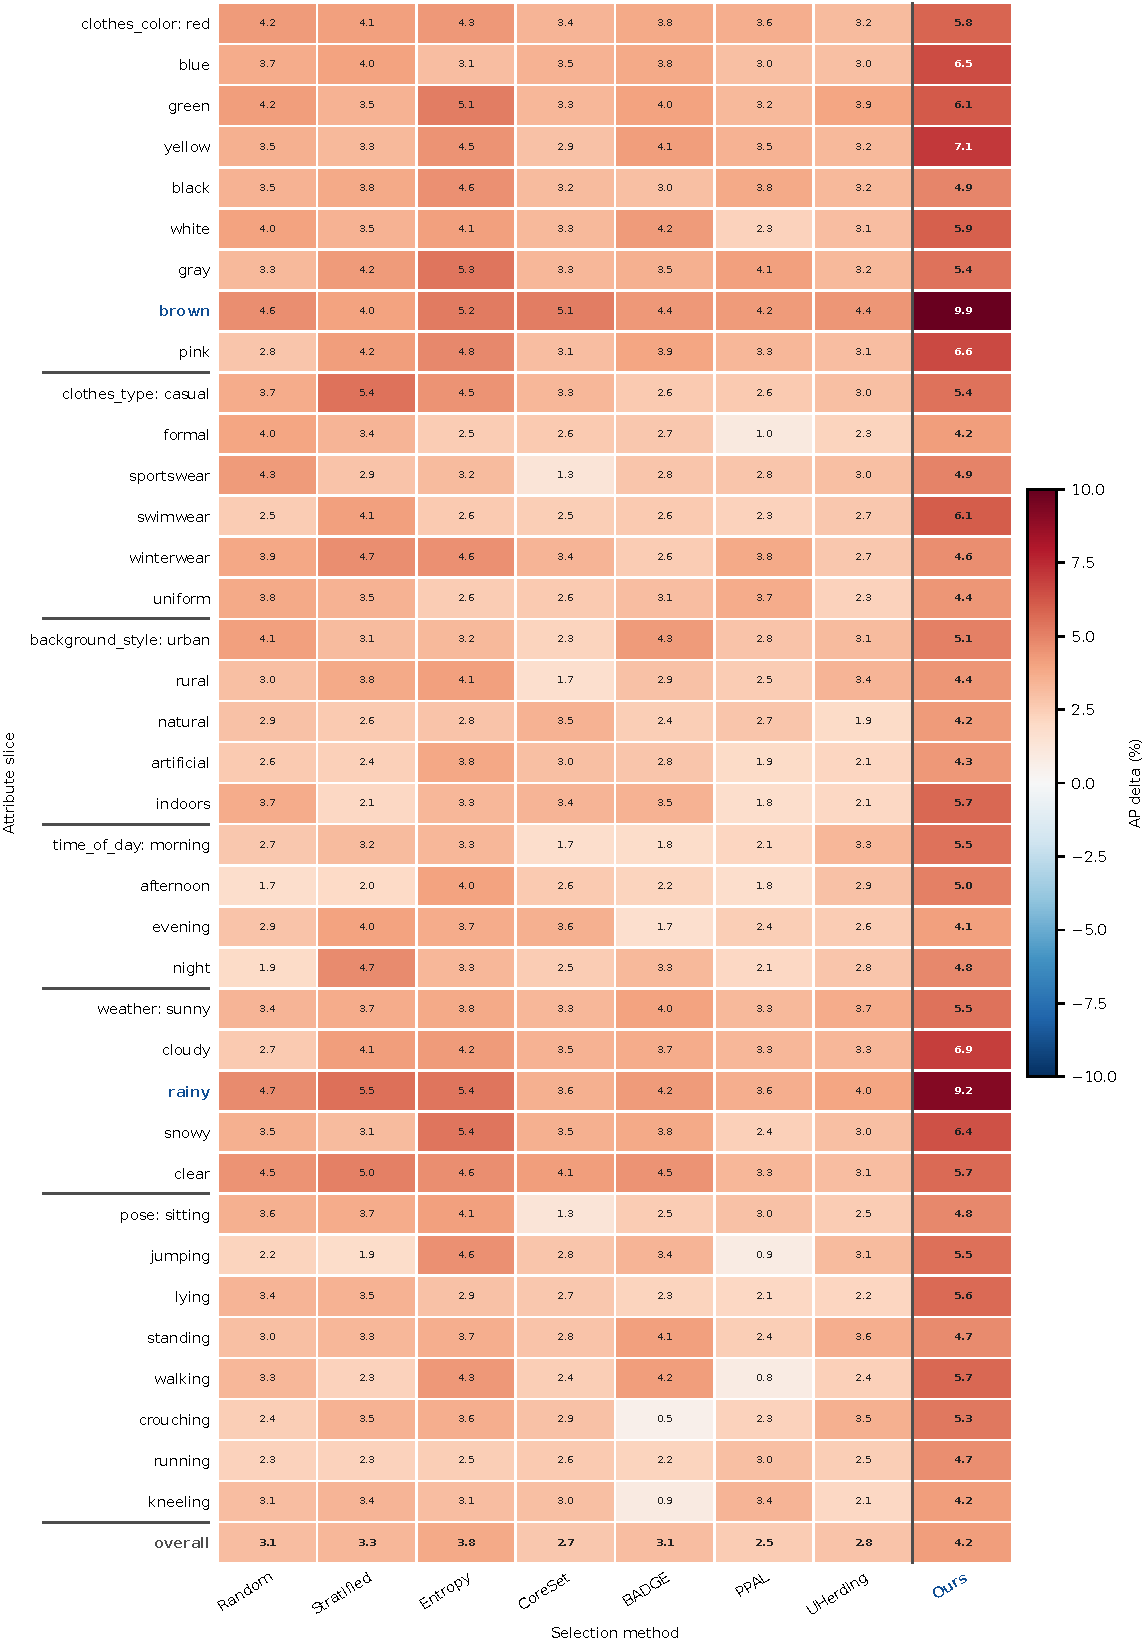
\includegraphics[width=\linewidth]{figures/show/coco_ratio0p5_show_heatmap.pdf}
\caption{COCO pose-estimation ratio-$0.5$ attribute-slice AP deltas. The figure expands the slice-level analysis to all annotated COCO pose-estimation attribute groups. The targeted repair values are clothes color brown and rainy weather.}
\label{fig:coco-ratio05-attribute-delta}
\end{figure}


\section{Effect of the VLM and Human Audit}
\label{app:vlm-human-audit}

\paragraph{VLM Role and Leakage Control}
\textbf{Where VLM annotations enter.}
\model uses the VLM as a fixed attribute annotator. Given a task-specific set of attribute fields and closed-set label options, the VLM assigns a discrete value to each image. The selector then uses these values, class labels, and generated-data attribute counts to choose the source subset. The repair-slice indicator is the binary conjunction of the target attribute values for the corresponding task: red hair, brown skin, and sad emotion for CelebA; pink color and fabric texture for ImageNet10; brown clothes and rainy weather for COCO; and red object color and cloudy weather for KITTI. The main repair metrics in Tables~\ref{tab:main-rer} and~\ref{tab:app-main-imagenet}--\ref{tab:app-main-kitti} are standard task metrics computed from benchmark labels, so the VLM does not grade the final repaired model. Test-set attributes are used only for post-training slice diagnostics.

\vspace{0.5em}
\textbf{Leakage control.}
The attribute vocabulary, target fields, and VLM annotation prompt are fixed before running the source-selection methods. The assignment stage does not receive model predictions, failure rates, method names, selected-set membership, or downstream results. In settings where the same VLM family is used for target-slice wording and image-level assignment, the two roles are still separated: the slice description is fixed first, and assignment is then run as a frozen closed-set classifier over images. Source selection uses only source-training attributes and generated-pool attributes. The relevant failure mode is inaccurate or self-consistent metadata rather than test-label leakage. The audit below tests the target fields with independent human labels.

\paragraph{Human Audit Protocol}
We conduct a blinded human audit with five AI graduate students. Each annotator labels 100 CelebA images, 100 COCO images, and 100 KITTI images using the same closed-set options as the VLM. Annotators see only the image, dataset name, and sample identifier; they do not see VLM labels, target flags, model predictions, data split, or method outputs. We aggregate human labels by majority vote and compare them with the VLM labels at two levels: exact agreement on the audited fields and binary agreement on the repair-slice indicator after applying the target values for those fields. For example, the COCO slice indicator is true only when the audited image has brown clothes and rainy weather, and the KITTI indicator is true only when it has red object color and cloudy weather. For CelebA, the indicator uses the full repair conjunction over red hair, brown skin, and sad emotion, rather than a single field such as hair color alone. The binary agreement is the most relevant check for \model because the selector uses these attributes to identify repair-relevant source examples.

\begin{table*}[t]
\centering
\caption{Human audit of VLM-assigned attributes. Five AI graduate students label each audited image using the same closed-set options as the VLM. Exact field agreement measures agreement on the audited attribute values, while slice-indicator agreement measures agreement on the binary target conjunction used for repair.}
\label{tab:vlm-human-audit}
\small
\setlength{\tabcolsep}{3pt}
\begin{tabular}{p{0.14\linewidth} C{0.27\linewidth} C{0.27\linewidth} C{0.22\linewidth}}
\toprule
\rowcolor{sectiongray} \textbf{Dataset} & \textbf{Target field 1 agree.} & \textbf{Target field 2 agree.} & \textbf{Slice-indicator agree.} \\
\midrule
CelebA & Hair color: 98\% & Skin tone: 99\% & 92\% \\
COCO & Clothes color: 97\% & Weather: 91\% & 90\% \\
KITTI & Object color: 98\% & Weather: 96\% & 94\% \\
\bottomrule
\end{tabular}
\end{table*}

The audit is designed to measure agreement rather than to estimate the prevalence of rare target conjunctions. As shown in Table~\ref{tab:vlm-human-audit}, the VLM and human consensus usually agree on the audited target fields and on the resulting binary slice indicators. This supports the use of the VLM as a scalable attribute annotator rather than as an oracle: the VLM provides metadata, and the human audit checks that the target fields used for repair are visually grounded.

\paragraph{Sensitivity to attribute noise.}
We also test whether \model is brittle to noisy attributes. For each audited dataset and each target field, we independently corrupt a fraction $p$ of VLM labels by replacing the original value with a different valid value from the same field vocabulary. We then rerun source selection with the corrupted attributes while keeping the generated repair set, source ratio, and training recipe fixed. Let $M_{\mathrm{clean}}$ and $M_{\mathrm{noisy}}$ denote the resulting task metrics at source ratio $0.5$, measured in the native $[0,1]$ scale. We report the absolute metric drop
\begin{equation}
\Delta = M_{\mathrm{clean}} - M_{\mathrm{noisy}}.
\end{equation}
Thus, positive values indicate that attribute corruption lowers performance, while a negative value would indicate an improvement under noise. Table~\ref{tab:attribute-noise-sensitivity} reports this drop for CelebA, COCO, and KITTI. The entries are absolute metric units: $0.007$ corresponds to a $0.7$ percentage-point drop, and $0.09$ corresponds to a $9$ percentage-point drop, not a $9\%$ relative change. Small drops under moderate noise would indicate that the selector depends on the aggregate attribute distribution rather than on a small number of individual VLM decisions.

\begin{table*}[t]
\centering
\caption{Sensitivity to corrupted VLM attributes at source ratio $0.5$. Entries report the absolute metric drop $\Delta=M_{\mathrm{clean}}-M_{\mathrm{noisy}}$ in native $[0,1]$ metric units; positive values indicate lower performance after corruption. Multiply by 100 to obtain percentage points. These are absolute drops, not relative percentage changes or standard deviations.}
\label{tab:attribute-noise-sensitivity}
\small
\setlength{\tabcolsep}{5pt}
\begin{tabular}{l c c c c}
\toprule
\rowcolor{sectiongray} \textbf{Dataset} & \textbf{Metric drop ($\Delta$)} & \textbf{5\% noise} & \textbf{10\% noise} & \textbf{20\% noise} \\
\midrule
CelebA & Test ACC & 0.007 & 0.01 & 0.09 \\
COCO & Test AP & 0.002 & 0.003 & 0.02 \\
KITTI & Test mAP50--95 & 0.003 & 0.004 & 0.06 \\
\bottomrule
\end{tabular}
\end{table*}

At $5\%$ and $10\%$ corruption, the metric drops are small across all three datasets. At $20\%$ noise, the drops are larger on CelebA and KITTI because the corrupted rarity and frequency counts no longer describe the diagnosed repair slice reliably. The ranking then reflects both corrupted attribute values and the intact soft class-balance term, moving the selected subset toward noisy attribute sampling with soft stratification. COCO shows a smaller drop over the tested range, but these results do not distinguish between robustness from aggregate attribute statistics and robustness from correlated visual factors.

\section{Effect of the Repair Pipeline and Image Generation}
\label{app:image-generation-effect}

\subsection{Alternative Repair Pipeline}

The main experiments use a SafeFix-style upstream workflow. To test whether the source-selection result depends on that pipeline, we replace its generated repair set with a fixed HiBug-generated set on CelebA. All selectors share the diagnosis checkpoint, 80,000-image source pool, generated-image budget, source ratios, retraining configuration, and five seeds. Only the source-selection rule changes.

\begin{table*}[t]
\centering
\caption{CelebA repair results with the HiBug repair pipeline. Metric: five-seed mean RER (\%).}
\label{tab:celeba-hibug-rer}
\footnotesize
\setlength{\tabcolsep}{3pt}
\begin{tabular}{c c c c c c c c >{\columncolor{myblue!8}}c}
\toprule
\rowcolor{sectiongray} \textbf{Ratio} & \textbf{Random} & \textbf{Stratified} & \textbf{Entropy} & \textbf{CoreSet} & \textbf{BADGE} & \textbf{UHerding} & \textbf{PPAL} & \cellcolor{myblue!8}\textbf{Ours} \\
\midrule
0.1 & 4.59 & 2.33 & 6.92 & -6.20 & 2.87 & -1.36 & 5.58 & \textbf{7.36} \\
0.3 & 5.91 & 5.08 & 8.02 & 7.79 & 1.66 & 3.39 & 3.87 & \textbf{8.07} \\
0.5 & 5.76 & 7.70 & 7.48 & 7.90 & 2.53 & 2.13 & 9.64 & \textbf{12.54} \\
0.7 & 2.57 & 8.06 & 10.03 & 6.19 & 7.86 & 4.96 & 5.90 & \textbf{11.16} \\
0.9 & 2.84 & 4.28 & 7.95 & 5.71 & 5.80 & 4.19 & 6.37 & \textbf{13.42} \\
\bottomrule
\end{tabular}
\end{table*}

\model has the highest RER at all five ratios. Its margins over the strongest baseline are $0.44/0.05/2.90/1.13/5.47$ RER points, or 2.00 points on average. This comparison is internal to the HiBug table: changing the upstream repair pipeline changes the generated set and can shift every selector's absolute RER.

\subsection{Alternative Image Generators}

The upstream workflow following \safefix~\citep{xu2025safefix} uses \controlnet~\citep{zhang2023adding} as the conditional diffusion model. The quality of diffusion-based dataset augmentation can vary with the generator and editing procedure~\citep{trabucco2023effective,dunlap2023diversify,wang2024domain}. To test whether \model depends on this particular generator, we replace \controlnet while keeping the rest of the repair pipeline fixed: InstructPix2Pix~\citep{brooks2023instructpix2pix} for CelebA and ICEdit~\citep{zhang2025icedit} for COCO.

Table~\ref{tab:celeba-instructpix2pix-rer} reports CelebA results with InstructPix2Pix generation. \model remains the strongest source selector at every active source ratio. Its absolute RER is lower than the corresponding \controlnet result in Table~\ref{tab:main-rer}, and the same decrease appears across the other selectors. This shared decrease is consistent with a generator-level effect rather than a change in the source-selection rule.

\begin{table*}[t]
\centering
\caption{CelebA repair results with InstructPix2Pix generation. Metric: RER (\%).}
\label{tab:celeba-instructpix2pix-rer}
\scriptsize
\setlength{\tabcolsep}{1.5pt}
\begin{tabular}{c c c c c c c c >{\columncolor{myblue!8}}c | >{\columncolor{myblue!8}}c}
\toprule
\rowcolor{sectiongray} \textbf{Ratio} & \textbf{Random} & \textbf{Stratified} & \textbf{Entropy} & \textbf{CoreSet} & \textbf{BADGE} & \textbf{UHerding} & \textbf{PPAL} & \cellcolor{myblue!8}\shortstack{\textbf{Ours}\\\textbf{(InstructPix2Pix)}} & \cellcolor{myblue!8}\shortstack{\textbf{Ours}\\\textbf{(ControlNet)}} \\
\midrule
0.1 & 4.23 & 1.95 & 6.41 & -6.65 & 2.34 & -1.78 & 5.12 & \textbf{7.65} & 8.48 \\
0.3 & 5.34 & 4.72 & 7.98 & 7.21 & 1.02 & 2.81 & 3.45 & \textbf{8.12} & 10.50 \\
0.5 & 5.56 & 7.23 & 6.78 & 7.54 & 2.12 & 1.56 & 9.12 & \textbf{11.17} & 13.79 \\
0.7 & 2.12 & 7.67 & 9.34 & 5.78 & 7.34 & 4.23 & 5.34 & \textbf{12.13} & 12.09 \\
0.9 & 2.45 & 3.92 & 7.56 & 5.34 & 5.23 & 3.87 & 5.91 & \textbf{13.87} & 14.74 \\
\bottomrule
\end{tabular}
\end{table*}

Table~\ref{tab:coco-icedit-rer} reports the corresponding COCO result with ICEdit. ICEdit improves the absolute RER values for most source ratios, and \model remains the best selector under this generator as well. These comparisons should be read horizontally: for a fixed generator and generated repair set, \model is compared against the non-attribute active-learning selectors. Changes in generator quality can shift the absolute repair numbers, but they do not remove the benefit of attribute-driven source selection.

\begin{table*}[t]
\centering
\caption{COCO pose-estimation repair results with ICEdit generation. Metric: RER (\%).}
\label{tab:coco-icedit-rer}
\scriptsize
\setlength{\tabcolsep}{1.5pt}
\begin{tabular}{c c c c c c c c >{\columncolor{myblue!8}}c | >{\columncolor{myblue!8}}c}
\toprule
\rowcolor{sectiongray} \textbf{Ratio} & \textbf{Random} & \textbf{Stratified} & \textbf{Entropy} & \textbf{CoreSet} & \textbf{BADGE} & \textbf{UHerding} & \textbf{PPAL} & \cellcolor{myblue!8}\shortstack{\textbf{Ours}\\\textbf{(ICEdit)}} & \cellcolor{myblue!8}\shortstack{\textbf{Ours}\\\textbf{(ControlNet)}} \\
\midrule
0.1 & 3.78 & 5.23 & 5.87 & -0.34 & 2.34 & 3.12 & 1.56 & \textbf{7.12} & 6.86 \\
0.3 & 3.92 & 8.67 & 8.12 & 9.12 & 6.56 & 4.67 & 6.89 & \textbf{10.34} & 9.86 \\
0.5 & 7.91 & 8.45 & 9.67 & 6.91 & 7.82 & 6.54 & 7.23 & \textbf{10.67} & 10.13 \\
0.7 & 6.54 & 10.12 & 9.98 & 9.56 & 9.12 & 6.71 & 8.23 & \textbf{10.87} & 10.18 \\
0.9 & 5.12 & 9.87 & 6.98 & 7.82 & 8.12 & 7.54 & 10.12 & \textbf{11.56} & 11.05 \\
\bottomrule
\end{tabular}
\end{table*}

\section{Additional Robustness and Sensitivity Studies}
\label{app:additional-robustness}

\subsection{Repair-Schedule Sensitivity}

The main ImageNet10 repair schedule uses 15 epochs, half of the 30-epoch diagnosis schedule. We vary repair training from 15 to 60 epochs at source ratios $0.5$ and $0.9$ while holding the diagnosis checkpoint, generated repair set, source budget, learning rate, and five seeds fixed. Table~\ref{tab:repair-schedule-sensitivity} reports the results.

\begin{table*}[t]
\centering
\caption{ImageNet10 repair-schedule sensitivity. Metric: five-seed mean RER (\%). We evaluate source ratios $0.5$ and $0.9$ across repair training schedules from 15 to 60 epochs ($0.5\times$--$2.0\times$ the 30-epoch diagnosis schedule), holding the diagnosis checkpoint, generated repair set, source budget, learning rate, and five seeds fixed.}
\label{tab:repair-schedule-sensitivity}
\small
\setlength{\tabcolsep}{6pt}
\begin{tabular}{c l c c c c}
\toprule
\rowcolor{sectiongray} \textbf{Ratio} & \textbf{Method} & \textbf{15 epochs ($0.5\times$)} & \textbf{30 epochs ($1.0\times$)} & \textbf{45 epochs ($1.5\times$)} & \textbf{60 epochs ($2.0\times$)} \\
\midrule
\multirow{8}{*}{0.5} 
& Random & 7.19 & 8.91 & 9.91 & 10.15 \\
& Stratified & 9.54 & 9.31 & 10.37 & 10.94 \\
& Entropy & 5.45 & 10.45 & 10.96 & 11.55 \\
& CoreSet & 7.90 & 9.86 & 10.09 & 11.44 \\
& BADGE & 10.35 & 10.62 & 11.72 & 11.99 \\
& UHerding & 8.23 & 8.81 & 9.18 & 10.05 \\
& PPAL & 8.72 & 9.16 & 10.22 & 10.44 \\
& \textbf{Ours} & \textbf{11.72} & \textbf{12.27} & \textbf{13.39} & \textbf{13.95} \\
\midrule
\multirow{8}{*}{0.9} 
& Random & 10.08 & 10.90 & 12.03 & 11.41 \\
& Stratified & 10.35 & 11.93 & 12.79 & 13.10 \\
& Entropy & 10.08 & 12.21 & 13.32 & 13.64 \\
& CoreSet & 5.99 & 11.96 & 12.19 & 13.27 \\
& BADGE & 9.26 & 9.93 & 10.97 & 11.36 \\
& UHerding & 11.44 & 11.99 & 12.25 & 12.48 \\
& PPAL & 11.72 & 12.07 & 12.69 & 12.89 \\
& \textbf{Ours} & \textbf{13.62} & \textbf{14.13} & \textbf{14.87} & \textbf{15.10} \\
\bottomrule
\end{tabular}
\end{table*}

Extending repair training from 15 to 60 epochs raises \model ACC from $0.7508$ to $0.7571$ at ratio $0.5$ and from $0.7562$ to $0.7603$ at ratio $0.9$. Relative to the pre-repair ACC of $0.7177$, the 60-epoch results correspond to gains of $3.94$ and $4.26$ percentage points, respectively. Over the same schedules, \model RER increases from $11.72\%$ to $13.95\%$ and from $13.62\%$ to $15.10\%$. Most baselines also improve overall, although individual trajectories are not strictly monotonic. \model is best in all eight ratio--epoch configurations, leading the strongest baseline by $1.37$--$1.96$ RER points at ratio $0.5$ and $1.46$--$1.92$ points at ratio $0.9$. The persistent ordering supports a selected-set quality effect rather than an early-stopping artifact.

\subsection{Slice-Granularity Sensitivity}

Slice granularity changes both the fields used for source selection and the generated repair set. We compare the diagnosed two-field conjunction with single-field variants and a narrower three-field conjunction over five seeds in Tables~\ref{tab:coco-slice-granularity} and~\ref{tab:imagenet-slice-granularity}.

\begin{table*}[t]
\centering
\caption{Slice-granularity sensitivity on COCO. Metric: keypoint AP. The diagnosed slice is brown clothes and rainy weather.}
\label{tab:coco-slice-granularity}
\small
\setlength{\tabcolsep}{4pt}
\begin{tabular}{c c c c >{\columncolor{myblue!8}}c}
\toprule
\rowcolor{sectiongray} \textbf{Ratio} & \textbf{Brown only} & \textbf{Rain only} & \textbf{Brown+rain+night} & \cellcolor{myblue!8}\textbf{Brown+rain} \\
\midrule
0.1 & 0.6161 & 0.6174 & 0.6097 & \textbf{0.6183} \\
0.3 & 0.6238 & 0.6224 & 0.6179 & \textbf{0.6306} \\
0.5 & 0.6284 & 0.6217 & 0.6246 & \textbf{0.6317} \\
0.7 & 0.6327 & \textbf{0.6333} & 0.6291 & 0.6319 \\
0.9 & 0.6348 & 0.6132 & 0.6336 & \textbf{0.6355} \\
\bottomrule
\end{tabular}
\end{table*}

\begin{table*}[t]
\centering
\caption{Slice-granularity sensitivity on ImageNet10. Metric: test accuracy. The diagnosed slice is pink color and fabric texture.}
\label{tab:imagenet-slice-granularity}
\small
\setlength{\tabcolsep}{4pt}
\begin{tabular}{c c c c >{\columncolor{myblue!8}}c}
\toprule
\rowcolor{sectiongray} \textbf{Ratio} & \textbf{Pink only} & \textbf{Fabric only} & \textbf{Pink+fabric+rainy background} & \cellcolor{myblue!8}\textbf{Pink+fabric} \\
\midrule
0.1 & 0.7223 & 0.7346 & \textbf{0.7398} & 0.7369 \\
0.3 & 0.7369 & 0.7431 & 0.7414 & \textbf{0.7492} \\
0.5 & 0.7377 & 0.7438 & 0.7429 & \textbf{0.7508} \\
0.7 & 0.7485 & 0.7423 & 0.7462 & \textbf{0.7515} \\
0.9 & 0.7500 & 0.7354 & 0.7491 & \textbf{0.7562} \\
\bottomrule
\end{tabular}
\end{table*}

The diagnosed two-field slice is best in 8 of the 10 dataset--ratio settings. On average, it exceeds COCO Brown-only, Rain-only, and the three-field slice by 0.24, 0.80, and 0.66 AP points. On ImageNet10, it exceeds Pink-only, Fabric-only, and the three-field slice by 0.98, 0.91, and 0.50 accuracy points. These results indicate a support--specificity trade-off: a single-field slice can mix different failure causes, while a narrow conjunction can remove useful support.

\subsection{Incomplete Attribute-Vocabulary Coverage}

Tables~\ref{tab:imagenet-missing-field} and~\ref{tab:coco-missing-field} report results after removing one target field while holding the generated repair pool, source budget, checkpoint, and training schedule fixed. Parenthesized values are the selected-set Jaccard overlap with the full two-field selector.

\begin{table*}[t]
\centering
\caption{Missing-field sensitivity on ImageNet10. Metric: overall test accuracy (\%).}
\label{tab:imagenet-missing-field}
\small
\setlength{\tabcolsep}{5pt}
\begin{tabular}{c >{\columncolor{myblue!8}}c c c}
\toprule
\rowcolor{sectiongray} \textbf{Ratio} & \cellcolor{myblue!8}\textbf{Full} & \textbf{Missing color} & \textbf{Missing texture} \\
\midrule
0.1 & 73.69 & 72.69 (0.5604) & \textbf{73.85} (0.3904) \\
0.3 & \textbf{74.92} & 73.77 (0.6166) & 73.54 (0.5842) \\
0.5 & \textbf{75.08} & 74.23 (0.6443) & 74.23 (0.7330) \\
0.7 & \textbf{75.15} & 74.00 (0.6999) & 74.23 (0.8826) \\
0.9 & \textbf{75.62} & 75.08 (0.8765) & 74.54 (0.9668) \\
\bottomrule
\end{tabular}
\end{table*}

\begin{table*}[t]
\centering
\caption{Missing-field sensitivity on COCO. Metric: keypoint AP.}
\label{tab:coco-missing-field}
\small
\setlength{\tabcolsep}{5pt}
\begin{tabular}{c >{\columncolor{myblue!8}}c c c}
\toprule
\rowcolor{sectiongray} \textbf{Ratio} & \cellcolor{myblue!8}\textbf{Full} & \textbf{Missing color} & \textbf{Missing weather} \\
\midrule
0.1 & \textbf{0.6183} & 0.6055 (0.4782) & 0.6105 (0.2034) \\
0.3 & \textbf{0.6306} & 0.6221 (0.5611) & 0.6214 (0.4613) \\
0.5 & \textbf{0.6317} & 0.6178 (0.7063) & 0.6271 (0.6084) \\
0.7 & 0.6319 & \textbf{0.6332} (0.7836) & 0.6323 (0.8110) \\
0.9 & \textbf{0.6355} & 0.6237 (0.8969) & 0.6244 (0.8708) \\
\bottomrule
\end{tabular}
\end{table*}

Missing-field variants are lower than Full in 17 of the 20 dataset--field--ratio comparisons. The selected subset changes most at low budgets: at ratio $0.1$, Jaccard overlap falls as low as 0.3904 on ImageNet10 and 0.2034 on COCO. Mean ImageNet10 accuracy changes are $-0.94/-0.81$ points when color/texture is removed; mean COCO AP changes are $-0.0091/-0.0065$ when color/weather is removed. The effect is not monotonic at every ratio, but incomplete coverage usually weakens task performance.

\section{Source-Only Data Selection}
\label{app:source-only-selection}

We evaluate \model outside model repair on ImageNet10. These experiments use no generated images, diagnosed slices, or repair checkpoints. A fresh ResNet-18 is trained on each selected subset, and every result is a five-seed mean. In this setting, because no generated data is present ($\tilde{n}_a^{\mathrm{gen}}(v)=0$), \model retains the source-distribution head-value term of the frequency penalty, as shown in Eq.~\ref{eq:source-only-base-score} in Appendix~\ref{app:no-generation-corner-case}. The resulting score combines this term with group-conditional rarity and soft class balancing.

\subsection{One-Shot Subset Selection}

We add two direct semantic baselines. \textbf{Attribute Rarity} is a frequency-penalty ablation that ranks images by class-conditional rarity of their assigned attribute values and applies soft class balancing. \textbf{Semantic CoreSet} one-hot encodes the assigned values and runs class-balanced greedy $k$-center selection in that semantic representation.

\begin{table*}[t]
\centering
\caption{ImageNet10 source-only one-shot data selection. Metric: five-seed mean test accuracy (\%).}
\label{tab:source-only-one-shot}
\small
\setlength{\tabcolsep}{3pt}
\resizebox{\linewidth}{!}{%
\begin{tabular}{c c c c c c c c >{\columncolor{myblue!8}}c}
\toprule
\rowcolor{sectiongray} \textbf{Ratio} & \textbf{Random} & \textbf{Stratified} & \textbf{Entropy} & \textbf{CoreSet} & \textbf{BADGE} & \textbf{Attribute rarity} & \textbf{Semantic CoreSet} & \cellcolor{myblue!8}\textbf{Ours} \\
\midrule
0.1 & 43.23 & 41.85 & 26.86 & 38.32 & 42.62 & 44.46 & 44.08 & \textbf{45.00} \\
0.3 & 55.83 & 57.15 & 44.63 & 56.15 & 58.17 & 56.54 & 56.55 & \textbf{58.32} \\
0.5 & 64.77 & 64.14 & 58.69 & 64.86 & 63.18 & 65.31 & 62.55 & \textbf{66.52} \\
0.7 & 69.46 & 71.63 & 66.71 & 68.03 & 69.57 & 71.00 & 67.18 & \textbf{72.02} \\
0.9 & 71.34 & 71.69 & 72.88 & 72.89 & 72.38 & 72.48 & 71.23 & \textbf{72.92} \\
\bottomrule
\end{tabular}%
}
\end{table*}

\model has the highest accuracy at all five budgets. Its margins over the strongest alternative are $0.54/0.15/1.21/0.39/0.03$ accuracy points at ratios $0.1/0.3/0.5/0.7/0.9$.

\subsection{Iterative Active Learning}

All methods start from the same labeled set at ratio $0.1$ and add labeled data over five acquisition rounds. Object--Attribute Entropy Reduction adapts the object--attribute query criterion to the setting in which attributes are already known and only the class label is queried.

\begin{table*}[t]
\centering
\caption{ImageNet10 source-only iterative active learning. Metric: five-seed mean test accuracy (\%); Curve Mean averages ratios $0.1$--$0.6$.}
\label{tab:source-only-active-learning}
\small
\setlength{\tabcolsep}{3pt}
\resizebox{\linewidth}{!}{%
\begin{tabular}{c c c c c c c >{\columncolor{myblue!8}}c}
\toprule
\rowcolor{sectiongray} \textbf{Ratio} & \textbf{Random} & \textbf{Entropy} & \textbf{CoreSet} & \textbf{BADGE} & \textbf{Attribute rarity} & \textbf{Object--attribute entropy} & \cellcolor{myblue!8}\textbf{Ours-AL} \\
\midrule
0.1 & 43.23 & 43.23 & 43.23 & 43.23 & 43.23 & 43.23 & 43.23 \\
0.2 & 51.11 & \textbf{52.26} & 50.00 & 51.26 & 50.92 & 50.48 & 51.32 \\
0.3 & 55.38 & 54.85 & 55.00 & 56.17 & 52.94 & 55.95 & \textbf{56.95} \\
0.4 & 58.71 & 58.63 & 59.54 & 60.46 & 60.46 & 60.31 & \textbf{63.02} \\
0.5 & 61.97 & 63.69 & 63.92 & 61.89 & 61.86 & 63.88 & \textbf{65.18} \\
0.6 & 66.15 & 66.69 & 68.15 & 67.11 & 65.78 & 65.78 & \textbf{68.80} \\
\midrule
Curve Mean & 56.09 & 56.56 & 56.64 & 56.69 & 55.87 & 56.61 & \textbf{58.08} \\
\bottomrule
\end{tabular}%
}
\end{table*}

\modelplain-AL is strongest from ratios $0.3$ through $0.6$ and improves Curve Mean by 1.39 points over BADGE. The source-only comparison shows that the selection rule is not tied to checkpoint fine-tuning or a generated repair set.

\subsection{Alternative Attribute Sources}

We repeat the source-only evaluation with Qwen3-VL, BLIP, and InternVL3 assignments under the same closed-set vocabulary, training protocol, and five seeds.

\begin{table*}[t]
\centering
\caption{Sensitivity to the attribute source. One-Shot Mean averages ratios $0.1/0.3/0.5/0.7/0.9$; AL Curve Mean averages ratios $0.1$--$0.6$.}
\label{tab:attribute-source-ablation}
\small
\setlength{\tabcolsep}{6pt}
\begin{tabular}{l c c c}
\toprule
\rowcolor{sectiongray} \textbf{Attribute source} & \textbf{One-Shot Mean} & \textbf{AL Curve Mean} & \textbf{Final ACC at 0.6} \\
\midrule
Qwen3-VL & 62.96 & \textbf{58.08} & \textbf{68.80} \\
BLIP & 62.18 & 55.99 & 65.46 \\
InternVL3 & \textbf{63.27} & 56.33 & 66.23 \\
\bottomrule
\end{tabular}
\end{table*}

No attribute source is strongest in both settings. InternVL3 has the highest One-Shot Mean, 0.31 points above Qwen3-VL. Qwen3-VL is strongest in active learning, exceeding InternVL3 by 1.75 points in Curve Mean and 2.57 points at ratio $0.6$. The method works with all three sources, but annotation quality and representation affect the selected subset and downstream result.

\section{Additional Theory Analysis}
\label{app:theory-analysis}

\paragraph{Proof of conditional target-slice enrichment}
The result concerns a fixed source pool and a fixed group allocation $B_c$. For $x_i\in T_c$ and $x_j\notin T_c$, attributes with $v_{i,a}=v_{j,a}$ cancel from both score components. With $\mathcal{D}_{ij}=\{a\in\selattrs:v_{i,a}\neq v_{j,a}\}$, the differences in Proposition~\ref{prop:rarity-margin} are
\begin{align}
A_{ij}
&=\sum_{a\in\mathcal{D}_{ij}}
\left[(n_a(v_{i,a}\mid c)+\varepsilon)^{-\alpha}
-(n_a(v_{j,a}\mid c)+\varepsilon)^{-\alpha}\right],\label{eq:rarity-advantage}\\
F_{ij}
&=\sum_{a\in\mathcal{D}_{ij}}
\frac{\hat n_a(v_{i,a})-\hat n_a(v_{j,a})}
{\sum_{v\in\vals_a}\hat n_a(v)}.\label{eq:frequency-disadvantage}
\end{align}
These conditions concern marginal attribute counts. A small joint support $|T_c|$ does not imply $A_{ij}>0$.

\begin{tcolorbox}[
    colback=green!2!white,
    colframe=green!20!white,
    arc=3pt,
    boxrule=1pt,
    drop shadow,
    breakable
]
\begin{proof}[Proof of Proposition~\ref{prop:rarity-margin}]
For each target/non-target pair in group $c$, Eqs.~\ref{eq:rarity-term}--\ref{eq:base-attribute-score} give
\begin{align}
\bar{s}_i-\bar{s}_j
&=\sum_{a\in\selattrs}(R_{i,a}-R_{j,a})\notag\\
&\quad-\lambda\sum_{a\in\selattrs}
\frac{\hat n_a(v_{i,a})-\hat n_a(v_{j,a})}
{\sum_{v\in\vals_a}\hat n_a(v)}\notag\\
&=A_{ij}-\lambda F_{ij}.\label{eq:base-score-gap}
\end{align}
When $F_{ij}\leq0$, the assumed $A_{ij}>0$ yields
\begin{equation*}
\bar{s}_i-\bar{s}_j=A_{ij}-\lambda F_{ij}\geq A_{ij}>0.
\end{equation*}
When $F_{ij}>0$, $\lambda<\lambda_c^\star\leq A_{ij}/F_{ij}$ yields
\begin{equation*}
\bar{s}_i-\bar{s}_j
=F_{ij}\left(\frac{A_{ij}}{F_{ij}}-\lambda\right)>0.
\end{equation*}
At every greedy step $k$, candidates in group $c$ receive the same balance bonus, so
\begin{align*}
\tilde{s}_i^{(k)}-\tilde{s}_j^{(k)}
&=\big(\bar{s}_i+C_c^{(k)}\big)-\big(\bar{s}_j+C_c^{(k)}\big)\\
&=\bar{s}_i-\bar{s}_j>0.
\end{align*}
Thus all target examples precede non-target examples in the group-$c$ queue. The first $B_c$ selections from that queue contain
\begin{align*}
|\dataset_{\mathrm{sel}}^{\mathrm{src}}\cap T_c|
&=\begin{cases}
B_c,& B_c\leq |T_c|,\\
|T_c|,& B_c>|T_c|
\end{cases}\\
&=\min\{B_c,|T_c|\}.
\end{align*}
For a uniform random draw of $B_c$ examples from the same $N_c$-element group, each source example has inclusion probability $B_c/N_c$. Consequently,
\begin{equation*}
\mathbb{E}[|S_{\mathrm{rand}}\cap T_c|]
=\sum_{i\in T_c}\mathbb{P}(i\in S_{\mathrm{rand}})
=B_c\frac{|T_c|}{N_c}.
\end{equation*}
\end{proof}
\end{tcolorbox}

For $0<|T_c|<N_c$ and $0<B_c<N_c$, the conditional enrichment gap is strict:
\begin{equation*}
\min\{B_c,|T_c|\}-B_c\frac{|T_c|}{N_c}
=\begin{cases}
B_c(1-|T_c|/N_c),& B_c\leq|T_c|,\\
|T_c|(1-B_c/N_c),& B_c>|T_c|
\end{cases}>0.
\end{equation*}
This is a selection-count result for a fixed $B_c$. It does not establish that the algorithm assigns positive budget to group $c$, nor does it imply a gain in the trained model's task metric. The random comparison requires the same group allocation and uniform sampling within the group.

A rare conjunction may fail the pairwise condition. For example, if binary combinations $(A,B)=(1,1),(1,0),(0,1),(0,0)$ occur $1,49,49,1$ times, the target conjunction $(1,1)$ has $1\%$ support, but each defining marginal value occurs 50 times. Its marginal rarity score therefore does not strictly separate it from all non-target examples. The sufficient condition $A_{ij}>0$ must be checked for the actual selector fields and score parameters before applying the bound to a particular run.

\paragraph{Geometric coverage}
Let $q_c$ be the empirical $\epsilon$-covering number of $\{z_i:x_i\in T_c\}$ when centers must come from that set. Then $q_c$ target representatives suffice to cover the target slice at radius $\epsilon$. This local fact does not bound the number of target examples in a globally optimal fixed-budget $k$-center solution or in greedy CoreSet: target centers can also cover non-target points, and the global objective can favor additional target centers.

\paragraph{Finite-weight group balance}
Here $c$ denotes a selection group. At step $k$, let $H_c^{(k)}$ be the highest remaining base score in active group $c$ and define $\Delta_k=\max_c H_c^{(k)}-\min_c H_c^{(k)}$. The count $n_c^{(k)}$ is measured before the step.
\begin{tcolorbox}[
    colback=blue!2!white,
    colframe=blue!20!white,
    arc=3pt,
    boxrule=1pt,
    drop shadow,
    breakable
]
\begin{lemma}[Balance pressure at one selection step]
\label{lem:finite-weight-balance}
Assume $0<w<\infty$. If the selector chooses a candidate from group $d$ while group $c$ is also active, then
\begin{equation}
\label{eq:finite-balance-gap}
n_d^{(k)}-n_c^{(k)}\leq\frac{t\Delta_k}{w}.
\end{equation}
\end{lemma}
\end{tcolorbox}

\begin{tcolorbox}[
    colback=green!2!white,
    colframe=green!20!white,
    arc=3pt,
    boxrule=1pt,
    drop shadow,
    breakable
]
\begin{proof}
The chosen group's adjusted head score is at least that of group $c$. Hence
\begin{align*}
H_d^{(k)}+w\frac{t-n_d^{(k)}}{t}
&\geq H_c^{(k)}+w\frac{t-n_c^{(k)}}{t},\\
\frac{w}{t}\big(n_d^{(k)}-n_c^{(k)}\big)
&\leq H_d^{(k)}-H_c^{(k)}\\
&\leq\Delta_k.
\end{align*}
Dividing by $w/t>0$ gives Eq.~\ref{eq:finite-balance-gap}.
\end{proof}
\end{tcolorbox}

The bound applies to counts before the chosen step; it is not a final group-quota guarantee. In the limit $w\to\infty$, finite base scores make the selector choose among active groups with the smallest count. If every group has candidates throughout selection, this gives round-robin group counts differing by at most one. The group bonus is shared within each group, so it preserves that group's base-score ordering.

\subsection{No-Generation Corner Case}
\label{app:no-generation-corner-case}
When $\dataset_{\mathrm{gen}}=\emptyset$, $\tilde n_a^{\mathrm{gen}}(v)=0$ and $\hat n_a(v)=n_a^{\mathrm{src}}(v)$. The source-only score is
\begin{equation}
\label{eq:source-only-base-score}
\bar{s}_i
=\sum_{a\in\selattrs}
\left[
\left(n_a(v_{i,a}\mid g_i)+\varepsilon\right)^{-\alpha}
-\lambda\frac{n_a^{\mathrm{src}}(v_{i,a})}
{\sum_{v\in\vals_a}n_a^{\mathrm{src}}(v)}
\right].
\end{equation}
The second term now penalizes common source attribute values. Proposition~\ref{prop:rarity-margin} still applies if its pairwise score condition holds under these source-only counts. Source selection can only return examples already present in the source pool.

\section{Hyperparameter Details}
\label{app:hyperparameter-details}
Table~\ref{tab:rpc-hyperparameters} reports the \model hyperparameters used in the main experiments. The parameters are the rarity exponent $\alpha$, frequency-penalty weight $\lambda$, and soft group-balancing weight $w$, matching the notation in Eq.~\ref{eq:class-balance-score}. The effective generated-count scale $\gamma_r$ is specified by task and source ratio in Appendix~\ref{app:implementation-details}.

\begin{table*}[t]
\centering
\caption{\model hyperparameters used in the main experiments.}
\label{tab:rpc-hyperparameters}
\small
\setlength{\tabcolsep}{5pt}
\begin{tabular}{l c c c}
\toprule
\rowcolor{sectiongray} \textbf{Dataset} & $\boldsymbol{\alpha}$ & $\boldsymbol{\lambda}$ & \textbf{w} \\
\midrule
ImageNet10 & 0.03 & 0.5 & 15 \\
CelebA & 0.03 & 0.5 & 15 \\
COCO & 0.03 & 0.5 & 15 \\
KITTI & 0.01 & 5.0 & 15 \\
\bottomrule
\end{tabular}
\end{table*}

All four settings add 1k generated images, but KITTI has only 5,000 source training images, compared with 10,400 for ImageNet10, 20,000 for COCO, and 80,000 for CelebA. Because the generated images form a larger fraction of the KITTI repair pool, we use $\lambda=5.0$ for KITTI and $\lambda=0.5$ for the other datasets.

Table~\ref{tab:kitti-rpc-sensitivity} gives the KITTI sensitivity across source-selection ratios. Test mAP50--95 changes only modestly across the evaluated parameter settings once the generated-data frequency penalty is present.

\begin{table*}[t]
\centering
\caption{KITTI \model sensitivity. Metric: test mAP50--95.}
\label{tab:kitti-rpc-sensitivity}
\small
\setlength{\tabcolsep}{4pt}
\begin{tabular}{c c c c c c c c}
\toprule
\rowcolor{sectiongray} $\boldsymbol{\alpha}$ & $\boldsymbol{\lambda}$ & \textbf{w} & \textbf{0.1} & \textbf{0.3} & \textbf{0.5} & \textbf{0.7} & \textbf{0.9} \\
\midrule
0.01 & 5.0 & 15 & \textbf{0.5372} & \textbf{0.5646} & \textbf{0.5773} & 0.5780 & \textbf{0.5850} \\
0.03 & 0.5 & 15 & 0.5358 & 0.5637 & 0.5764 & 0.5774 & 0.5842 \\
0.03 & 5.0 & 8 & 0.5366 & 0.5641 & 0.5769 & \textbf{0.5784} & 0.5847 \\
0.10 & 5.0 & 15 & 0.5349 & 0.5640 & 0.5768 & 0.5776 & 0.5839 \\
0.80 & 10.0 & 4 & 0.5337 & 0.5629 & 0.5756 & 0.5769 & 0.5828 \\
\bottomrule
\end{tabular}
\end{table*}

Table~\ref{tab:coco-rpc-sensitivity} shows the same pattern on COCO pose-estimation repair. The selected main setting remains strongest for most ratios, while nearby \model parameter settings stay within a narrow AP band.

\begin{table*}[t]
\centering
\caption{COCO \model sensitivity. Metric: COCO keypoint AP.}
\label{tab:coco-rpc-sensitivity}
\small
\setlength{\tabcolsep}{4pt}
\begin{tabular}{c c c c c c c c}
\toprule
\rowcolor{sectiongray} $\boldsymbol{\alpha}$ & $\boldsymbol{\lambda}$ & \textbf{w} & \textbf{0.1} & \textbf{0.3} & \textbf{0.5} & \textbf{0.7} & \textbf{0.9} \\
\midrule
0.03 & 0.5 & 15 & \textbf{0.6183} & \textbf{0.6306} & \textbf{0.6317} & 0.6319 & \textbf{0.6355} \\
0.01 & 0.5 & 15 & 0.6152 & 0.6298 & 0.6309 & 0.6308 & 0.6337 \\
0.03 & 0.5 & 8 & 0.6165 & 0.6289 & 0.6305 & \textbf{0.6323} & 0.6344 \\
0.03 & 0.5 & 0 & 0.6148 & 0.6276 & 0.6292 & 0.6306 & 0.6328 \\
0.00 & 0.0 & 15 & 0.6042 & 0.6288 & 0.6203 & 0.6313 & 0.6268 \\
\bottomrule
\end{tabular}
\end{table*}

\section{COCO Pose-Estimation Attribute-Score Component Ablation}
\label{app:coco-rpc-ablation}

Table~\ref{tab:coco-rpc-ablation} reports the corresponding component ablation for COCO pose-estimation repair. The full $\textcolor{colorR}{R}+\textcolor{colorP}{P}+\textcolor{colorC}{C}$ setting is strongest at all five ratios. This pattern supports complementary roles for the three terms in the evaluated COCO repair settings.

\begin{table*}[t]
\centering
\caption{COCO pose-estimation attribute-score component ablation. Metric: COCO keypoint AP.}
\label{tab:coco-rpc-ablation}
\small
\setlength{\tabcolsep}{4pt}
\begin{tabular}{c c c c c c c c >{\columncolor{myblue!8}}c}
\toprule
\rowcolor{sectiongray} \textbf{Ratio} & \textbf{none} & $\textcolor{colorR}{\boldsymbol{R}}$ & $\textcolor{colorP}{\boldsymbol{P}}$ & $\textcolor{colorC}{\boldsymbol{C}}$ & $\textcolor{colorP}{\boldsymbol{P}}+\textcolor{colorC}{\boldsymbol{C}}$ & $\textcolor{colorR}{\boldsymbol{R}}+\textcolor{colorC}{\boldsymbol{C}}$ & $\textcolor{colorR}{\boldsymbol{R}}+\textcolor{colorP}{\boldsymbol{P}}$ & \cellcolor{myblue!8}$\textcolor{colorR}{\boldsymbol{R}}+\textcolor{colorP}{\boldsymbol{P}}+\textcolor{colorC}{\boldsymbol{C}}$ \\
\midrule
0.1 & 0.6048 & 0.6099 & 0.5983 & 0.6067 & 0.6066 & 0.6149 & 0.5954 & \textbf{0.6183} \\
0.3 & 0.6040 & 0.6134 & 0.6038 & 0.6136 & 0.6142 & 0.6196 & 0.6136 & \textbf{0.6306} \\
0.5 & 0.6209 & 0.6074 & 0.6113 & 0.6149 & 0.6295 & 0.6246 & 0.6155 & \textbf{0.6317} \\
0.7 & 0.6151 & 0.6222 & 0.6231 & 0.6309 & 0.6317 & 0.6302 & 0.6282 & \textbf{0.6319} \\
0.9 & 0.6091 & 0.6175 & 0.6174 & 0.6270 & 0.6276 & 0.6225 & 0.6231 & \textbf{0.6355} \\
\bottomrule
\end{tabular}
\end{table*}

The leave-one-component-out comparisons show that removing any term reduces average AP relative to the full score, with average drops ranging from $0.00724$ to $0.01444$ after averaging the five displayed ratios. The full score also exceeds every single-component variant at every ratio. Overall, the COCO ablation supports the same conclusion as ImageNet10: the best repair behavior comes from combining rarity, generated-data frequency control, and soft class balancing rather than relying on any one term alone.

\section{Selection t-SNE Visualizations}
\label{app:selection-tsne}

We visualize the selected subsets in a shared low-dimensional embedding space. These plots are qualitative: the t-SNE coordinates~\citep{van2008visualizing} are computed from lightweight image proxy embeddings and are used only for visualization. Gray points denote source candidates, and colored points denote the subset selected by each method.

The ratio-$0.10$ plots in Figures~\ref{fig:tsne-r01-coco} and~\ref{fig:tsne-r01-kitti} show the selected subsets for COCO and KITTI. The ratio-$0.05$ COCO pose-estimation plots in Figures~\ref{fig:tsne-r005-coco} and~\ref{fig:tsne-overlay-r005-coco} examine the selection under an aggressive source budget ($n=1{,}000$, $5\%$ of the candidate pool), directly matching the constrained-budget retraining evaluations in Table~\ref{tab:constrained-source-budget}. The overlay figure makes the spatial separation between \model and representative active-learning baselines straightforward to inspect.

The visual pattern should be interpreted in light of the selection score in Section~\ref{subsec:slice-enrichment}. \model is not designed to be a uniformly spread coreset in the t-SNE plane. It behaves more like an attribute-conditioned real-source search: the selected images are related to the repair attributes, but they are spread across more diverse backgrounds, classes, and nearby contexts. The rarity term $\textcolor{colorR}{R_{i,a}}$ intentionally gives higher priority to source examples whose attribute values are rare within their class, so \model can place more mass on peripheral or less common regions of the proxy embedding. These peripheral selections are consistent with the intended rare-case behavior, although the t-SNE plot alone should be read only as a qualitative diagnostic. The penalty term $\textcolor{colorP}{P_{i,a}}$ reduces the priority of attribute values already supplied by the generated pool, so the selected source points are encouraged to complement the synthetic repair data instead of repeating it. Finally, the soft class-balance correction $\textcolor{colorC}{C_c^{(k)}}$ pulls the greedy selection away from a single high-scoring class or local region. The expected pattern is controlled non-uniformity: \model may put more mass on visually or semantically unusual regions than random, uncertainty, or pure coverage baselines while retaining cross-class coverage through the balance term.

The COCO overlay in Figure~\ref{fig:tsne-overlay-r005-coco} and facet panels in Figure~\ref{fig:tsne-r005-coco} illustrate this qualitative behavior under severe resource constraints. Under this $5\%$ budget, all generic active-learning selectors incur performance degradation (test AP between $0.5693$ and $0.5827$, relative to the pre-repair base of $0.5902$) because they either sample central mass broadly (Random and Stratified), concentrate tightly on ambiguous high-entropy clusters (Entropy and BADGE), or force extreme geometric dispersion along the perimeter (CoreSet) without targeting the diagnosed repair slice. In contrast, \model is the only method achieving positive repair (test AP $0.5969$, RER $+1.63\%$). Spatially, its selections concentrate on attribute-relevant subregions (clothing color brown and rainy weather) while deploying points across less frequent attribute combinations along the manifold periphery. Because t-SNE is only a two-dimensional proxy visualization, these plots should not be interpreted as standalone proof that shifting points improves downstream repair. They instead provide a qualitative sanity check that \model is not visibly collapsing onto the same region as the standard active-learning selectors.

% \begin{figure}[p]
% \centering
% \includegraphics[width=\linewidth]{figures/ratio0p1_selection_tsne/imagenet_controlnet_ratio0p1_selection_tsne.png}
% \caption{ImageNet ratio-$0.10$ selected subsets visualized on a shared source-image t-SNE embedding. Gray points show source candidates; colored points show the subset selected by each method.}
% \label{fig:tsne-r01-imagenet}
% \end{figure}

% \begin{figure}[p]
% \centering
% \includegraphics[width=\linewidth]{figures/ratio0p1_selection_tsne/celeba_redhair_brownskin_sademotion_ratio0p1_selection_tsne.png}
% \caption{CelebA ratio-$0.10$ selected subsets visualized on a shared source-image t-SNE embedding.}
% \label{fig:tsne-r01-celeba}
% \end{figure}

\begin{figure*}[p]
\centering
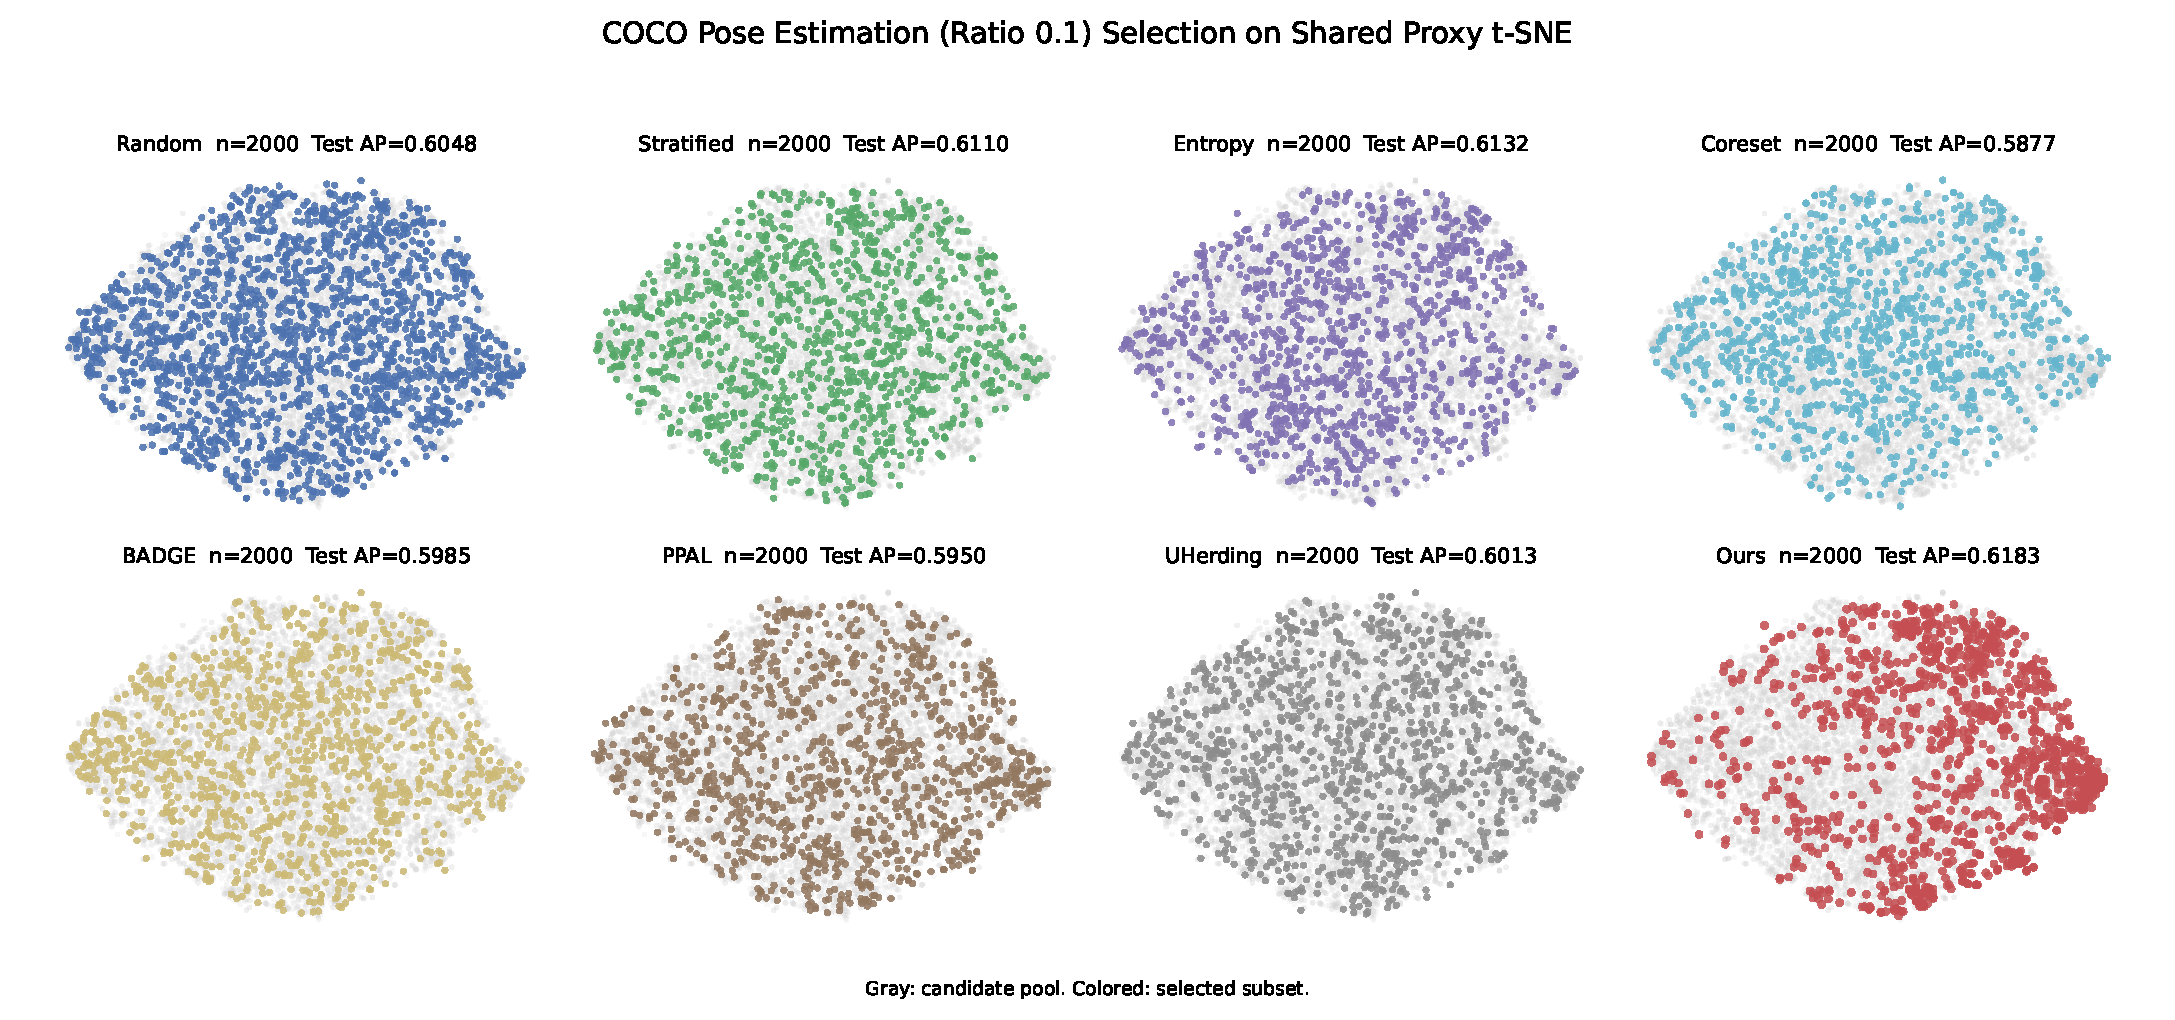
\includegraphics[width=\linewidth]{figures/ratio0p1_selection_tsne/coco_brown_rainy_ratio0p1_selection_tsne.pdf}
\caption{COCO pose-estimation ratio-$0.10$ selected subsets visualized on a shared source-image t-SNE embedding. Each method selects an identical source budget of $n=2{,}000$ training images from the $N=20{,}000$ candidate pool; for visual clarity, 12,000 randomly subsampled candidate points are displayed in the background.}
\label{fig:tsne-r01-coco}
\end{figure*}

\begin{figure*}[p]
\centering
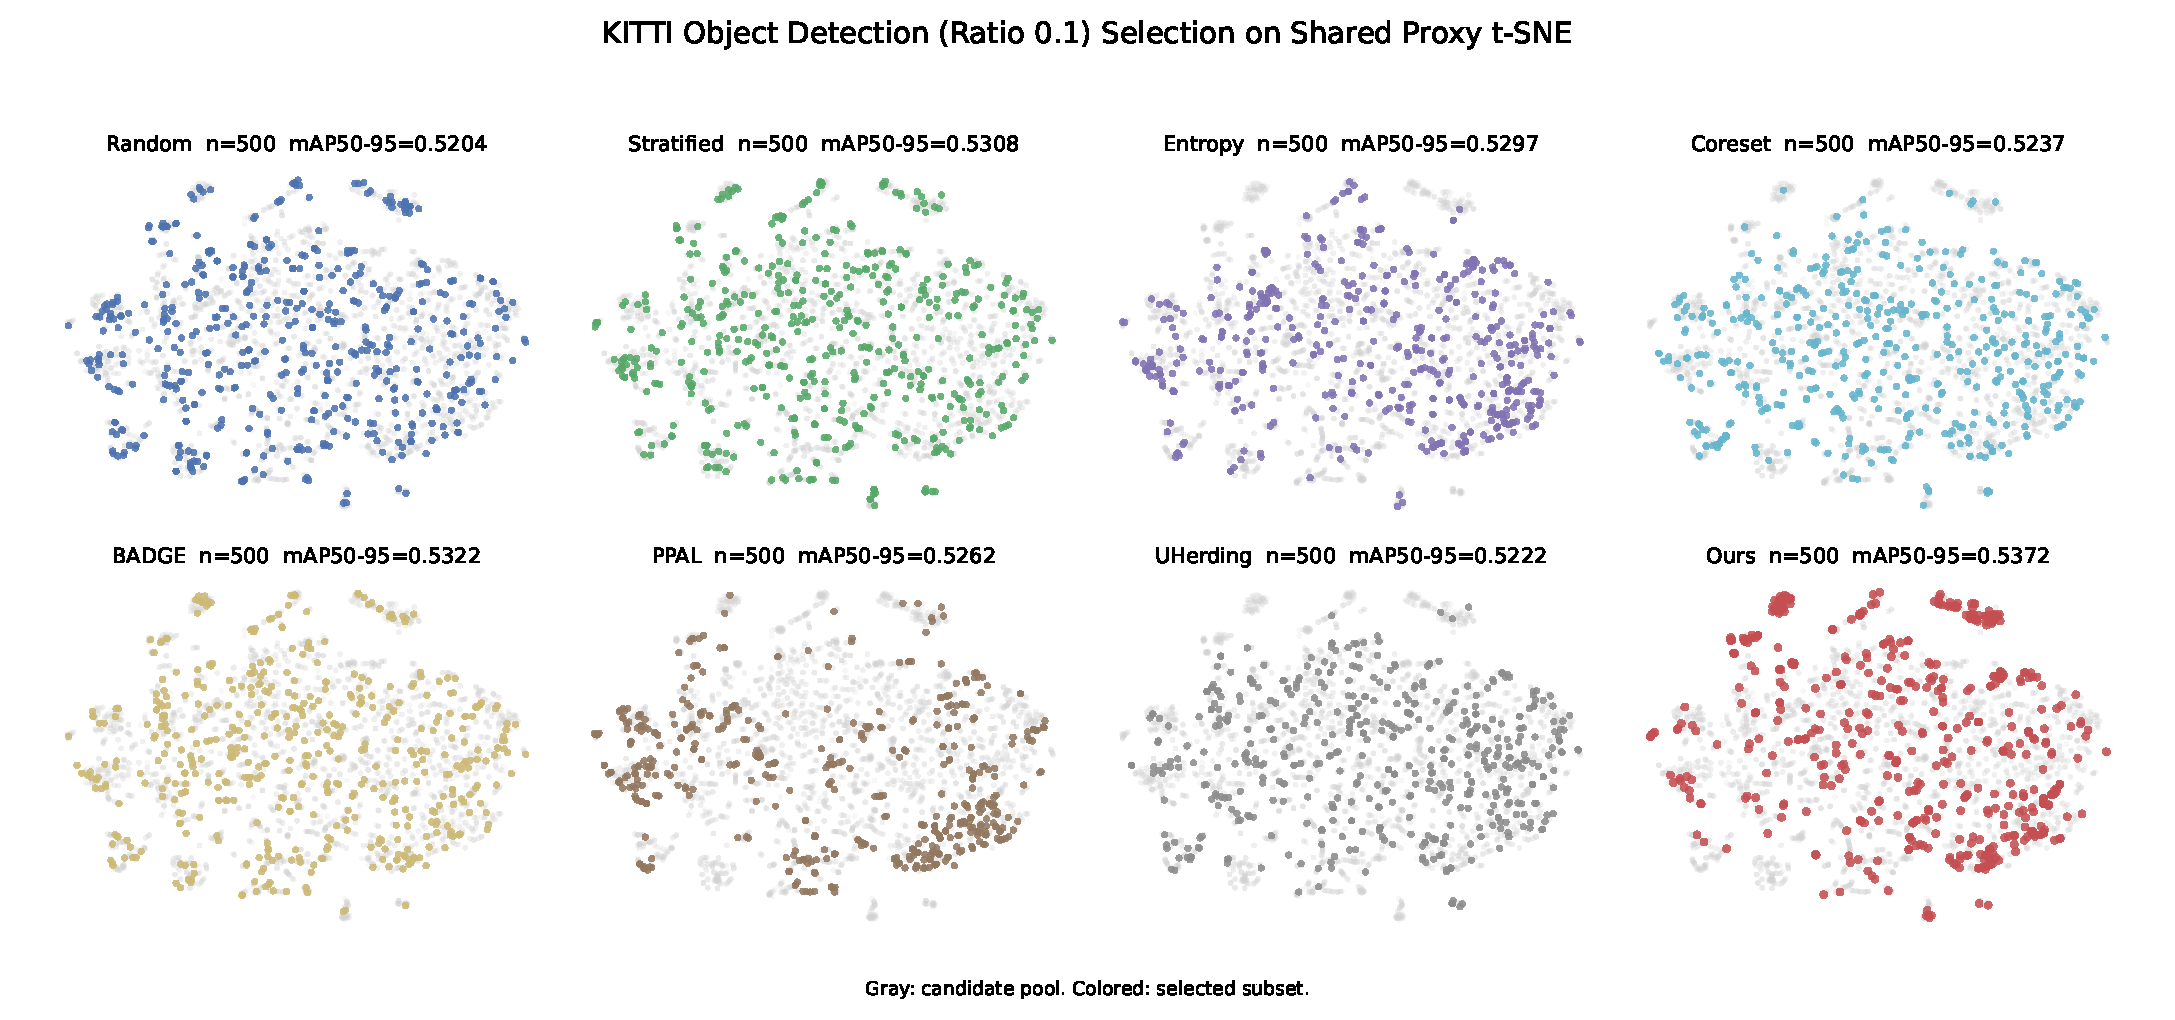
\includegraphics[width=\linewidth]{figures/ratio0p1_selection_tsne/kitti_red_cloudy_ratio0p1_selection_tsne.pdf}
\caption{KITTI object-detection ratio-$0.10$ selected subsets visualized on a shared source-image t-SNE embedding ($n=500$).}
\label{fig:tsne-r01-kitti}
\end{figure*}

% \begin{figure}[p]
% \centering
% 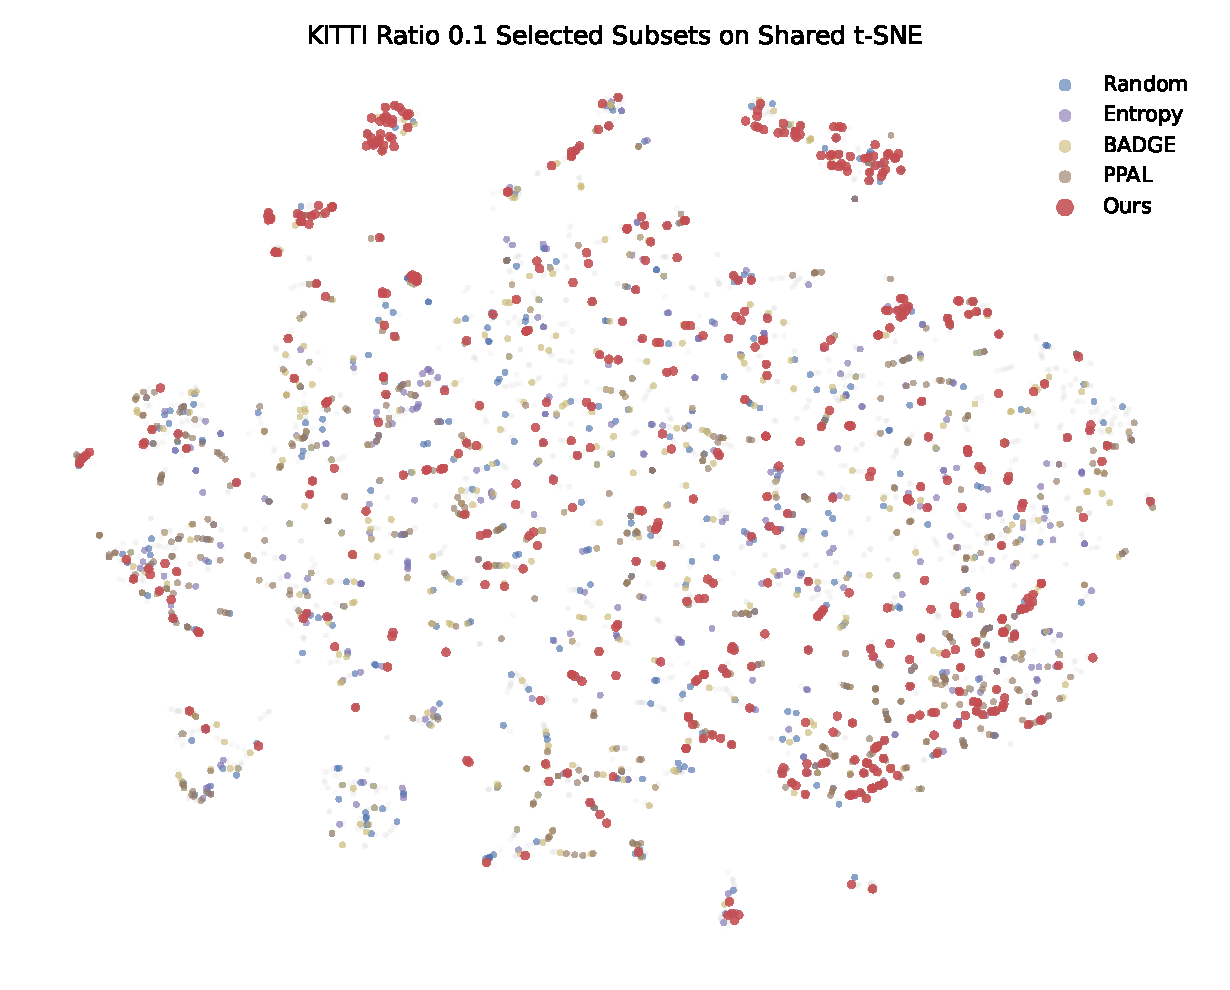
\includegraphics[width=0.86\linewidth]{figures/ratio0p1_selection_tsne/kitti_red_cloudy_ratio0p1_selection_tsne_overlay.pdf}
% \caption{KITTI object-detection ratio-$0.10$ overlay view for selected active-learning baselines and \model.}
% \label{fig:tsne-overlay-r01-kitti}
% \end{figure}

% \begin{figure}[p]
% \centering
% \includegraphics[width=\linewidth]{figures/ratio0p05_selection_tsne/imagenet_controlnet_ratio0p05_selection_tsne.pdf}
% \caption{ImageNet ratio-$0.05$ selected subsets visualized on a shared source-image t-SNE embedding.}
% \label{fig:tsne-r005-imagenet}
% \end{figure}

\begin{figure*}[p]
\centering
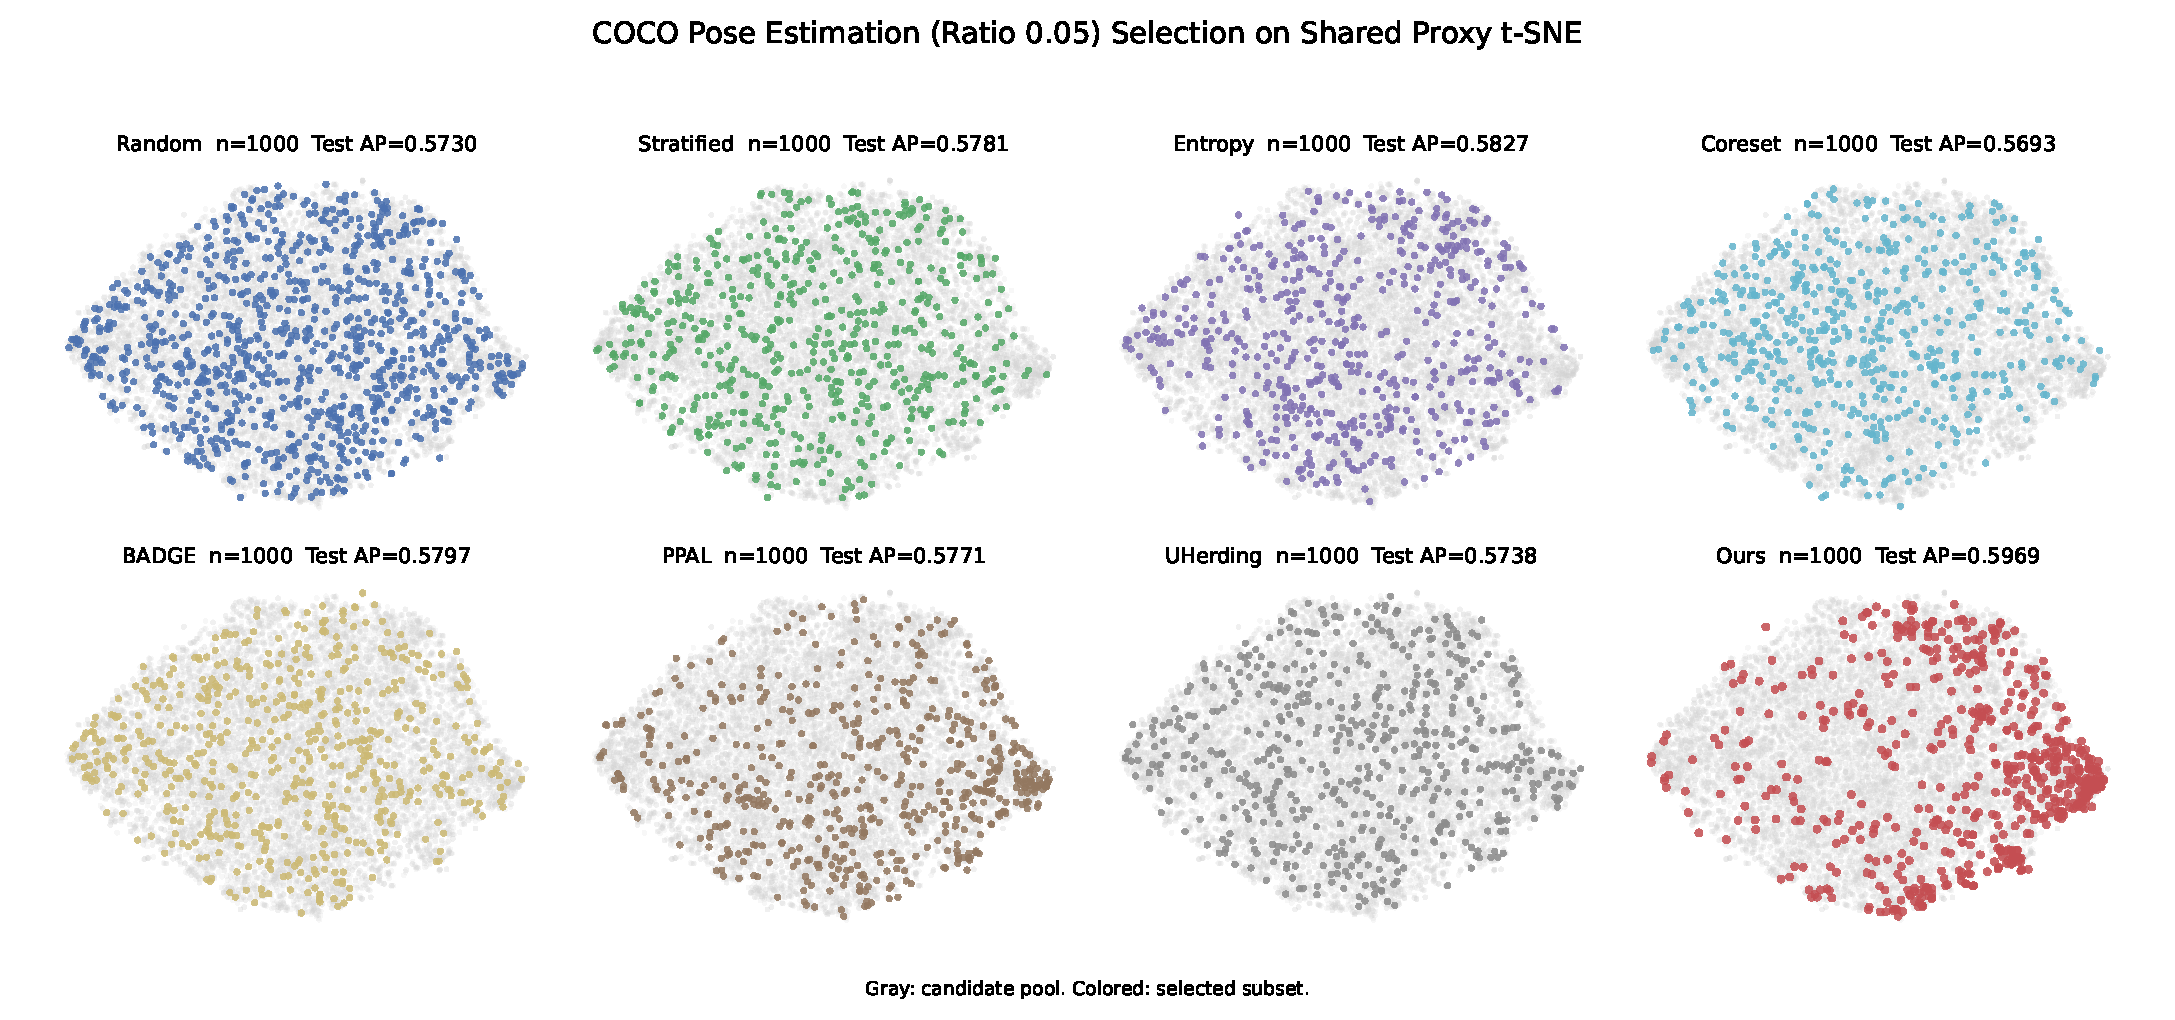
\includegraphics[width=\linewidth]{figures/ratio0p05_selection_tsne/coco_brown_rainy_ratio0p05_selection_tsne.pdf}
\caption{COCO pose-estimation ratio-$0.05$ selected subsets visualized on a shared source-image t-SNE embedding ($n=1{,}000$). Each method selects an identical source budget of $1{,}000$ training images from the $N=20{,}000$ candidate pool. Subpanel titles report downstream test AP values matching the constrained-budget evaluations in Table~\ref{tab:constrained-source-budget}.}
\label{fig:tsne-r005-coco}
\end{figure*}

\begin{figure*}[p]
\centering
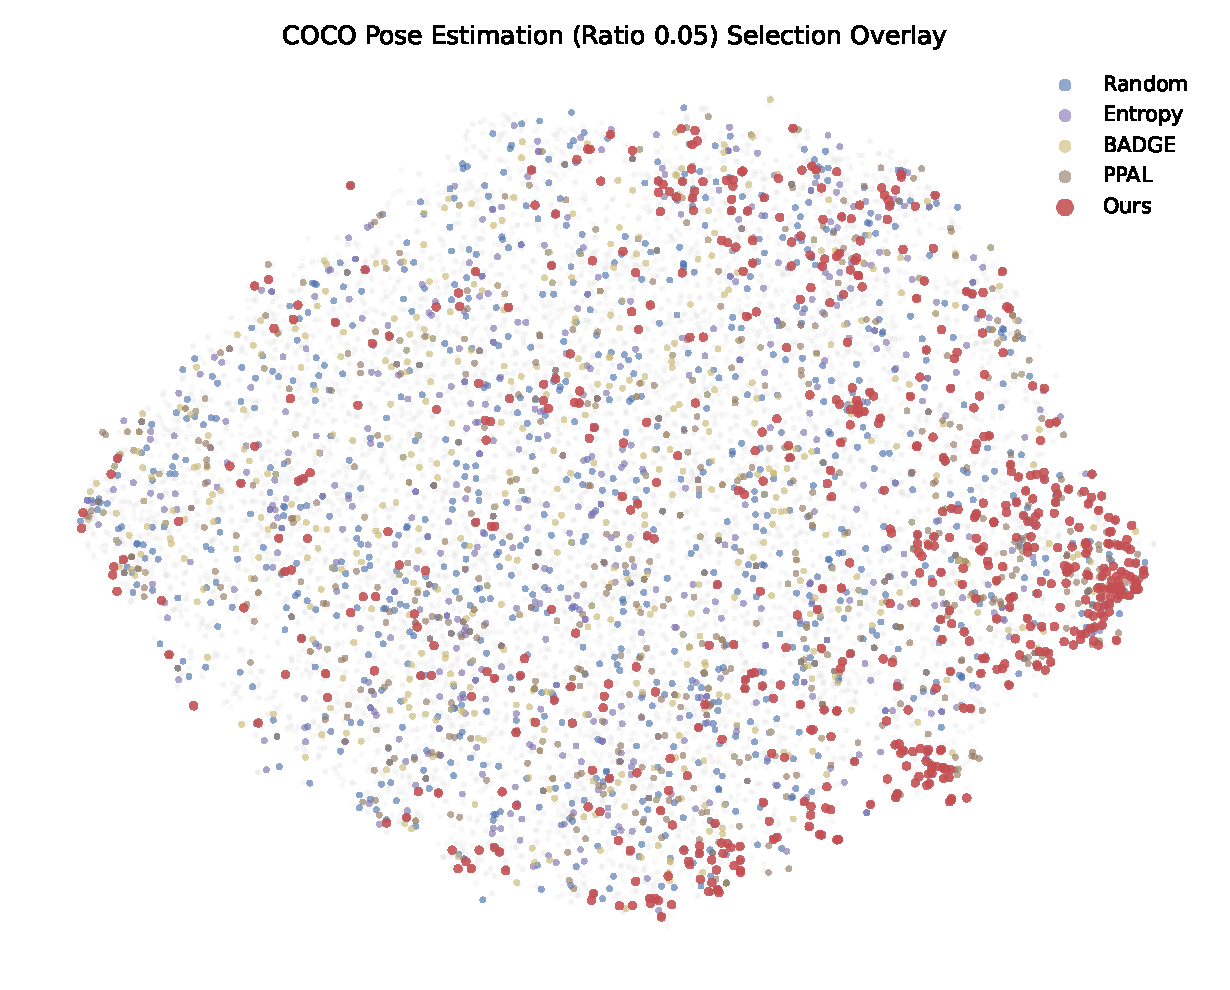
\includegraphics[width=0.86\linewidth]{figures/ratio0p05_selection_tsne/coco_brown_rainy_ratio0p05_selection_tsne_overlay.pdf}
\caption{COCO pose-estimation ratio-$0.05$ overlay view for selected active-learning baselines and \model ($n=1{,}000$).}
\label{fig:tsne-overlay-r005-coco}
\end{figure*}

%% \section{Selection Overlap as an Attribute-Information Diagnostic}
% \label{app:overlap-diagnostic}

% This section formalizes what the selection-overlap plots test. Standard active learning selectors rank or cover examples using information such as logits, losses, uncertainty scores, feature embeddings, gradient embeddings, image distances, and sometimes class labels. Let $H_i$ denote all such non-attribute information for source example $x_i$. Our selector additionally observes structured attribute metadata
% \begin{equation}
% A_i=\big(a(x_i):a\in\attrs\big).
% \end{equation}
% The comparison is not only between two scoring formulas. The selectors use different information fields: generic AL is attribute-agnostic when it is a function of $H_i$, while the proposed selector is a function of both $H_i$ and $A_i$ through rarity, generated-data frequency, and class-aware re-ranking.

% The overlap plots therefore answer a specific question: is \model merely reproducing the same subset chosen by uncertainty, CoreSet, BADGE, PPAL, Uncertainty Herding, or random selection? Low overlap by itself is not a performance guarantee. However, when low overlap is paired with the slice-enrichment result in Proposition~\ref{prop:rarity-margin} and with improved downstream repair, it supports a stronger interpretation: the gain comes from a semantic selection direction that is not already captured by generic AL signals.

% \begin{tcolorbox}[
%     colback=blue!2!white,
%     colframe=blue!20!white,
%     arc=3pt,
%     boxrule=1pt,
%     drop shadow,
%     breakable
% ]
% \begin{proposition}[Random-overlap scale for attribute-agnostic selectors]
% \label{prop:random-overlap-scale}
% Let the source pool be partitioned into groups $\mathcal{G}_1,\ldots,\mathcal{G}_K$, such as classes or class-allocation bins, with $N_g=|\mathcal{G}_g|$. Let $S_A$ be an attribute-driven selected set and let $S_H$ be an attribute-agnostic selected set. Suppose $S_A$ selects $m_{A,g}$ examples from group $g$ and $S_H$ selects $m_{H,g}$ examples from group $g$. If, conditional on the group counts and on $S_A$, the attribute-agnostic selector is exchangeable with respect to membership in $S_A$ inside each group, then
% \begin{equation}
% \mathbb{E}\big[|S_A\cap S_H|\mid S_A\big]
% =
% \sum_{g=1}^K \frac{m_{A,g}m_{H,g}}{N_g}.
% \end{equation}
% In the ungrouped case, if both selectors choose $m=rN$ examples from a pool of size $N$, then
% \begin{equation}
% \mathbb{E}\big[|S_A\cap S_H|\mid S_A\big]=r^2N.
% \end{equation}
% Moreover, as $N\rightarrow\infty$ with fixed ratio $r$, the Jaccard overlap
% \begin{equation}
% J(S_A,S_H)=\frac{|S_A\cap S_H|}{|S_A\cup S_H|}
% \end{equation}
% converges in probability to the random-subset scale
% \begin{equation}
% J_{\mathrm{rand}}(r)=\frac{r}{2-r}.
% \end{equation}
% \end{proposition}
% \end{tcolorbox}

% \begin{tcolorbox}[
%     colback=green!2!white,
%     colframe=green!20!white,
%     arc=3pt,
%     boxrule=1pt,
%     drop shadow,
%     breakable
% ]
% \begin{proof}
% Fix a group $\mathcal{G}_g$ and condition on $S_A$. Since $S_H$ is exchangeable with respect to membership in $S_A$ within the group, selecting $m_{H,g}$ examples from $\mathcal{G}_g$ gives a hypergeometric intersection with mean
% \begin{equation}
% m_{H,g}\frac{m_{A,g}}{N_g}.
% \end{equation}
% Summing over groups gives the first claim. In the ungrouped case this reduces to $m^2/N=r^2N$. Hypergeometric concentration gives $|S_A\cap S_H|/N\rightarrow r^2$ in probability. Since $|S_A\cup S_H|=2rN-|S_A\cap S_H|$, the continuous mapping theorem gives
% \begin{equation}
% \frac{|S_A\cap S_H|}{|S_A\cup S_H|}
% \rightarrow
% \frac{r^2}{2r-r^2}
% =
% \frac{r}{2-r}.
% \end{equation}
% \end{proof}
% \end{tcolorbox}

% Proposition~\ref{prop:random-overlap-scale} gives a useful diagnostic. If an attribute-aware selector and an attribute-agnostic AL selector have Jaccard overlap close to $J_{\mathrm{rand}}(r)$, then the two selected sets are no more similar than two independent budget-matched subsets at that ratio. This is exactly what one expects when the attributes carry selection information not present in the AL variables $H_i$. Conversely, if a conventional AL method were already aligned with the discovered attribute slice, its overlap with the selected set from \model would tend to rise above this random-overlap scale.

% The ungrouped value $J_{\mathrm{rand}}(r)$ is a useful lower reference for selectors that share a group allocation over imbalanced groups. Suppose two exchangeable selectors both choose $B_g$ examples from group $g$, with $\sum_g B_g=rN$ and $\sum_g N_g=N$. Proposition~\ref{prop:random-overlap-scale} gives expected intersection $\sum_g B_g^2/N_g$, and Cauchy--Schwarz gives
% \begin{equation}
% \sum_g \frac{B_g^2}{N_g}
% \geq
% \frac{\left(\sum_g B_g\right)^2}{\sum_g N_g}
% =
% r^2N,
% \end{equation}
% with equality only when $B_g/N_g$ is constant across groups. For fixed total budget, the large-pool Jaccard reference is an increasing function of the intersection size, so class-aware allocations on imbalanced datasets can have a random-overlap scale slightly above the ungrouped limit. This helps explain why the baseline--baseline averages in Table~\ref{tab:selection-overlap-summary} are consistently above $J_{\mathrm{rand}}(r)$ when the baselines share similar class-allocation effects. When two methods use different group allocations, the full grouped expression in Proposition~\ref{prop:random-overlap-scale} is the appropriate reference.

% \begin{tcolorbox}[
%     colback=blue!2!white,
%     colframe=blue!20!white,
%     arc=3pt,
%     boxrule=1pt,
%     drop shadow,
%     breakable
% ]
% \begin{proposition}[Non-redundant repair utility]
% \label{prop:nonredundant-utility}
% Assume the repair-utility model from Appendix~\ref{app:theory-analysis},
% \begin{equation}
% U(S)=u_0|S|+(u_T-u_0)|S\cap T|,\qquad u_T>u_0,
% \end{equation}
% where $T$ is the target failure slice. Suppose \model satisfies the deterministic rare-slice enrichment condition in Proposition~\ref{prop:deterministic-enrichment}, while an attribute-agnostic selector satisfies the conditional-independence condition in Proposition~\ref{prop:al-target-alignment}, under the same per-class allocations $B_c$. Then the expected utility advantage of \model over the attribute-agnostic selector is at least
% \begin{equation}
% (u_T-u_0)
% \sum_c
% \left[
% \min\{B_c,|T_c|\}
% -
% B_c\frac{|T_c|}{N_c}
% \right].
% \end{equation}
% This lower bound is strict whenever at least one class has $0<|T_c|<N_c$ and receives a positive budget that does not occupy the whole class, i.e., $0<B_c<N_c$. If, in addition, the empirical Jaccard overlap between the two selected sets is close to $J_{\mathrm{rand}}(r)$, then this utility advantage cannot be explained by selecting the same source examples as the attribute-agnostic baseline.
% \end{proposition}
% \end{tcolorbox}

% \begin{tcolorbox}[
%     colback=green!2!white,
%     colframe=green!20!white,
%     arc=3pt,
%     boxrule=1pt,
%     drop shadow,
%     breakable
% ]
% \begin{proof}
% Proposition~\ref{prop:deterministic-enrichment} gives at least $\min\{B_c,|T_c|\}$ target examples for \model in class $c$. Proposition~\ref{prop:al-target-alignment} gives $B_c|T_c|/N_c$ target examples in expectation for an attribute-agnostic selector under the same class allocation. Since both selectors use the same total budget, the $u_0|S|$ term cancels. Multiplying the difference in target-slice support by the marginal utility gap $u_T-u_0$ gives the stated bound. The strictness condition follows because $\min\{B_c,|T_c|\}>B_c|T_c|/N_c$ whenever a nontrivial target slice receives budget without occupying the whole class. The final statement follows from Proposition~\ref{prop:random-overlap-scale}: near-random Jaccard overlap means the two selectors are not choosing substantially the same subset beyond what the sampling ratio itself forces.
% \end{proof}
% \end{tcolorbox}

% Table~\ref{tab:selection-overlap-summary} summarizes the observed Jaccard overlaps between selected subsets. The t-SNE coordinates are not used in the calculation; the metric is computed only from selected-set membership. Across ratios, the average overlap between \model and the baselines is close to the random-subset scale $J_{\mathrm{rand}}(r)$ and lower than the average pairwise overlap among baselines. This supports the interpretation that \model operates along a different semantic information direction rather than imitating a conventional AL heuristic.

% \begin{table}[htbp]
% \centering
% \caption{Selection-overlap diagnostic. ``Ours--baseline'' is the mean Jaccard overlap between \model and the non-attribute baselines. ``Baseline--baseline'' is the mean pairwise Jaccard overlap among non-attribute baselines. Each row averages over ImageNet, CelebA, COCO, and KITTI.}
% \label{tab:selection-overlap-summary}
% \begin{tabular}{c c c c c}
% \toprule
% \rowcolor{sectiongray} \textbf{Selection ratio} & $\boldsymbol{J_{\mathrm{rand}}(r)}$ & \textbf{Datasets} & \textbf{Ours--baseline} & \textbf{Baseline--baseline} \\
% \midrule
% $0.10$ & $0.0526$ & $4$ & $0.0533$ & $0.0554$ \\
% $0.30$ & $0.1765$ & $4$ & $0.1766$ & $0.1828$ \\
% $0.50$ & $0.3333$ & $4$ & $0.3323$ & $0.3416$ \\
% \bottomrule
% \end{tabular}
% \end{table}

% The corresponding heatmaps are shown in Figures~\ref{fig:selection-overlap-r01}, \ref{fig:selection-overlap-r03}, and~\ref{fig:selection-overlap-r05}. The diagonal entries are one by definition; off-diagonal entries measure pairwise Jaccard overlap between selected source subsets.

% \begin{figure}[p]
% \centering
% \begin{subfigure}{0.48\linewidth}
% \centering
% \includegraphics[width=\linewidth]{figures/ratio0p1_selection_overlap/imagenet_controlnet_ratio0p1_selection_overlap_jaccard.png}
% \caption{ImageNet}
% \end{subfigure}
% \hfill
% \begin{subfigure}{0.48\linewidth}
% \centering
% \includegraphics[width=\linewidth]{figures/ratio0p1_selection_overlap/celeba_redhair_brownskin_sademotion_ratio0p1_selection_overlap_jaccard.png}
% \caption{CelebA}
% \end{subfigure}

% \vspace{0.6em}
% \begin{subfigure}{0.48\linewidth}
% \centering
% \includegraphics[width=\linewidth]{figures/ratio0p1_selection_overlap/coco_brown_rainy_ratio0p1_selection_overlap_jaccard.png}
% \caption{COCO}
% \end{subfigure}
% \hfill
% \begin{subfigure}{0.48\linewidth}
% \centering
% \includegraphics[width=\linewidth]{figures/ratio0p1_selection_overlap/kitti_red_cloudy_ratio0p1_selection_overlap_jaccard.png}
% \caption{KITTI}
% \end{subfigure}
% \caption{Pairwise Jaccard overlap among ratio $0.10$ selected subsets.}
% \label{fig:selection-overlap-r01}
% \end{figure}

% \begin{figure}[p]
% \centering
% \begin{subfigure}{0.48\linewidth}
% \centering
% \includegraphics[width=\linewidth]{figures/ratio0p3_selection_overlap/imagenet_controlnet_ratio0p3_selection_overlap_jaccard.png}
% \caption{ImageNet}
% \end{subfigure}
% \hfill
% \begin{subfigure}{0.48\linewidth}
% \centering
% \includegraphics[width=\linewidth]{figures/ratio0p3_selection_overlap/celeba_redhair_brownskin_sademotion_ratio0p3_selection_overlap_jaccard.png}
% \caption{CelebA}
% \end{subfigure}

% \vspace{0.6em}
% \begin{subfigure}{0.48\linewidth}
% \centering
% \includegraphics[width=\linewidth]{figures/ratio0p3_selection_overlap/coco_brown_rainy_ratio0p3_selection_overlap_jaccard.png}
% \caption{COCO}
% \end{subfigure}
% \hfill
% \begin{subfigure}{0.48\linewidth}
% \centering
% \includegraphics[width=\linewidth]{figures/ratio0p3_selection_overlap/kitti_red_cloudy_ratio0p3_selection_overlap_jaccard.png}
% \caption{KITTI}
% \end{subfigure}
% \caption{Pairwise Jaccard overlap among ratio $0.30$ selected subsets.}
% \label{fig:selection-overlap-r03}
% \end{figure}

% \begin{figure}[p]
% \centering
% \begin{subfigure}{0.48\linewidth}
% \centering
% \includegraphics[width=\linewidth]{figures/ratio0p5_selection_overlap/imagenet_controlnet_ratio0p5_selection_overlap_jaccard.png}
% \caption{ImageNet}
% \end{subfigure}
% \hfill
% \begin{subfigure}{0.48\linewidth}
% \centering
% \includegraphics[width=\linewidth]{figures/ratio0p5_selection_overlap/celeba_redhair_brownskin_sademotion_ratio0p5_selection_overlap_jaccard.png}
% \caption{CelebA}
% \end{subfigure}

% \vspace{0.6em}
% \begin{subfigure}{0.48\linewidth}
% \centering
% \includegraphics[width=\linewidth]{figures/ratio0p5_selection_overlap/coco_brown_rainy_ratio0p5_selection_overlap_jaccard.png}
% \caption{COCO}
% \end{subfigure}
% \hfill
% \begin{subfigure}{0.48\linewidth}
% \centering
% \includegraphics[width=\linewidth]{figures/ratio0p5_selection_overlap/kitti_red_cloudy_ratio0p5_selection_overlap_jaccard.png}
% \caption{KITTI}
% \end{subfigure}
% \caption{Pairwise Jaccard overlap among ratio $0.50$ selected subsets.}
% \label{fig:selection-overlap-r05}
% \end{figure}

% These numbers and figures should be read together with the propositions above. Lower overlap alone does not prove that a subset improves the model. The results instead establish that \model is not redundant with uncertainty, diversity, geometry, detector-difficulty, or gradient-embedding selectors. This behavior matches the theory: the selector spends budget on an attribute-defined repair signal that the generic AL variables do not explicitly encode.

\section{Limitations and Practical Considerations}
\label{app:limitations}

\textbf{VLM dependency.}\\
\model assumes that source images have VLM-assigned attribute records before selection and relies on accurate VLM annotation.

\vspace{0.5em}
\textbf{Attribute vocabulary coverage.}\\
\model can only target failure modes described by the available attribute vocabulary. If an important failure factor is missing from $\attrs$ or merged into a coarse closed-set value, the selector cannot explicitly prioritize it.

\vspace{0.5em}
\textbf{Marginal versus conjunction rarity.}\\
The current score sums per-field marginal counts. A diagnosed conjunction can therefore be rare even when each of its marginal attribute values is common. In that case, the pairwise marginal-rarity condition in Appendix~\ref{app:theory-analysis} may fail, and the current theory does not guarantee enrichment of the conjunction. A joint-count score could target such intersections directly, but it would define a different selector that requires separate experiments.

\vspace{0.5em}
\textbf{Generated-data quality.}\\
\model chooses source examples that complement generated repair images, but it does not correct failures in the generator itself. If generated images miss the target attributes, change labels, or introduce artifacts, the absolute repair gains can decrease even when source selection remains useful.

\clearpage

\end{document}
